% Options for packages loaded elsewhere
\PassOptionsToPackage{unicode}{hyperref}
\PassOptionsToPackage{hyphens}{url}
%
\documentclass[
]{article}
\usepackage{amsmath,amssymb}
\usepackage{lmodern}
\usepackage{iftex}
\ifPDFTeX
  \usepackage[T1]{fontenc}
  \usepackage[utf8]{inputenc}
  \usepackage{textcomp} % provide euro and other symbols
\else % if luatex or xetex
  \usepackage{unicode-math}
  \defaultfontfeatures{Scale=MatchLowercase}
  \defaultfontfeatures[\rmfamily]{Ligatures=TeX,Scale=1}
\fi
% Use upquote if available, for straight quotes in verbatim environments
\IfFileExists{upquote.sty}{\usepackage{upquote}}{}
\IfFileExists{microtype.sty}{% use microtype if available
  \usepackage[]{microtype}
  \UseMicrotypeSet[protrusion]{basicmath} % disable protrusion for tt fonts
}{}
\makeatletter
\@ifundefined{KOMAClassName}{% if non-KOMA class
  \IfFileExists{parskip.sty}{%
    \usepackage{parskip}
  }{% else
    \setlength{\parindent}{0pt}
    \setlength{\parskip}{6pt plus 2pt minus 1pt}}
}{% if KOMA class
  \KOMAoptions{parskip=half}}
\makeatother
\usepackage{xcolor}
\usepackage[margin=1in]{geometry}
\usepackage{color}
\usepackage{fancyvrb}
\newcommand{\VerbBar}{|}
\newcommand{\VERB}{\Verb[commandchars=\\\{\}]}
\DefineVerbatimEnvironment{Highlighting}{Verbatim}{commandchars=\\\{\}}
% Add ',fontsize=\small' for more characters per line
\usepackage{framed}
\definecolor{shadecolor}{RGB}{248,248,248}
\newenvironment{Shaded}{\begin{snugshade}}{\end{snugshade}}
\newcommand{\AlertTok}[1]{\textcolor[rgb]{0.94,0.16,0.16}{#1}}
\newcommand{\AnnotationTok}[1]{\textcolor[rgb]{0.56,0.35,0.01}{\textbf{\textit{#1}}}}
\newcommand{\AttributeTok}[1]{\textcolor[rgb]{0.77,0.63,0.00}{#1}}
\newcommand{\BaseNTok}[1]{\textcolor[rgb]{0.00,0.00,0.81}{#1}}
\newcommand{\BuiltInTok}[1]{#1}
\newcommand{\CharTok}[1]{\textcolor[rgb]{0.31,0.60,0.02}{#1}}
\newcommand{\CommentTok}[1]{\textcolor[rgb]{0.56,0.35,0.01}{\textit{#1}}}
\newcommand{\CommentVarTok}[1]{\textcolor[rgb]{0.56,0.35,0.01}{\textbf{\textit{#1}}}}
\newcommand{\ConstantTok}[1]{\textcolor[rgb]{0.00,0.00,0.00}{#1}}
\newcommand{\ControlFlowTok}[1]{\textcolor[rgb]{0.13,0.29,0.53}{\textbf{#1}}}
\newcommand{\DataTypeTok}[1]{\textcolor[rgb]{0.13,0.29,0.53}{#1}}
\newcommand{\DecValTok}[1]{\textcolor[rgb]{0.00,0.00,0.81}{#1}}
\newcommand{\DocumentationTok}[1]{\textcolor[rgb]{0.56,0.35,0.01}{\textbf{\textit{#1}}}}
\newcommand{\ErrorTok}[1]{\textcolor[rgb]{0.64,0.00,0.00}{\textbf{#1}}}
\newcommand{\ExtensionTok}[1]{#1}
\newcommand{\FloatTok}[1]{\textcolor[rgb]{0.00,0.00,0.81}{#1}}
\newcommand{\FunctionTok}[1]{\textcolor[rgb]{0.00,0.00,0.00}{#1}}
\newcommand{\ImportTok}[1]{#1}
\newcommand{\InformationTok}[1]{\textcolor[rgb]{0.56,0.35,0.01}{\textbf{\textit{#1}}}}
\newcommand{\KeywordTok}[1]{\textcolor[rgb]{0.13,0.29,0.53}{\textbf{#1}}}
\newcommand{\NormalTok}[1]{#1}
\newcommand{\OperatorTok}[1]{\textcolor[rgb]{0.81,0.36,0.00}{\textbf{#1}}}
\newcommand{\OtherTok}[1]{\textcolor[rgb]{0.56,0.35,0.01}{#1}}
\newcommand{\PreprocessorTok}[1]{\textcolor[rgb]{0.56,0.35,0.01}{\textit{#1}}}
\newcommand{\RegionMarkerTok}[1]{#1}
\newcommand{\SpecialCharTok}[1]{\textcolor[rgb]{0.00,0.00,0.00}{#1}}
\newcommand{\SpecialStringTok}[1]{\textcolor[rgb]{0.31,0.60,0.02}{#1}}
\newcommand{\StringTok}[1]{\textcolor[rgb]{0.31,0.60,0.02}{#1}}
\newcommand{\VariableTok}[1]{\textcolor[rgb]{0.00,0.00,0.00}{#1}}
\newcommand{\VerbatimStringTok}[1]{\textcolor[rgb]{0.31,0.60,0.02}{#1}}
\newcommand{\WarningTok}[1]{\textcolor[rgb]{0.56,0.35,0.01}{\textbf{\textit{#1}}}}
\usepackage{longtable,booktabs,array}
\usepackage{calc} % for calculating minipage widths
% Correct order of tables after \paragraph or \subparagraph
\usepackage{etoolbox}
\makeatletter
\patchcmd\longtable{\par}{\if@noskipsec\mbox{}\fi\par}{}{}
\makeatother
% Allow footnotes in longtable head/foot
\IfFileExists{footnotehyper.sty}{\usepackage{footnotehyper}}{\usepackage{footnote}}
\makesavenoteenv{longtable}
\usepackage{graphicx}
\makeatletter
\def\maxwidth{\ifdim\Gin@nat@width>\linewidth\linewidth\else\Gin@nat@width\fi}
\def\maxheight{\ifdim\Gin@nat@height>\textheight\textheight\else\Gin@nat@height\fi}
\makeatother
% Scale images if necessary, so that they will not overflow the page
% margins by default, and it is still possible to overwrite the defaults
% using explicit options in \includegraphics[width, height, ...]{}
\setkeys{Gin}{width=\maxwidth,height=\maxheight,keepaspectratio}
% Set default figure placement to htbp
\makeatletter
\def\fps@figure{htbp}
\makeatother
\setlength{\emergencystretch}{3em} % prevent overfull lines
\providecommand{\tightlist}{%
  \setlength{\itemsep}{0pt}\setlength{\parskip}{0pt}}
\setcounter{secnumdepth}{5}
\ifLuaTeX
  \usepackage{selnolig}  % disable illegal ligatures
\fi
\IfFileExists{bookmark.sty}{\usepackage{bookmark}}{\usepackage{hyperref}}
\IfFileExists{xurl.sty}{\usepackage{xurl}}{} % add URL line breaks if available
\urlstyle{same} % disable monospaced font for URLs
\hypersetup{
  pdftitle={Risk-Evaluation: Breast Cancer Royston-Altman},
  pdfauthor={Jose Tamez},
  hidelinks,
  pdfcreator={LaTeX via pandoc}}

\title{Risk-Evaluation: Breast Cancer Royston-Altman}
\author{Jose Tamez}
\date{2023-05-18}

\begin{document}
\maketitle

{
\setcounter{tocdepth}{2}
\tableofcontents
}
\hypertarget{evaluation-of-risk-survival-models}{%
\section{Evaluation of RISK survival
models}\label{evaluation-of-risk-survival-models}}

This document highlights the use of

\begin{itemize}
\item
  RRPlot(),
\item
  CoxRiskCalibration(), and
\item
  CalibrationProbPoissonRisk(),
\end{itemize}

for the evaluation (RRPlot), and calibration of cox models
(CoxRiskCalibration) or logistic models (CalibrationProbPoissonRisk) of
survival data.

Furthermore, it can be used to evaluate any Risk index that reruns the
probability of a future event on external data-set.

This document will use the survival::rotterdam, and survival::gbsg
data-sets to train and predict the risk of cancer recurrence after
surgery. Both Cox and Logistic models will be trained and evaluated.

Here are some sample plots returned by the evaluated functions:

\hypertarget{the-libraries}{%
\subsection{The libraries}\label{the-libraries}}

\begin{Shaded}
\begin{Highlighting}[]
\FunctionTok{library}\NormalTok{(survival)}
\FunctionTok{library}\NormalTok{(FRESA.CAD)}
\end{Highlighting}
\end{Shaded}

\begin{verbatim}
## Loading required package: Rcpp
\end{verbatim}

\begin{verbatim}
## Loading required package: stringr
\end{verbatim}

\begin{verbatim}
## Loading required package: miscTools
\end{verbatim}

\begin{verbatim}
## Loading required package: Hmisc
\end{verbatim}

\begin{verbatim}
## 
## Attaching package: 'Hmisc'
\end{verbatim}

\begin{verbatim}
## The following objects are masked from 'package:base':
## 
##     format.pval, units
\end{verbatim}

\begin{verbatim}
## Loading required package: pROC
\end{verbatim}

\begin{verbatim}
## Type 'citation("pROC")' for a citation.
\end{verbatim}

\begin{verbatim}
## 
## Attaching package: 'pROC'
\end{verbatim}

\begin{verbatim}
## The following objects are masked from 'package:stats':
## 
##     cov, smooth, var
\end{verbatim}

\begin{Shaded}
\begin{Highlighting}[]
\NormalTok{op }\OtherTok{\textless{}{-}} \FunctionTok{par}\NormalTok{(}\AttributeTok{no.readonly =} \ConstantTok{TRUE}\NormalTok{)}
\NormalTok{pander}\SpecialCharTok{::}\FunctionTok{panderOptions}\NormalTok{(}\StringTok{\textquotesingle{}digits\textquotesingle{}}\NormalTok{, }\DecValTok{3}\NormalTok{)}
\NormalTok{pander}\SpecialCharTok{::}\FunctionTok{panderOptions}\NormalTok{(}\StringTok{\textquotesingle{}table.split.table\textquotesingle{}}\NormalTok{, }\DecValTok{400}\NormalTok{)}
\NormalTok{pander}\SpecialCharTok{::}\FunctionTok{panderOptions}\NormalTok{(}\StringTok{\textquotesingle{}keep.trailing.zeros\textquotesingle{}}\NormalTok{,}\ConstantTok{TRUE}\NormalTok{)}
\end{Highlighting}
\end{Shaded}

\hypertarget{breast-cancer-royston-altman-data}{%
\subsection{Breast Cancer Royston-Altman
data}\label{breast-cancer-royston-altman-data}}

\hypertarget{datagbsg-packagesurvival-and-datarotterdam-packagesurvival}{%
\subsubsection{data(gbsg, package=``survival'') and data(rotterdam,
package=``survival'')}\label{datagbsg-packagesurvival-and-datarotterdam-packagesurvival}}

\begin{Shaded}
\begin{Highlighting}[]
\NormalTok{gbsgdata }\OtherTok{\textless{}{-}}\NormalTok{ gbsg}
\FunctionTok{rownames}\NormalTok{(gbsgdata) }\OtherTok{\textless{}{-}}\NormalTok{ gbsgdata}\SpecialCharTok{$}\NormalTok{pid}
\NormalTok{gbsgdata}\SpecialCharTok{$}\NormalTok{pid }\OtherTok{\textless{}{-}} \ConstantTok{NULL}

\NormalTok{odata }\OtherTok{\textless{}{-}}\NormalTok{rotterdam}
\FunctionTok{rownames}\NormalTok{(odata) }\OtherTok{\textless{}{-}}\NormalTok{ odata}\SpecialCharTok{$}\NormalTok{pid}
\NormalTok{odata}\SpecialCharTok{$}\NormalTok{pid }\OtherTok{\textless{}{-}} \ConstantTok{NULL}
\NormalTok{odata}\SpecialCharTok{$}\NormalTok{rfstime }\OtherTok{\textless{}{-}}\NormalTok{ odata}\SpecialCharTok{$}\NormalTok{rtime}
\NormalTok{odata}\SpecialCharTok{$}\NormalTok{status }\OtherTok{\textless{}{-}}\NormalTok{ odata}\SpecialCharTok{$}\NormalTok{recur}
\NormalTok{odata}\SpecialCharTok{$}\NormalTok{rtime }\OtherTok{\textless{}{-}} \ConstantTok{NULL}
\NormalTok{odata}\SpecialCharTok{$}\NormalTok{recur }\OtherTok{\textless{}{-}} \ConstantTok{NULL}

\NormalTok{odata }\OtherTok{\textless{}{-}}\NormalTok{ odata[,}\FunctionTok{colnames}\NormalTok{(odata) }\SpecialCharTok{\%in\%} \FunctionTok{colnames}\NormalTok{(gbsgdata)]}

\NormalTok{odata}\SpecialCharTok{$}\NormalTok{size }\OtherTok{\textless{}{-}} \DecValTok{10}\SpecialCharTok{*}\NormalTok{(odata}\SpecialCharTok{$}\NormalTok{size}\SpecialCharTok{==}\StringTok{"\textless{}=20"}\NormalTok{) }\SpecialCharTok{+} 
  \DecValTok{35}\SpecialCharTok{*}\NormalTok{(odata}\SpecialCharTok{$}\NormalTok{size}\SpecialCharTok{==}\StringTok{"20{-}50"}\NormalTok{) }\SpecialCharTok{+} 
  \DecValTok{60}\SpecialCharTok{*}\NormalTok{(odata}\SpecialCharTok{$}\NormalTok{size}\SpecialCharTok{==}\StringTok{"\textgreater{}50"}\NormalTok{)}

\NormalTok{data }\OtherTok{\textless{}{-}} \FunctionTok{as.data.frame}\NormalTok{(}\FunctionTok{model.matrix}\NormalTok{(}\FunctionTok{Surv}\NormalTok{(rfstime,status)}\SpecialCharTok{\textasciitilde{}}\NormalTok{.}\SpecialCharTok{*}\NormalTok{.,odata))}

\NormalTok{data}\SpecialCharTok{$}\StringTok{\textasciigrave{}}\AttributeTok{(Intercept)}\StringTok{\textasciigrave{}} \OtherTok{\textless{}{-}} \ConstantTok{NULL}

\NormalTok{dataBrestCancerTrain }\OtherTok{\textless{}{-}} \FunctionTok{cbind}\NormalTok{(}\AttributeTok{time=}\NormalTok{odata[}\FunctionTok{rownames}\NormalTok{(data),}\StringTok{"rfstime"}\NormalTok{],}\AttributeTok{status=}\NormalTok{odata[}\FunctionTok{rownames}\NormalTok{(data),}\StringTok{"status"}\NormalTok{],data)}

\FunctionTok{colnames}\NormalTok{(dataBrestCancerTrain) }\OtherTok{\textless{}{-}}\FunctionTok{str\_replace\_all}\NormalTok{(}\FunctionTok{colnames}\NormalTok{(dataBrestCancerTrain),}\StringTok{":"}\NormalTok{,}\StringTok{"\_"}\NormalTok{)}
\FunctionTok{colnames}\NormalTok{(dataBrestCancerTrain) }\OtherTok{\textless{}{-}}\FunctionTok{str\_replace\_all}\NormalTok{(}\FunctionTok{colnames}\NormalTok{(dataBrestCancerTrain),}\StringTok{" "}\NormalTok{,}\StringTok{""}\NormalTok{)}
\FunctionTok{colnames}\NormalTok{(dataBrestCancerTrain) }\OtherTok{\textless{}{-}}\FunctionTok{str\_replace\_all}\NormalTok{(}\FunctionTok{colnames}\NormalTok{(dataBrestCancerTrain),}\StringTok{"}\SpecialCharTok{\textbackslash{}\textbackslash{}}\StringTok{."}\NormalTok{,}\StringTok{"\_"}\NormalTok{)}
\FunctionTok{colnames}\NormalTok{(dataBrestCancerTrain) }\OtherTok{\textless{}{-}}\FunctionTok{str\_replace\_all}\NormalTok{(}\FunctionTok{colnames}\NormalTok{(dataBrestCancerTrain),}\StringTok{"{-}"}\NormalTok{,}\StringTok{"\_"}\NormalTok{)}
\FunctionTok{colnames}\NormalTok{(dataBrestCancerTrain) }\OtherTok{\textless{}{-}}\FunctionTok{str\_replace\_all}\NormalTok{(}\FunctionTok{colnames}\NormalTok{(dataBrestCancerTrain),}\StringTok{"\textgreater{}"}\NormalTok{,}\StringTok{"\_"}\NormalTok{)}
\NormalTok{dataBrestCancerTrain}\SpecialCharTok{$}\NormalTok{time }\OtherTok{\textless{}{-}}\NormalTok{ dataBrestCancerTrain}\SpecialCharTok{$}\NormalTok{time}\SpecialCharTok{/}\DecValTok{365} \DocumentationTok{\#\# To years}


\NormalTok{pander}\SpecialCharTok{::}\FunctionTok{pander}\NormalTok{(}\FunctionTok{table}\NormalTok{(odata[}\FunctionTok{rownames}\NormalTok{(data),}\StringTok{"status"}\NormalTok{]),}\AttributeTok{caption=}\StringTok{"rotterdam"}\NormalTok{)}
\end{Highlighting}
\end{Shaded}

\begin{longtable}[]{@{}
  >{\centering\arraybackslash}p{(\columnwidth - 2\tabcolsep) * \real{0.0972}}
  >{\centering\arraybackslash}p{(\columnwidth - 2\tabcolsep) * \real{0.0972}}@{}}
\caption{rotterdam}\tabularnewline
\toprule()
\begin{minipage}[b]{\linewidth}\centering
0
\end{minipage} & \begin{minipage}[b]{\linewidth}\centering
1
\end{minipage} \\
\midrule()
\endfirsthead
\toprule()
\begin{minipage}[b]{\linewidth}\centering
0
\end{minipage} & \begin{minipage}[b]{\linewidth}\centering
1
\end{minipage} \\
\midrule()
\endhead
1464 & 1518 \\
\bottomrule()
\end{longtable}

\hypertarget{datagbsg-packagesurvival-data-conditioning}{%
\subsubsection{data(gbsg, package=``survival'') data
conditioning}\label{datagbsg-packagesurvival-data-conditioning}}

\begin{Shaded}
\begin{Highlighting}[]
\NormalTok{gbsgdata }\OtherTok{\textless{}{-}}\NormalTok{ gbsgdata[,}\FunctionTok{colnames}\NormalTok{(odata)]}
\NormalTok{data }\OtherTok{\textless{}{-}} \FunctionTok{as.data.frame}\NormalTok{(}\FunctionTok{model.matrix}\NormalTok{(}\FunctionTok{Surv}\NormalTok{(rfstime,status)}\SpecialCharTok{\textasciitilde{}}\NormalTok{.}\SpecialCharTok{*}\NormalTok{.,gbsgdata))}

\NormalTok{data}\SpecialCharTok{$}\StringTok{\textasciigrave{}}\AttributeTok{(Intercept)}\StringTok{\textasciigrave{}} \OtherTok{\textless{}{-}} \ConstantTok{NULL}

\NormalTok{dataBrestCancerTest }\OtherTok{\textless{}{-}} \FunctionTok{cbind}\NormalTok{(}\AttributeTok{time=}\NormalTok{gbsgdata[}\FunctionTok{rownames}\NormalTok{(data),}\StringTok{"rfstime"}\NormalTok{],}\AttributeTok{status=}\NormalTok{gbsgdata[}\FunctionTok{rownames}\NormalTok{(data),}\StringTok{"status"}\NormalTok{],data)}

\FunctionTok{colnames}\NormalTok{(dataBrestCancerTest) }\OtherTok{\textless{}{-}}\FunctionTok{str\_replace\_all}\NormalTok{(}\FunctionTok{colnames}\NormalTok{(dataBrestCancerTest),}\StringTok{":"}\NormalTok{,}\StringTok{"\_"}\NormalTok{)}
\FunctionTok{colnames}\NormalTok{(dataBrestCancerTest) }\OtherTok{\textless{}{-}}\FunctionTok{str\_replace\_all}\NormalTok{(}\FunctionTok{colnames}\NormalTok{(dataBrestCancerTest),}\StringTok{" "}\NormalTok{,}\StringTok{""}\NormalTok{)}
\FunctionTok{colnames}\NormalTok{(dataBrestCancerTest) }\OtherTok{\textless{}{-}}\FunctionTok{str\_replace\_all}\NormalTok{(}\FunctionTok{colnames}\NormalTok{(dataBrestCancerTest),}\StringTok{"}\SpecialCharTok{\textbackslash{}\textbackslash{}}\StringTok{."}\NormalTok{,}\StringTok{"\_"}\NormalTok{)}
\FunctionTok{colnames}\NormalTok{(dataBrestCancerTest) }\OtherTok{\textless{}{-}}\FunctionTok{str\_replace\_all}\NormalTok{(}\FunctionTok{colnames}\NormalTok{(dataBrestCancerTest),}\StringTok{"{-}"}\NormalTok{,}\StringTok{"\_"}\NormalTok{)}
\FunctionTok{colnames}\NormalTok{(dataBrestCancerTest) }\OtherTok{\textless{}{-}}\FunctionTok{str\_replace\_all}\NormalTok{(}\FunctionTok{colnames}\NormalTok{(dataBrestCancerTest),}\StringTok{"\textgreater{}"}\NormalTok{,}\StringTok{"\_"}\NormalTok{)}
\NormalTok{dataBrestCancerTest}\SpecialCharTok{$}\NormalTok{time }\OtherTok{\textless{}{-}}\NormalTok{ dataBrestCancerTest}\SpecialCharTok{$}\NormalTok{time}\SpecialCharTok{/}\DecValTok{365}

\NormalTok{pander}\SpecialCharTok{::}\FunctionTok{pander}\NormalTok{(}\FunctionTok{table}\NormalTok{(odata[}\FunctionTok{rownames}\NormalTok{(data),}\StringTok{"status"}\NormalTok{]), }\AttributeTok{caption=}\StringTok{"gbsg"}\NormalTok{)}
\end{Highlighting}
\end{Shaded}

\begin{longtable}[]{@{}
  >{\centering\arraybackslash}p{(\columnwidth - 2\tabcolsep) * \real{0.0833}}
  >{\centering\arraybackslash}p{(\columnwidth - 2\tabcolsep) * \real{0.0833}}@{}}
\caption{gbsg}\tabularnewline
\toprule()
\begin{minipage}[b]{\linewidth}\centering
0
\end{minipage} & \begin{minipage}[b]{\linewidth}\centering
1
\end{minipage} \\
\midrule()
\endfirsthead
\toprule()
\begin{minipage}[b]{\linewidth}\centering
0
\end{minipage} & \begin{minipage}[b]{\linewidth}\centering
1
\end{minipage} \\
\midrule()
\endhead
499 & 183 \\
\bottomrule()
\end{longtable}

\hypertarget{cox-modeling}{%
\subsection{Cox Modeling}\label{cox-modeling}}

\begin{Shaded}
\begin{Highlighting}[]
\NormalTok{ml }\OtherTok{\textless{}{-}} \FunctionTok{BSWiMS.model}\NormalTok{(}\FunctionTok{Surv}\NormalTok{(time,status)}\SpecialCharTok{\textasciitilde{}}\NormalTok{.,}\AttributeTok{data=}\NormalTok{dataBrestCancerTrain,}\AttributeTok{loops=}\DecValTok{1}\NormalTok{,}\AttributeTok{NumberofRepeats =} \DecValTok{5}\NormalTok{)}
\end{Highlighting}
\end{Shaded}

-----.

\begin{Shaded}
\begin{Highlighting}[]
\NormalTok{sm }\OtherTok{\textless{}{-}} \FunctionTok{summary}\NormalTok{(ml)}
\NormalTok{pander}\SpecialCharTok{::}\FunctionTok{pander}\NormalTok{(sm}\SpecialCharTok{$}\NormalTok{coefficients)}
\end{Highlighting}
\end{Shaded}

\begin{longtable}[]{@{}
  >{\centering\arraybackslash}p{(\columnwidth - 32\tabcolsep) * \real{0.0984}}
  >{\centering\arraybackslash}p{(\columnwidth - 32\tabcolsep) * \real{0.0656}}
  >{\centering\arraybackslash}p{(\columnwidth - 32\tabcolsep) * \real{0.0437}}
  >{\centering\arraybackslash}p{(\columnwidth - 32\tabcolsep) * \real{0.0437}}
  >{\centering\arraybackslash}p{(\columnwidth - 32\tabcolsep) * \real{0.0437}}
  >{\centering\arraybackslash}p{(\columnwidth - 32\tabcolsep) * \real{0.0710}}
  >{\centering\arraybackslash}p{(\columnwidth - 32\tabcolsep) * \real{0.0710}}
  >{\centering\arraybackslash}p{(\columnwidth - 32\tabcolsep) * \real{0.0874}}
  >{\centering\arraybackslash}p{(\columnwidth - 32\tabcolsep) * \real{0.0437}}
  >{\centering\arraybackslash}p{(\columnwidth - 32\tabcolsep) * \real{0.0437}}
  >{\centering\arraybackslash}p{(\columnwidth - 32\tabcolsep) * \real{0.0601}}
  >{\centering\arraybackslash}p{(\columnwidth - 32\tabcolsep) * \real{0.0546}}
  >{\centering\arraybackslash}p{(\columnwidth - 32\tabcolsep) * \real{0.0546}}
  >{\centering\arraybackslash}p{(\columnwidth - 32\tabcolsep) * \real{0.0437}}
  >{\centering\arraybackslash}p{(\columnwidth - 32\tabcolsep) * \real{0.0437}}
  >{\centering\arraybackslash}p{(\columnwidth - 32\tabcolsep) * \real{0.0656}}
  >{\centering\arraybackslash}p{(\columnwidth - 32\tabcolsep) * \real{0.0656}}@{}}
\toprule()
\begin{minipage}[b]{\linewidth}\centering
~
\end{minipage} & \begin{minipage}[b]{\linewidth}\centering
Estimate
\end{minipage} & \begin{minipage}[b]{\linewidth}\centering
lower
\end{minipage} & \begin{minipage}[b]{\linewidth}\centering
HR
\end{minipage} & \begin{minipage}[b]{\linewidth}\centering
upper
\end{minipage} & \begin{minipage}[b]{\linewidth}\centering
u.Accuracy
\end{minipage} & \begin{minipage}[b]{\linewidth}\centering
r.Accuracy
\end{minipage} & \begin{minipage}[b]{\linewidth}\centering
full.Accuracy
\end{minipage} & \begin{minipage}[b]{\linewidth}\centering
u.AUC
\end{minipage} & \begin{minipage}[b]{\linewidth}\centering
r.AUC
\end{minipage} & \begin{minipage}[b]{\linewidth}\centering
full.AUC
\end{minipage} & \begin{minipage}[b]{\linewidth}\centering
IDI
\end{minipage} & \begin{minipage}[b]{\linewidth}\centering
NRI
\end{minipage} & \begin{minipage}[b]{\linewidth}\centering
z.IDI
\end{minipage} & \begin{minipage}[b]{\linewidth}\centering
z.NRI
\end{minipage} & \begin{minipage}[b]{\linewidth}\centering
Delta.AUC
\end{minipage} & \begin{minipage}[b]{\linewidth}\centering
Frequency
\end{minipage} \\
\midrule()
\endhead
\textbf{age\_nodes} & 0.000716 & 1.001 & 1.001 & 1.001 & 0.626 & 0.600 &
0.632 & 0.630 & 0.601 & 0.634 & 0.03040 & 0.4594 & 12.81 & 14.37 &
0.033056 & 1 \\
\textbf{size\_grade} & 0.005649 & 1.005 & 1.006 & 1.006 & 0.598 & 0.623
& 0.632 & 0.599 & 0.626 & 0.634 & 0.01868 & 0.3914 & 9.82 & 11.29 &
0.007947 & 1 \\
\textbf{nodes} & 0.086582 & 1.082 & 1.090 & 1.099 & 0.637 & 0.642 &
0.643 & 0.640 & 0.643 & 0.644 & 0.00745 & 0.0564 & 8.33 & 1.66 &
0.000148 & 1 \\
\textbf{size} & 0.006888 & 1.005 & 1.007 & 1.009 & 0.595 & 0.641 & 0.643
& 0.595 & 0.642 & 0.644 & 0.01447 & 0.3587 & 8.05 & 9.97 & 0.001322 &
1 \\
\textbf{size\_nodes} & -0.000378 & 1.000 & 1.000 & 1.000 & 0.624 & 0.643
& 0.643 & 0.629 & 0.644 & 0.644 & 0.00346 & 0.3430 & 7.25 & 9.57 &
-0.000377 & 1 \\
\textbf{age\_size} & -0.000149 & 1.000 & 1.000 & 1.000 & 0.567 & 0.627 &
0.632 & 0.568 & 0.630 & 0.634 & 0.00635 & 0.1935 & 5.95 & 5.36 &
0.004078 & 1 \\
\textbf{grade} & 0.204934 & 1.146 & 1.227 & 1.314 & 0.565 & 0.637 &
0.643 & 0.561 & 0.638 & 0.644 & 0.00926 & 0.2069 & 5.88 & 6.31 &
0.005344 & 1 \\
\textbf{age} & -0.003113 & 0.996 & 0.997 & 0.998 & 0.513 & 0.628 & 0.643
& 0.513 & 0.628 & 0.644 & 0.00416 & 0.0917 & 5.27 & 2.51 & 0.015465 &
1 \\
\textbf{grade\_nodes} & -0.013784 & 0.981 & 0.986 & 0.992 & 0.635 &
0.645 & 0.643 & 0.639 & 0.646 & 0.644 & 0.00207 & -0.0910 & 5.03 & -2.55
& -0.002609 & 1 \\
\bottomrule()
\end{longtable}

\hypertarget{cox-model-performance}{%
\subsection{Cox Model Performance}\label{cox-model-performance}}

Here we evaluate the model using the RRPlot() function.

\hypertarget{the-evaluation-of-the-raw-cox-model-with-rrplot}{%
\subsubsection{The evaluation of the raw Cox model with
RRPlot()}\label{the-evaluation-of-the-raw-cox-model-with-rrplot}}

Here we will use the predicted event probability assuming a baseline
hazard for events withing 5 years

\begin{Shaded}
\begin{Highlighting}[]
\NormalTok{timeinterval }\OtherTok{\textless{}{-}} \DecValTok{5} \CommentTok{\# Five years}

\NormalTok{h0 }\OtherTok{\textless{}{-}} \FunctionTok{sum}\NormalTok{(dataBrestCancerTrain}\SpecialCharTok{$}\NormalTok{status }\SpecialCharTok{\&}\NormalTok{ dataBrestCancerTrain}\SpecialCharTok{$}\NormalTok{time }\SpecialCharTok{\textless{}=}\NormalTok{ timeinterval)}
\NormalTok{h0 }\OtherTok{\textless{}{-}}\NormalTok{ h0}\SpecialCharTok{/}\FunctionTok{sum}\NormalTok{((dataBrestCancerTrain}\SpecialCharTok{$}\NormalTok{time }\SpecialCharTok{\textgreater{}}\NormalTok{ timeinterval) }\SpecialCharTok{|}\NormalTok{ (dataBrestCancerTrain}\SpecialCharTok{$}\NormalTok{status}\SpecialCharTok{==}\DecValTok{1}\NormalTok{))}

\NormalTok{pander}\SpecialCharTok{::}\FunctionTok{pander}\NormalTok{(}\FunctionTok{t}\NormalTok{(}\FunctionTok{c}\NormalTok{(}\AttributeTok{h0=}\NormalTok{h0,}\AttributeTok{timeinterval=}\NormalTok{timeinterval)),}\AttributeTok{caption=}\StringTok{"Initial Parameters"}\NormalTok{)}
\end{Highlighting}
\end{Shaded}

\begin{longtable}[]{@{}
  >{\centering\arraybackslash}p{(\columnwidth - 2\tabcolsep) * \real{0.1111}}
  >{\centering\arraybackslash}p{(\columnwidth - 2\tabcolsep) * \real{0.2083}}@{}}
\caption{Initial Parameters}\tabularnewline
\toprule()
\begin{minipage}[b]{\linewidth}\centering
h0
\end{minipage} & \begin{minipage}[b]{\linewidth}\centering
timeinterval
\end{minipage} \\
\midrule()
\endfirsthead
\toprule()
\begin{minipage}[b]{\linewidth}\centering
h0
\end{minipage} & \begin{minipage}[b]{\linewidth}\centering
timeinterval
\end{minipage} \\
\midrule()
\endhead
0.429 & 5 \\
\bottomrule()
\end{longtable}

\begin{Shaded}
\begin{Highlighting}[]
\NormalTok{index }\OtherTok{\textless{}{-}} \FunctionTok{predict}\NormalTok{(ml,dataBrestCancerTrain)}
\NormalTok{rdata }\OtherTok{\textless{}{-}} \FunctionTok{cbind}\NormalTok{(dataBrestCancerTrain}\SpecialCharTok{$}\NormalTok{status,}\FunctionTok{ppoisGzero}\NormalTok{(index,h0))}

\NormalTok{rrAnalysisTrain }\OtherTok{\textless{}{-}} \FunctionTok{RRPlot}\NormalTok{(rdata,}\AttributeTok{atRate=}\FunctionTok{c}\NormalTok{(}\FloatTok{0.90}\NormalTok{,}\FloatTok{0.80}\NormalTok{),}
                     \AttributeTok{timetoEvent=}\NormalTok{dataBrestCancerTrain}\SpecialCharTok{$}\NormalTok{time,}
                     \AttributeTok{title=}\StringTok{"Train: Breast Cancer"}\NormalTok{,}
                     \AttributeTok{ysurvlim=}\FunctionTok{c}\NormalTok{(}\FloatTok{0.00}\NormalTok{,}\FloatTok{1.0}\NormalTok{),}
                     \AttributeTok{riskTimeInterval=}\NormalTok{timeinterval)}
\end{Highlighting}
\end{Shaded}

\includegraphics{BreastCancerRoyAltman_files/figure-latex/unnamed-chunk-5-1.pdf}
\includegraphics{BreastCancerRoyAltman_files/figure-latex/unnamed-chunk-5-2.pdf}
\includegraphics{BreastCancerRoyAltman_files/figure-latex/unnamed-chunk-5-3.pdf}
\includegraphics{BreastCancerRoyAltman_files/figure-latex/unnamed-chunk-5-4.pdf}
\includegraphics{BreastCancerRoyAltman_files/figure-latex/unnamed-chunk-5-5.pdf}
\includegraphics{BreastCancerRoyAltman_files/figure-latex/unnamed-chunk-5-6.pdf}

\hypertarget{by-risk-categories}{%
\subsubsection{By Risk Categories}\label{by-risk-categories}}

\begin{Shaded}
\begin{Highlighting}[]
\NormalTok{hazards }\OtherTok{\textless{}{-}} \SpecialCharTok{{-}}\FunctionTok{log}\NormalTok{(}\FloatTok{1.0}\SpecialCharTok{{-}}\NormalTok{rdata[,}\DecValTok{2}\NormalTok{])}\SpecialCharTok{*}\NormalTok{dataBrestCancerTrain}\SpecialCharTok{$}\NormalTok{time}\SpecialCharTok{/}\NormalTok{timeinterval}
\NormalTok{procat }\OtherTok{\textless{}{-}} \FunctionTok{floor}\NormalTok{(}\DecValTok{5}\SpecialCharTok{*}\NormalTok{rdata[,}\DecValTok{2}\NormalTok{])}
\NormalTok{values }\OtherTok{\textless{}{-}} \FunctionTok{unique}\NormalTok{(procat)}
\NormalTok{values }\OtherTok{\textless{}{-}}\NormalTok{ values[}\FunctionTok{order}\NormalTok{(values)]}
\NormalTok{obs }\OtherTok{\textless{}{-}} \FunctionTok{numeric}\NormalTok{()}
\NormalTok{expected }\OtherTok{\textless{}{-}} \FunctionTok{numeric}\NormalTok{()}
\NormalTok{lci }\OtherTok{\textless{}{-}} \FunctionTok{numeric}\NormalTok{()}
\NormalTok{uci }\OtherTok{\textless{}{-}} \FunctionTok{numeric}\NormalTok{()}
\ControlFlowTok{for}\NormalTok{ (ct }\ControlFlowTok{in}\NormalTok{ values)}
\NormalTok{\{}
\NormalTok{  totobs }\OtherTok{\textless{}{-}} \FunctionTok{sum}\NormalTok{(rdata[procat}\SpecialCharTok{==}\NormalTok{ct,}\DecValTok{1}\NormalTok{])}
\NormalTok{  obs }\OtherTok{\textless{}{-}}\FunctionTok{c}\NormalTok{(obs,totobs)}
\NormalTok{  expected }\OtherTok{\textless{}{-}} \FunctionTok{c}\NormalTok{(expected,}\FunctionTok{sum}\NormalTok{(hazards[procat}\SpecialCharTok{==}\NormalTok{ct]))}
\NormalTok{  pt }\OtherTok{\textless{}{-}} \FunctionTok{poisson.test}\NormalTok{(totobs,}\DecValTok{1}\NormalTok{)}
\NormalTok{  lci }\OtherTok{\textless{}{-}} \FunctionTok{c}\NormalTok{(lci,pt}\SpecialCharTok{$}\NormalTok{conf.int[}\DecValTok{1}\NormalTok{])}
\NormalTok{  uci }\OtherTok{\textless{}{-}} \FunctionTok{c}\NormalTok{(uci,pt}\SpecialCharTok{$}\NormalTok{conf.int[}\DecValTok{2}\NormalTok{])}

\NormalTok{\}}
\NormalTok{maxx }\OtherTok{\textless{}{-}} \FunctionTok{max}\NormalTok{(}\FunctionTok{c}\NormalTok{(obs,expected))}
\NormalTok{minx }\OtherTok{\textless{}{-}} \FunctionTok{min}\NormalTok{(}\FunctionTok{c}\NormalTok{(obs,expected))}

\FunctionTok{plot}\NormalTok{(expected,obs,}
     \AttributeTok{xlim=}\FunctionTok{c}\NormalTok{(minx,maxx),}
     \AttributeTok{ylim=}\FunctionTok{c}\NormalTok{(minx,maxx),}
     \AttributeTok{main=}\StringTok{"Expected vs Observed"}\NormalTok{,}
     \AttributeTok{ylab=}\StringTok{"Observed"}\NormalTok{,}
     \AttributeTok{xlab=}\StringTok{"Expected"}\NormalTok{,}
     \AttributeTok{col=}\DecValTok{1}\SpecialCharTok{+}\NormalTok{values)}

\FunctionTok{errbar}\NormalTok{(expected,obs,lci,uci,}\AttributeTok{add=}\ConstantTok{TRUE}\NormalTok{,}\AttributeTok{pch=}\DecValTok{0}\NormalTok{,}\AttributeTok{errbar.col=}\DecValTok{1}\SpecialCharTok{+}\NormalTok{values,}\AttributeTok{cex=}\FloatTok{0.25}\NormalTok{)}
\FunctionTok{lines}\NormalTok{(}\AttributeTok{x=}\FunctionTok{c}\NormalTok{(}\DecValTok{0}\NormalTok{,maxx),}\AttributeTok{y=}\FunctionTok{c}\NormalTok{(}\DecValTok{0}\NormalTok{,maxx),}\AttributeTok{lty=}\DecValTok{2}\NormalTok{)}
\end{Highlighting}
\end{Shaded}

\includegraphics{BreastCancerRoyAltman_files/figure-latex/unnamed-chunk-6-1.pdf}

The Time vs.~Events are not calibrated. Lets do the calibration

\hypertarget{uncalibrated-performance-report}{%
\subsubsection{Uncalibrated Performance
Report}\label{uncalibrated-performance-report}}

\begin{Shaded}
\begin{Highlighting}[]
\NormalTok{pander}\SpecialCharTok{::}\FunctionTok{pander}\NormalTok{(}\FunctionTok{t}\NormalTok{(rrAnalysisTrain}\SpecialCharTok{$}\NormalTok{keyPoints),}\AttributeTok{caption=}\StringTok{"Threshold values"}\NormalTok{)}
\end{Highlighting}
\end{Shaded}

\begin{longtable}[]{@{}
  >{\centering\arraybackslash}p{(\columnwidth - 12\tabcolsep) * \real{0.2267}}
  >{\centering\arraybackslash}p{(\columnwidth - 12\tabcolsep) * \real{0.1067}}
  >{\centering\arraybackslash}p{(\columnwidth - 12\tabcolsep) * \real{0.1067}}
  >{\centering\arraybackslash}p{(\columnwidth - 12\tabcolsep) * \real{0.1600}}
  >{\centering\arraybackslash}p{(\columnwidth - 12\tabcolsep) * \real{0.1333}}
  >{\centering\arraybackslash}p{(\columnwidth - 12\tabcolsep) * \real{0.1333}}
  >{\centering\arraybackslash}p{(\columnwidth - 12\tabcolsep) * \real{0.1333}}@{}}
\caption{Threshold values}\tabularnewline
\toprule()
\begin{minipage}[b]{\linewidth}\centering
~
\end{minipage} & \begin{minipage}[b]{\linewidth}\centering
@:0.9
\end{minipage} & \begin{minipage}[b]{\linewidth}\centering
@:0.8
\end{minipage} & \begin{minipage}[b]{\linewidth}\centering
@MAX\_BACC
\end{minipage} & \begin{minipage}[b]{\linewidth}\centering
@MAX\_RR
\end{minipage} & \begin{minipage}[b]{\linewidth}\centering
@SPE100
\end{minipage} & \begin{minipage}[b]{\linewidth}\centering
p(0.5)
\end{minipage} \\
\midrule()
\endfirsthead
\toprule()
\begin{minipage}[b]{\linewidth}\centering
~
\end{minipage} & \begin{minipage}[b]{\linewidth}\centering
@:0.9
\end{minipage} & \begin{minipage}[b]{\linewidth}\centering
@:0.8
\end{minipage} & \begin{minipage}[b]{\linewidth}\centering
@MAX\_BACC
\end{minipage} & \begin{minipage}[b]{\linewidth}\centering
@MAX\_RR
\end{minipage} & \begin{minipage}[b]{\linewidth}\centering
@SPE100
\end{minipage} & \begin{minipage}[b]{\linewidth}\centering
p(0.5)
\end{minipage} \\
\midrule()
\endhead
\textbf{Thr} & 0.459 & 0.389 & 0.320 & 0.214 & 0.18549 & 0.4996 \\
\textbf{RR} & 1.690 & 1.713 & 1.799 & 2.376 & 1.00000 & 1.7255 \\
\textbf{RR\_LCI} & 1.586 & 1.603 & 1.666 & 1.869 & 0.00000 & 1.6196 \\
\textbf{RR\_UCI} & 1.802 & 1.830 & 1.942 & 3.019 & 0.00000 & 1.8383 \\
\textbf{SEN} & 0.299 & 0.462 & 0.644 & 0.965 & 1.00000 & 0.2464 \\
\textbf{SPE} & 0.900 & 0.798 & 0.646 & 0.125 & 0.00137 & 0.9310 \\
\textbf{BACC} & 0.599 & 0.630 & 0.645 & 0.545 & 0.50068 & 0.5887 \\
\textbf{NetBenefit} & 0.110 & 0.172 & 0.246 & 0.374 & 0.39742 &
0.0916 \\
\bottomrule()
\end{longtable}

\begin{Shaded}
\begin{Highlighting}[]
\NormalTok{pander}\SpecialCharTok{::}\FunctionTok{pander}\NormalTok{(}\FunctionTok{t}\NormalTok{(rrAnalysisTrain}\SpecialCharTok{$}\NormalTok{OERatio}\SpecialCharTok{$}\NormalTok{estimate),}\AttributeTok{caption=}\StringTok{"O/E Ratio"}\NormalTok{)}
\end{Highlighting}
\end{Shaded}

\begin{longtable}[]{@{}
  >{\centering\arraybackslash}p{(\columnwidth - 6\tabcolsep) * \real{0.0972}}
  >{\centering\arraybackslash}p{(\columnwidth - 6\tabcolsep) * \real{0.1111}}
  >{\centering\arraybackslash}p{(\columnwidth - 6\tabcolsep) * \real{0.1111}}
  >{\centering\arraybackslash}p{(\columnwidth - 6\tabcolsep) * \real{0.1389}}@{}}
\caption{O/E Ratio}\tabularnewline
\toprule()
\begin{minipage}[b]{\linewidth}\centering
O/E
\end{minipage} & \begin{minipage}[b]{\linewidth}\centering
Low
\end{minipage} & \begin{minipage}[b]{\linewidth}\centering
Upper
\end{minipage} & \begin{minipage}[b]{\linewidth}\centering
p.value
\end{minipage} \\
\midrule()
\endfirsthead
\toprule()
\begin{minipage}[b]{\linewidth}\centering
O/E
\end{minipage} & \begin{minipage}[b]{\linewidth}\centering
Low
\end{minipage} & \begin{minipage}[b]{\linewidth}\centering
Upper
\end{minipage} & \begin{minipage}[b]{\linewidth}\centering
p.value
\end{minipage} \\
\midrule()
\endhead
1.03 & 0.984 & 1.09 & 0.183 \\
\bottomrule()
\end{longtable}

\begin{Shaded}
\begin{Highlighting}[]
\NormalTok{pander}\SpecialCharTok{::}\FunctionTok{pander}\NormalTok{(}\FunctionTok{t}\NormalTok{(rrAnalysisTrain}\SpecialCharTok{$}\NormalTok{OE95ci),}\AttributeTok{caption=}\StringTok{"O/E Mean"}\NormalTok{)}
\end{Highlighting}
\end{Shaded}

\begin{longtable}[]{@{}
  >{\centering\arraybackslash}p{(\columnwidth - 6\tabcolsep) * \real{0.0972}}
  >{\centering\arraybackslash}p{(\columnwidth - 6\tabcolsep) * \real{0.0972}}
  >{\centering\arraybackslash}p{(\columnwidth - 6\tabcolsep) * \real{0.0972}}
  >{\centering\arraybackslash}p{(\columnwidth - 6\tabcolsep) * \real{0.1111}}@{}}
\caption{O/E Mean}\tabularnewline
\toprule()
\begin{minipage}[b]{\linewidth}\centering
mean
\end{minipage} & \begin{minipage}[b]{\linewidth}\centering
50\%
\end{minipage} & \begin{minipage}[b]{\linewidth}\centering
2.5\%
\end{minipage} & \begin{minipage}[b]{\linewidth}\centering
97.5\%
\end{minipage} \\
\midrule()
\endfirsthead
\toprule()
\begin{minipage}[b]{\linewidth}\centering
mean
\end{minipage} & \begin{minipage}[b]{\linewidth}\centering
50\%
\end{minipage} & \begin{minipage}[b]{\linewidth}\centering
2.5\%
\end{minipage} & \begin{minipage}[b]{\linewidth}\centering
97.5\%
\end{minipage} \\
\midrule()
\endhead
1.14 & 1.14 & 1.13 & 1.15 \\
\bottomrule()
\end{longtable}

\begin{Shaded}
\begin{Highlighting}[]
\NormalTok{pander}\SpecialCharTok{::}\FunctionTok{pander}\NormalTok{(}\FunctionTok{t}\NormalTok{(rrAnalysisTrain}\SpecialCharTok{$}\NormalTok{OAcum95ci),}\AttributeTok{caption=}\StringTok{"O/Acum Mean"}\NormalTok{)}
\end{Highlighting}
\end{Shaded}

\begin{longtable}[]{@{}
  >{\centering\arraybackslash}p{(\columnwidth - 6\tabcolsep) * \real{0.0972}}
  >{\centering\arraybackslash}p{(\columnwidth - 6\tabcolsep) * \real{0.0972}}
  >{\centering\arraybackslash}p{(\columnwidth - 6\tabcolsep) * \real{0.0972}}
  >{\centering\arraybackslash}p{(\columnwidth - 6\tabcolsep) * \real{0.1111}}@{}}
\caption{O/Acum Mean}\tabularnewline
\toprule()
\begin{minipage}[b]{\linewidth}\centering
mean
\end{minipage} & \begin{minipage}[b]{\linewidth}\centering
50\%
\end{minipage} & \begin{minipage}[b]{\linewidth}\centering
2.5\%
\end{minipage} & \begin{minipage}[b]{\linewidth}\centering
97.5\%
\end{minipage} \\
\midrule()
\endfirsthead
\toprule()
\begin{minipage}[b]{\linewidth}\centering
mean
\end{minipage} & \begin{minipage}[b]{\linewidth}\centering
50\%
\end{minipage} & \begin{minipage}[b]{\linewidth}\centering
2.5\%
\end{minipage} & \begin{minipage}[b]{\linewidth}\centering
97.5\%
\end{minipage} \\
\midrule()
\endhead
1.31 & 1.31 & 1.31 & 1.32 \\
\bottomrule()
\end{longtable}

\begin{Shaded}
\begin{Highlighting}[]
\NormalTok{pander}\SpecialCharTok{::}\FunctionTok{pander}\NormalTok{(rrAnalysisTrain}\SpecialCharTok{$}\NormalTok{c.index}\SpecialCharTok{$}\NormalTok{cstatCI,}\AttributeTok{caption=}\StringTok{"C. Index"}\NormalTok{)}
\end{Highlighting}
\end{Shaded}

\begin{longtable}[]{@{}
  >{\centering\arraybackslash}p{(\columnwidth - 6\tabcolsep) * \real{0.2083}}
  >{\centering\arraybackslash}p{(\columnwidth - 6\tabcolsep) * \real{0.1250}}
  >{\centering\arraybackslash}p{(\columnwidth - 6\tabcolsep) * \real{0.1111}}
  >{\centering\arraybackslash}p{(\columnwidth - 6\tabcolsep) * \real{0.1111}}@{}}
\toprule()
\begin{minipage}[b]{\linewidth}\centering
mean.C Index
\end{minipage} & \begin{minipage}[b]{\linewidth}\centering
median
\end{minipage} & \begin{minipage}[b]{\linewidth}\centering
lower
\end{minipage} & \begin{minipage}[b]{\linewidth}\centering
upper
\end{minipage} \\
\midrule()
\endhead
0.676 & 0.676 & 0.662 & 0.69 \\
\bottomrule()
\end{longtable}

\begin{Shaded}
\begin{Highlighting}[]
\NormalTok{pander}\SpecialCharTok{::}\FunctionTok{pander}\NormalTok{(}\FunctionTok{t}\NormalTok{(rrAnalysisTrain}\SpecialCharTok{$}\NormalTok{ROCAnalysis}\SpecialCharTok{$}\NormalTok{aucs),}\AttributeTok{caption=}\StringTok{"ROC AUC"}\NormalTok{)}
\end{Highlighting}
\end{Shaded}

\begin{longtable}[]{@{}
  >{\centering\arraybackslash}p{(\columnwidth - 4\tabcolsep) * \real{0.1111}}
  >{\centering\arraybackslash}p{(\columnwidth - 4\tabcolsep) * \real{0.1111}}
  >{\centering\arraybackslash}p{(\columnwidth - 4\tabcolsep) * \real{0.1111}}@{}}
\caption{ROC AUC}\tabularnewline
\toprule()
\begin{minipage}[b]{\linewidth}\centering
est
\end{minipage} & \begin{minipage}[b]{\linewidth}\centering
lower
\end{minipage} & \begin{minipage}[b]{\linewidth}\centering
upper
\end{minipage} \\
\midrule()
\endfirsthead
\toprule()
\begin{minipage}[b]{\linewidth}\centering
est
\end{minipage} & \begin{minipage}[b]{\linewidth}\centering
lower
\end{minipage} & \begin{minipage}[b]{\linewidth}\centering
upper
\end{minipage} \\
\midrule()
\endhead
0.694 & 0.675 & 0.713 \\
\bottomrule()
\end{longtable}

\begin{Shaded}
\begin{Highlighting}[]
\NormalTok{pander}\SpecialCharTok{::}\FunctionTok{pander}\NormalTok{((rrAnalysisTrain}\SpecialCharTok{$}\NormalTok{ROCAnalysis}\SpecialCharTok{$}\NormalTok{sensitivity),}\AttributeTok{caption=}\StringTok{"Sensitivity"}\NormalTok{)}
\end{Highlighting}
\end{Shaded}

\begin{longtable}[]{@{}
  >{\centering\arraybackslash}p{(\columnwidth - 4\tabcolsep) * \real{0.1111}}
  >{\centering\arraybackslash}p{(\columnwidth - 4\tabcolsep) * \real{0.1111}}
  >{\centering\arraybackslash}p{(\columnwidth - 4\tabcolsep) * \real{0.1111}}@{}}
\caption{Sensitivity}\tabularnewline
\toprule()
\begin{minipage}[b]{\linewidth}\centering
est
\end{minipage} & \begin{minipage}[b]{\linewidth}\centering
lower
\end{minipage} & \begin{minipage}[b]{\linewidth}\centering
upper
\end{minipage} \\
\midrule()
\endfirsthead
\toprule()
\begin{minipage}[b]{\linewidth}\centering
est
\end{minipage} & \begin{minipage}[b]{\linewidth}\centering
lower
\end{minipage} & \begin{minipage}[b]{\linewidth}\centering
upper
\end{minipage} \\
\midrule()
\endhead
0.299 & 0.276 & 0.323 \\
\bottomrule()
\end{longtable}

\begin{Shaded}
\begin{Highlighting}[]
\NormalTok{pander}\SpecialCharTok{::}\FunctionTok{pander}\NormalTok{((rrAnalysisTrain}\SpecialCharTok{$}\NormalTok{ROCAnalysis}\SpecialCharTok{$}\NormalTok{specificity),}\AttributeTok{caption=}\StringTok{"Specificity"}\NormalTok{)}
\end{Highlighting}
\end{Shaded}

\begin{longtable}[]{@{}
  >{\centering\arraybackslash}p{(\columnwidth - 4\tabcolsep) * \real{0.0833}}
  >{\centering\arraybackslash}p{(\columnwidth - 4\tabcolsep) * \real{0.1111}}
  >{\centering\arraybackslash}p{(\columnwidth - 4\tabcolsep) * \real{0.1111}}@{}}
\caption{Specificity}\tabularnewline
\toprule()
\begin{minipage}[b]{\linewidth}\centering
est
\end{minipage} & \begin{minipage}[b]{\linewidth}\centering
lower
\end{minipage} & \begin{minipage}[b]{\linewidth}\centering
upper
\end{minipage} \\
\midrule()
\endfirsthead
\toprule()
\begin{minipage}[b]{\linewidth}\centering
est
\end{minipage} & \begin{minipage}[b]{\linewidth}\centering
lower
\end{minipage} & \begin{minipage}[b]{\linewidth}\centering
upper
\end{minipage} \\
\midrule()
\endhead
0.9 & 0.883 & 0.915 \\
\bottomrule()
\end{longtable}

\begin{Shaded}
\begin{Highlighting}[]
\NormalTok{pander}\SpecialCharTok{::}\FunctionTok{pander}\NormalTok{(}\FunctionTok{t}\NormalTok{(rrAnalysisTrain}\SpecialCharTok{$}\NormalTok{thr\_atP),}\AttributeTok{caption=}\StringTok{"Probability Thresholds"}\NormalTok{)}
\end{Highlighting}
\end{Shaded}

\begin{longtable}[]{@{}
  >{\centering\arraybackslash}p{(\columnwidth - 2\tabcolsep) * \real{0.1111}}
  >{\centering\arraybackslash}p{(\columnwidth - 2\tabcolsep) * \real{0.1111}}@{}}
\caption{Probability Thresholds}\tabularnewline
\toprule()
\begin{minipage}[b]{\linewidth}\centering
90\%
\end{minipage} & \begin{minipage}[b]{\linewidth}\centering
80\%
\end{minipage} \\
\midrule()
\endfirsthead
\toprule()
\begin{minipage}[b]{\linewidth}\centering
90\%
\end{minipage} & \begin{minipage}[b]{\linewidth}\centering
80\%
\end{minipage} \\
\midrule()
\endhead
0.459 & 0.389 \\
\bottomrule()
\end{longtable}

\begin{Shaded}
\begin{Highlighting}[]
\NormalTok{pander}\SpecialCharTok{::}\FunctionTok{pander}\NormalTok{(rrAnalysisTrain}\SpecialCharTok{$}\NormalTok{surdif,}\AttributeTok{caption=}\StringTok{"Logrank test"}\NormalTok{)}
\end{Highlighting}
\end{Shaded}

\begin{longtable}[]{@{}
  >{\centering\arraybackslash}p{(\columnwidth - 10\tabcolsep) * \real{0.1944}}
  >{\centering\arraybackslash}p{(\columnwidth - 10\tabcolsep) * \real{0.0972}}
  >{\centering\arraybackslash}p{(\columnwidth - 10\tabcolsep) * \real{0.1528}}
  >{\centering\arraybackslash}p{(\columnwidth - 10\tabcolsep) * \real{0.1528}}
  >{\centering\arraybackslash}p{(\columnwidth - 10\tabcolsep) * \real{0.1667}}
  >{\centering\arraybackslash}p{(\columnwidth - 10\tabcolsep) * \real{0.1667}}@{}}
\caption{Logrank test Chisq = 465.079317 on 2 degrees of freedom, p =
0.000000}\tabularnewline
\toprule()
\begin{minipage}[b]{\linewidth}\centering
~
\end{minipage} & \begin{minipage}[b]{\linewidth}\centering
N
\end{minipage} & \begin{minipage}[b]{\linewidth}\centering
Observed
\end{minipage} & \begin{minipage}[b]{\linewidth}\centering
Expected
\end{minipage} & \begin{minipage}[b]{\linewidth}\centering
(O-E)\^{}2/E
\end{minipage} & \begin{minipage}[b]{\linewidth}\centering
(O-E)\^{}2/V
\end{minipage} \\
\midrule()
\endfirsthead
\toprule()
\begin{minipage}[b]{\linewidth}\centering
~
\end{minipage} & \begin{minipage}[b]{\linewidth}\centering
N
\end{minipage} & \begin{minipage}[b]{\linewidth}\centering
Observed
\end{minipage} & \begin{minipage}[b]{\linewidth}\centering
Expected
\end{minipage} & \begin{minipage}[b]{\linewidth}\centering
(O-E)\^{}2/E
\end{minipage} & \begin{minipage}[b]{\linewidth}\centering
(O-E)\^{}2/V
\end{minipage} \\
\midrule()
\endhead
\textbf{class=0} & 1985 & 816 & 1144 & 93.9 & 385.7 \\
\textbf{class=1} & 396 & 248 & 177 & 28.0 & 31.8 \\
\textbf{class=2} & 601 & 454 & 197 & 336.3 & 391.3 \\
\bottomrule()
\end{longtable}

\hypertarget{cox-calibration}{%
\subsubsection{Cox Calibration}\label{cox-calibration}}

\begin{Shaded}
\begin{Highlighting}[]
\NormalTok{op }\OtherTok{\textless{}{-}} \FunctionTok{par}\NormalTok{(}\AttributeTok{no.readonly =} \ConstantTok{TRUE}\NormalTok{)}


\NormalTok{calprob }\OtherTok{\textless{}{-}} \FunctionTok{CoxRiskCalibration}\NormalTok{(ml,dataBrestCancerTrain,}\StringTok{"status"}\NormalTok{,}\StringTok{"time"}\NormalTok{)}
\end{Highlighting}
\end{Shaded}

( 7.169531 , 26976.42 , 1.07054 , 1518 , 1806.352 )

\begin{Shaded}
\begin{Highlighting}[]
\NormalTok{pander}\SpecialCharTok{::}\FunctionTok{pander}\NormalTok{(}\FunctionTok{c}\NormalTok{(}\AttributeTok{h0=}\NormalTok{calprob}\SpecialCharTok{$}\NormalTok{h0,}
                 \AttributeTok{Gain=}\NormalTok{calprob}\SpecialCharTok{$}\NormalTok{hazardGain,}
                 \AttributeTok{DeltaTime=}\NormalTok{calprob}\SpecialCharTok{$}\NormalTok{timeInterval),}
               \AttributeTok{caption=}\StringTok{"Cox Calibration Parameters"}\NormalTok{)}
\end{Highlighting}
\end{Shaded}

\begin{longtable}[]{@{}
  >{\centering\arraybackslash}p{(\columnwidth - 4\tabcolsep) * \real{0.1111}}
  >{\centering\arraybackslash}p{(\columnwidth - 4\tabcolsep) * \real{0.0972}}
  >{\centering\arraybackslash}p{(\columnwidth - 4\tabcolsep) * \real{0.1667}}@{}}
\toprule()
\begin{minipage}[b]{\linewidth}\centering
h0
\end{minipage} & \begin{minipage}[b]{\linewidth}\centering
Gain
\end{minipage} & \begin{minipage}[b]{\linewidth}\centering
DeltaTime
\end{minipage} \\
\midrule()
\endhead
0.711 & 1.37 & 7.17 \\
\bottomrule()
\end{longtable}

\hypertarget{the-rrplot-of-the-calibrated-model}{%
\subsubsection{The RRplot() of the calibrated
model}\label{the-rrplot-of-the-calibrated-model}}

\begin{Shaded}
\begin{Highlighting}[]
\NormalTok{h0 }\OtherTok{\textless{}{-}}\NormalTok{ calprob}\SpecialCharTok{$}\NormalTok{h0}
\NormalTok{timeinterval }\OtherTok{\textless{}{-}}\NormalTok{ calprob}\SpecialCharTok{$}\NormalTok{timeInterval;}

\NormalTok{rdata }\OtherTok{\textless{}{-}} \FunctionTok{cbind}\NormalTok{(dataBrestCancerTrain}\SpecialCharTok{$}\NormalTok{status,calprob}\SpecialCharTok{$}\NormalTok{prob)}


\NormalTok{rrAnalysisTrain }\OtherTok{\textless{}{-}} \FunctionTok{RRPlot}\NormalTok{(rdata,}\AttributeTok{atRate=}\FunctionTok{c}\NormalTok{(}\FloatTok{0.90}\NormalTok{,}\FloatTok{0.80}\NormalTok{),}
                     \AttributeTok{timetoEvent=}\NormalTok{dataBrestCancerTrain}\SpecialCharTok{$}\NormalTok{time,}
                     \AttributeTok{title=}\StringTok{"Cal. Train: Breast Cancer"}\NormalTok{,}
                     \AttributeTok{ysurvlim=}\FunctionTok{c}\NormalTok{(}\FloatTok{0.00}\NormalTok{,}\FloatTok{1.0}\NormalTok{),}
                     \AttributeTok{riskTimeInterval=}\NormalTok{timeinterval)}
\end{Highlighting}
\end{Shaded}

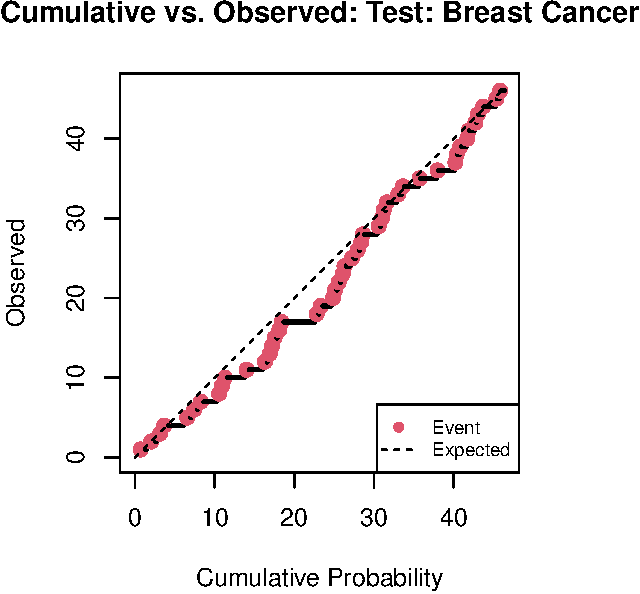
\includegraphics{BreastCancerRoyAltman_files/figure-latex/unnamed-chunk-9-1.pdf}
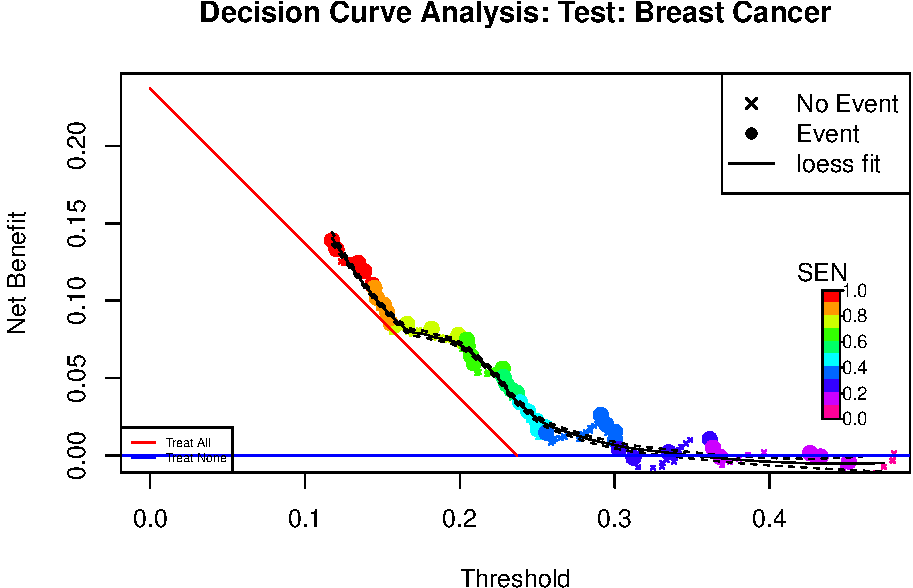
\includegraphics{BreastCancerRoyAltman_files/figure-latex/unnamed-chunk-9-2.pdf}
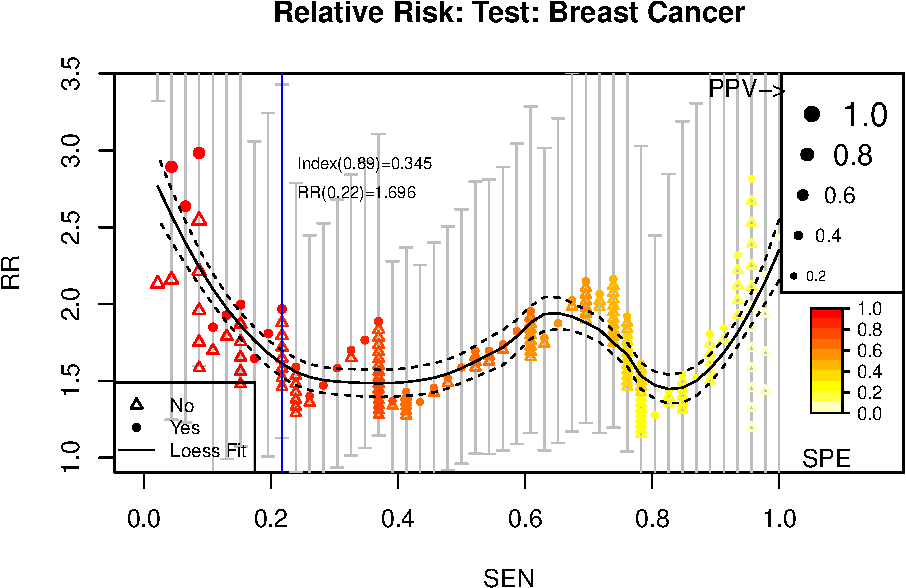
\includegraphics{BreastCancerRoyAltman_files/figure-latex/unnamed-chunk-9-3.pdf}
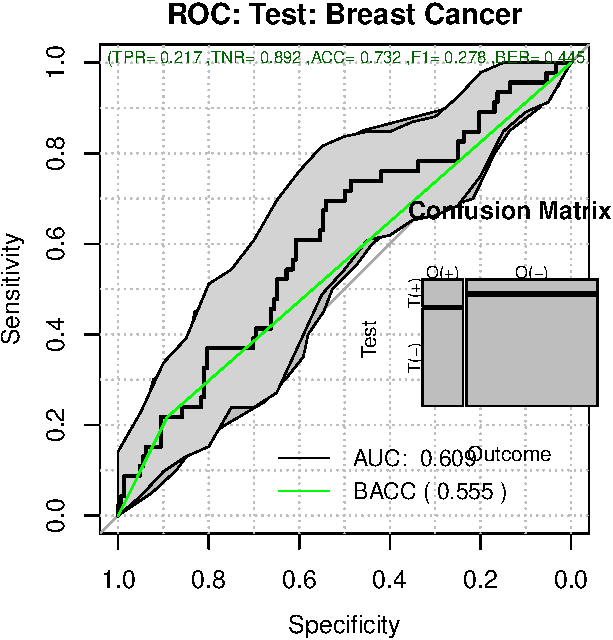
\includegraphics{BreastCancerRoyAltman_files/figure-latex/unnamed-chunk-9-4.pdf}
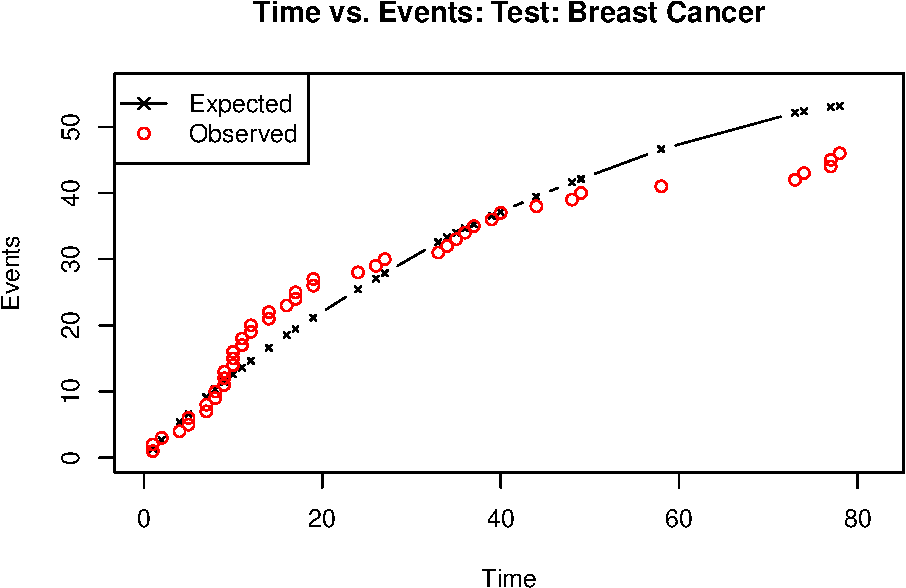
\includegraphics{BreastCancerRoyAltman_files/figure-latex/unnamed-chunk-9-5.pdf}
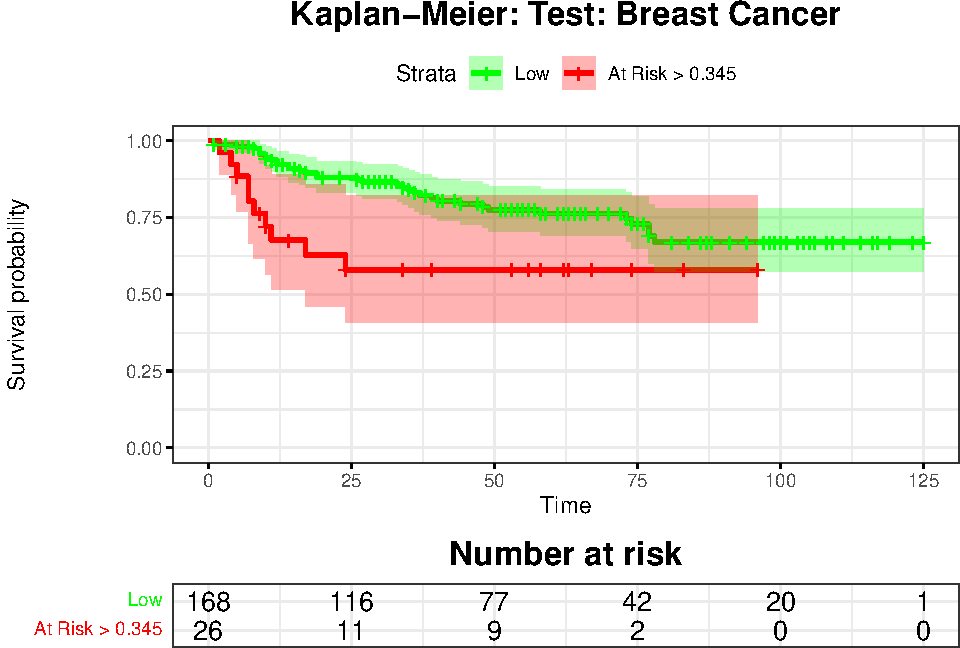
\includegraphics{BreastCancerRoyAltman_files/figure-latex/unnamed-chunk-9-6.pdf}

\hypertarget{time-to-event-after-calibration}{%
\subsubsection{Time to event after
calibration}\label{time-to-event-after-calibration}}

\begin{Shaded}
\begin{Highlighting}[]
\NormalTok{toinclude }\OtherTok{\textless{}{-}}\NormalTok{ dataBrestCancerTrain}\SpecialCharTok{$}\NormalTok{status}\SpecialCharTok{==}\DecValTok{1}
\NormalTok{obstiemToEvent }\OtherTok{\textless{}{-}}\NormalTok{ dataBrestCancerTrain}\SpecialCharTok{$}\NormalTok{time}
\NormalTok{timetoEvent }\OtherTok{\textless{}{-}} \FunctionTok{meanTimeToEvent}\NormalTok{(rdata[,}\DecValTok{2}\NormalTok{],timeinterval)}
\NormalTok{tmax}\OtherTok{\textless{}{-}}\FunctionTok{max}\NormalTok{(}\FunctionTok{c}\NormalTok{(obstiemToEvent,timetoEvent))}
\NormalTok{tmin}\OtherTok{\textless{}{-}}\FunctionTok{min}\NormalTok{(}\FunctionTok{c}\NormalTok{(obstiemToEvent,timetoEvent))}
\NormalTok{lnotime }\OtherTok{\textless{}{-}} \FunctionTok{log}\NormalTok{(obstiemToEvent[toinclude])}
\NormalTok{lnetime }\OtherTok{\textless{}{-}} \FunctionTok{log}\NormalTok{(timetoEvent[toinclude])}
\NormalTok{lmfit }\OtherTok{\textless{}{-}} \FunctionTok{lm}\NormalTok{(lnotime}\SpecialCharTok{\textasciitilde{}}\DecValTok{0}\SpecialCharTok{+}\NormalTok{lnetime)}
\NormalTok{sm }\OtherTok{\textless{}{-}} \FunctionTok{summary}\NormalTok{(lmfit)}
\NormalTok{pander}\SpecialCharTok{::}\FunctionTok{pander}\NormalTok{(sm)}
\end{Highlighting}
\end{Shaded}

\begin{longtable}[]{@{}
  >{\centering\arraybackslash}p{(\columnwidth - 8\tabcolsep) * \real{0.1944}}
  >{\centering\arraybackslash}p{(\columnwidth - 8\tabcolsep) * \real{0.1528}}
  >{\centering\arraybackslash}p{(\columnwidth - 8\tabcolsep) * \real{0.1806}}
  >{\centering\arraybackslash}p{(\columnwidth - 8\tabcolsep) * \real{0.1389}}
  >{\centering\arraybackslash}p{(\columnwidth - 8\tabcolsep) * \real{0.1667}}@{}}
\toprule()
\begin{minipage}[b]{\linewidth}\centering
~
\end{minipage} & \begin{minipage}[b]{\linewidth}\centering
Estimate
\end{minipage} & \begin{minipage}[b]{\linewidth}\centering
Std. Error
\end{minipage} & \begin{minipage}[b]{\linewidth}\centering
t value
\end{minipage} & \begin{minipage}[b]{\linewidth}\centering
Pr(\textgreater\textbar t\textbar)
\end{minipage} \\
\midrule()
\endhead
\textbf{lnetime} & 0.585 & 0.0139 & 42.1 & 3.04e-257 \\
\bottomrule()
\end{longtable}

\begin{longtable}[]{@{}
  >{\centering\arraybackslash}p{(\columnwidth - 6\tabcolsep) * \real{0.2083}}
  >{\centering\arraybackslash}p{(\columnwidth - 6\tabcolsep) * \real{0.3056}}
  >{\centering\arraybackslash}p{(\columnwidth - 6\tabcolsep) * \real{0.1111}}
  >{\centering\arraybackslash}p{(\columnwidth - 6\tabcolsep) * \real{0.2361}}@{}}
\caption{Fitting linear model: lnotime \textasciitilde{} 0 +
lnetime}\tabularnewline
\toprule()
\begin{minipage}[b]{\linewidth}\centering
Observations
\end{minipage} & \begin{minipage}[b]{\linewidth}\centering
Residual Std. Error
\end{minipage} & \begin{minipage}[b]{\linewidth}\centering
\(R^2\)
\end{minipage} & \begin{minipage}[b]{\linewidth}\centering
Adjusted \(R^2\)
\end{minipage} \\
\midrule()
\endfirsthead
\toprule()
\begin{minipage}[b]{\linewidth}\centering
Observations
\end{minipage} & \begin{minipage}[b]{\linewidth}\centering
Residual Std. Error
\end{minipage} & \begin{minipage}[b]{\linewidth}\centering
\(R^2\)
\end{minipage} & \begin{minipage}[b]{\linewidth}\centering
Adjusted \(R^2\)
\end{minipage} \\
\midrule()
\endhead
1518 & 0.839 & 0.539 & 0.539 \\
\bottomrule()
\end{longtable}

\begin{Shaded}
\begin{Highlighting}[]
\FunctionTok{plot}\NormalTok{(timetoEvent,obstiemToEvent,}
     \AttributeTok{col=}\DecValTok{1}\SpecialCharTok{+}\NormalTok{rdata[,}\DecValTok{1}\NormalTok{],}
     \AttributeTok{xlab=}\StringTok{"Expected time"}\NormalTok{,}
     \AttributeTok{ylab=}\StringTok{"Observed time"}\NormalTok{,}
     \AttributeTok{main=}\StringTok{"Expected vs. Observed"}\NormalTok{,}
     \AttributeTok{xlim=}\FunctionTok{c}\NormalTok{(tmin,tmax),}
     \AttributeTok{ylim=}\FunctionTok{c}\NormalTok{(tmin,tmax),}
     \AttributeTok{log=}\StringTok{"xy"}\NormalTok{)}
\FunctionTok{lines}\NormalTok{(}\AttributeTok{x=}\FunctionTok{c}\NormalTok{(tmin,tmax),}\AttributeTok{y=}\NormalTok{lmfit}\SpecialCharTok{$}\NormalTok{coefficients}\SpecialCharTok{*}\FunctionTok{c}\NormalTok{(tmin,tmax),}\AttributeTok{lty=}\DecValTok{1}\NormalTok{,}\AttributeTok{col=}\StringTok{"blue"}\NormalTok{)}
\NormalTok{txt }\OtherTok{\textless{}{-}} \FunctionTok{bquote}\NormalTok{(}\FunctionTok{paste}\NormalTok{(R}\SpecialCharTok{\^{}}\DecValTok{2} \SpecialCharTok{==}\NormalTok{ .(}\FunctionTok{round}\NormalTok{(sm}\SpecialCharTok{$}\NormalTok{r.squared,}\DecValTok{3}\NormalTok{))))}
\FunctionTok{text}\NormalTok{(tmin}\FloatTok{+0.005}\SpecialCharTok{*}\NormalTok{(tmax}\SpecialCharTok{{-}}\NormalTok{tmin),tmax,txt,}\AttributeTok{cex=}\FloatTok{0.7}\NormalTok{)}
\FunctionTok{text}\NormalTok{(tmin}\FloatTok{+0.015}\SpecialCharTok{*}\NormalTok{(tmax}\SpecialCharTok{{-}}\NormalTok{tmin),tmax,}\FunctionTok{sprintf}\NormalTok{(}\StringTok{"Slope=\%4.3f"}\NormalTok{,sm}\SpecialCharTok{$}\NormalTok{coefficients[}\DecValTok{1}\NormalTok{]),}\AttributeTok{cex=}\FloatTok{0.7}\NormalTok{)}
\FunctionTok{legend}\NormalTok{(}\StringTok{"bottomright"}\NormalTok{,}\AttributeTok{legend=}\FunctionTok{c}\NormalTok{(}\StringTok{"No Event"}\NormalTok{,}\StringTok{"Event"}\NormalTok{,}\StringTok{"Linear fit"}\NormalTok{),}
             \AttributeTok{pch=}\FunctionTok{c}\NormalTok{(}\DecValTok{1}\NormalTok{,}\DecValTok{1}\NormalTok{,}\SpecialCharTok{{-}}\DecValTok{1}\NormalTok{),}
             \AttributeTok{col=}\FunctionTok{c}\NormalTok{(}\DecValTok{1}\NormalTok{,}\DecValTok{2}\NormalTok{,}\StringTok{"blue"}\NormalTok{),}
             \AttributeTok{lty=}\FunctionTok{c}\NormalTok{(}\SpecialCharTok{{-}}\DecValTok{1}\NormalTok{,}\SpecialCharTok{{-}}\DecValTok{1}\NormalTok{,}\DecValTok{1}\NormalTok{)}
\NormalTok{             )}
\end{Highlighting}
\end{Shaded}

\includegraphics{BreastCancerRoyAltman_files/figure-latex/unnamed-chunk-10-1.pdf}

\begin{Shaded}
\begin{Highlighting}[]
\NormalTok{MADerror2 }\OtherTok{\textless{}{-}} \FunctionTok{mean}\NormalTok{(}\FunctionTok{abs}\NormalTok{(timetoEvent[toinclude]}\SpecialCharTok{{-}}\NormalTok{obstiemToEvent[toinclude]))}
\NormalTok{pander}\SpecialCharTok{::}\FunctionTok{pander}\NormalTok{(MADerror2)}
\end{Highlighting}
\end{Shaded}

\emph{2.65}

\hypertarget{by-risk-categories-1}{%
\subsubsection{By Risk Categories}\label{by-risk-categories-1}}

\begin{Shaded}
\begin{Highlighting}[]
\NormalTok{hazards }\OtherTok{\textless{}{-}} \SpecialCharTok{{-}}\FunctionTok{log}\NormalTok{(}\FloatTok{1.0}\SpecialCharTok{{-}}\NormalTok{rdata[,}\DecValTok{2}\NormalTok{])}\SpecialCharTok{*}\NormalTok{dataBrestCancerTrain}\SpecialCharTok{$}\NormalTok{time}\SpecialCharTok{/}\NormalTok{calprob}\SpecialCharTok{$}\NormalTok{timeInterval}
\NormalTok{procat }\OtherTok{\textless{}{-}} \FunctionTok{floor}\NormalTok{(}\DecValTok{5}\SpecialCharTok{*}\NormalTok{rdata[,}\DecValTok{2}\NormalTok{])}
\NormalTok{values }\OtherTok{\textless{}{-}} \FunctionTok{unique}\NormalTok{(procat)}
\NormalTok{values }\OtherTok{\textless{}{-}}\NormalTok{ values[}\FunctionTok{order}\NormalTok{(values)]}
\NormalTok{obs }\OtherTok{\textless{}{-}} \FunctionTok{numeric}\NormalTok{()}
\NormalTok{expected }\OtherTok{\textless{}{-}} \FunctionTok{numeric}\NormalTok{()}
\NormalTok{lci }\OtherTok{\textless{}{-}} \FunctionTok{numeric}\NormalTok{()}
\NormalTok{uci }\OtherTok{\textless{}{-}} \FunctionTok{numeric}\NormalTok{()}
\ControlFlowTok{for}\NormalTok{ (ct }\ControlFlowTok{in}\NormalTok{ values)}
\NormalTok{\{}
\NormalTok{  totobs }\OtherTok{\textless{}{-}} \FunctionTok{sum}\NormalTok{(rdata[procat}\SpecialCharTok{==}\NormalTok{ct,}\DecValTok{1}\NormalTok{])}
\NormalTok{  obs }\OtherTok{\textless{}{-}}\FunctionTok{c}\NormalTok{(obs,totobs)}
\NormalTok{  expected }\OtherTok{\textless{}{-}} \FunctionTok{c}\NormalTok{(expected,}\FunctionTok{sum}\NormalTok{(hazards[procat}\SpecialCharTok{==}\NormalTok{ct]))}
\NormalTok{  pt }\OtherTok{\textless{}{-}} \FunctionTok{poisson.test}\NormalTok{(totobs,}\DecValTok{1}\NormalTok{)}
\NormalTok{  lci }\OtherTok{\textless{}{-}} \FunctionTok{c}\NormalTok{(lci,pt}\SpecialCharTok{$}\NormalTok{conf.int[}\DecValTok{1}\NormalTok{])}
\NormalTok{  uci }\OtherTok{\textless{}{-}} \FunctionTok{c}\NormalTok{(uci,pt}\SpecialCharTok{$}\NormalTok{conf.int[}\DecValTok{2}\NormalTok{])}

\NormalTok{\}}
\NormalTok{maxx }\OtherTok{\textless{}{-}} \FunctionTok{max}\NormalTok{(}\FunctionTok{c}\NormalTok{(obs,expected))}
\NormalTok{minx }\OtherTok{\textless{}{-}} \FunctionTok{min}\NormalTok{(}\FunctionTok{c}\NormalTok{(obs,expected))}

\FunctionTok{plot}\NormalTok{(expected,obs,}
     \AttributeTok{xlim=}\FunctionTok{c}\NormalTok{(minx,maxx),}
     \AttributeTok{ylim=}\FunctionTok{c}\NormalTok{(minx,maxx),}
     \AttributeTok{main=}\StringTok{"Expected vs Observed"}\NormalTok{,}
     \AttributeTok{ylab=}\StringTok{"Observed"}\NormalTok{,}
     \AttributeTok{xlab=}\StringTok{"Expected"}\NormalTok{,}
     \AttributeTok{col=}\DecValTok{1}\SpecialCharTok{+}\NormalTok{values)}

\FunctionTok{errbar}\NormalTok{(expected,obs,lci,uci,}\AttributeTok{add=}\ConstantTok{TRUE}\NormalTok{,}\AttributeTok{pch=}\DecValTok{0}\NormalTok{,}\AttributeTok{errbar.col=}\DecValTok{1}\SpecialCharTok{+}\NormalTok{values,}\AttributeTok{cex=}\FloatTok{0.25}\NormalTok{)}
\FunctionTok{lines}\NormalTok{(}\AttributeTok{x=}\FunctionTok{c}\NormalTok{(}\DecValTok{0}\NormalTok{,maxx),}\AttributeTok{y=}\FunctionTok{c}\NormalTok{(}\DecValTok{0}\NormalTok{,maxx),}\AttributeTok{lty=}\DecValTok{2}\NormalTok{)}
\end{Highlighting}
\end{Shaded}

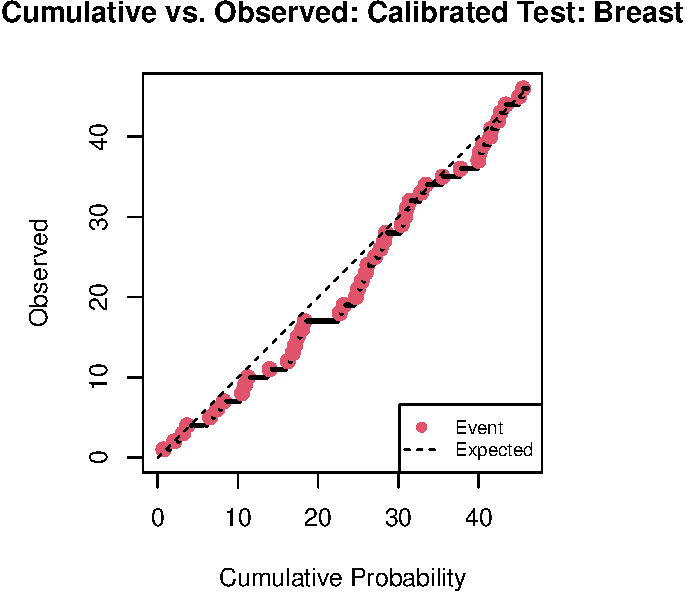
\includegraphics{BreastCancerRoyAltman_files/figure-latex/unnamed-chunk-11-1.pdf}

\hypertarget{calibrated-train-performance}{%
\subsubsection{Calibrated Train
Performance}\label{calibrated-train-performance}}

\begin{Shaded}
\begin{Highlighting}[]
\NormalTok{pander}\SpecialCharTok{::}\FunctionTok{pander}\NormalTok{(}\FunctionTok{t}\NormalTok{(rrAnalysisTrain}\SpecialCharTok{$}\NormalTok{keyPoints),}\AttributeTok{caption=}\StringTok{"Threshold values"}\NormalTok{)}
\end{Highlighting}
\end{Shaded}

\begin{longtable}[]{@{}
  >{\centering\arraybackslash}p{(\columnwidth - 12\tabcolsep) * \real{0.2237}}
  >{\centering\arraybackslash}p{(\columnwidth - 12\tabcolsep) * \real{0.1184}}
  >{\centering\arraybackslash}p{(\columnwidth - 12\tabcolsep) * \real{0.1053}}
  >{\centering\arraybackslash}p{(\columnwidth - 12\tabcolsep) * \real{0.1579}}
  >{\centering\arraybackslash}p{(\columnwidth - 12\tabcolsep) * \real{0.1316}}
  >{\centering\arraybackslash}p{(\columnwidth - 12\tabcolsep) * \real{0.1316}}
  >{\centering\arraybackslash}p{(\columnwidth - 12\tabcolsep) * \real{0.1316}}@{}}
\caption{Threshold values}\tabularnewline
\toprule()
\begin{minipage}[b]{\linewidth}\centering
~
\end{minipage} & \begin{minipage}[b]{\linewidth}\centering
@:0.9
\end{minipage} & \begin{minipage}[b]{\linewidth}\centering
@:0.8
\end{minipage} & \begin{minipage}[b]{\linewidth}\centering
@MAX\_BACC
\end{minipage} & \begin{minipage}[b]{\linewidth}\centering
@MAX\_RR
\end{minipage} & \begin{minipage}[b]{\linewidth}\centering
@SPE100
\end{minipage} & \begin{minipage}[b]{\linewidth}\centering
p(0.5)
\end{minipage} \\
\midrule()
\endfirsthead
\toprule()
\begin{minipage}[b]{\linewidth}\centering
~
\end{minipage} & \begin{minipage}[b]{\linewidth}\centering
@:0.9
\end{minipage} & \begin{minipage}[b]{\linewidth}\centering
@:0.8
\end{minipage} & \begin{minipage}[b]{\linewidth}\centering
@MAX\_BACC
\end{minipage} & \begin{minipage}[b]{\linewidth}\centering
@MAX\_RR
\end{minipage} & \begin{minipage}[b]{\linewidth}\centering
@SPE100
\end{minipage} & \begin{minipage}[b]{\linewidth}\centering
p(0.5)
\end{minipage} \\
\midrule()
\endhead
\textbf{Thr} & 0.6383 & 0.558 & 0.472 & 0.329 & 0.28808 & 0.499 \\
\textbf{RR} & 1.6904 & 1.713 & 1.799 & 2.376 & 1.00000 & 1.741 \\
\textbf{RR\_LCI} & 1.5860 & 1.603 & 1.666 & 1.869 & 0.00000 & 1.620 \\
\textbf{RR\_UCI} & 1.8018 & 1.830 & 1.942 & 3.019 & 0.00000 & 1.872 \\
\textbf{SEN} & 0.2991 & 0.462 & 0.644 & 0.965 & 1.00000 & 0.589 \\
\textbf{SPE} & 0.8996 & 0.798 & 0.646 & 0.125 & 0.00137 & 0.691 \\
\textbf{BACC} & 0.5993 & 0.630 & 0.645 & 0.545 & 0.50068 & 0.640 \\
\textbf{NetBenefit} & 0.0653 & 0.111 & 0.173 & 0.281 & 0.31069 &
0.149 \\
\bottomrule()
\end{longtable}

\begin{Shaded}
\begin{Highlighting}[]
\NormalTok{pander}\SpecialCharTok{::}\FunctionTok{pander}\NormalTok{(}\FunctionTok{t}\NormalTok{(rrAnalysisTrain}\SpecialCharTok{$}\NormalTok{OERatio}\SpecialCharTok{$}\NormalTok{estimate),}\AttributeTok{caption=}\StringTok{"O/E Ratio"}\NormalTok{)}
\end{Highlighting}
\end{Shaded}

\begin{longtable}[]{@{}
  >{\centering\arraybackslash}p{(\columnwidth - 6\tabcolsep) * \real{0.1111}}
  >{\centering\arraybackslash}p{(\columnwidth - 6\tabcolsep) * \real{0.1111}}
  >{\centering\arraybackslash}p{(\columnwidth - 6\tabcolsep) * \real{0.1111}}
  >{\centering\arraybackslash}p{(\columnwidth - 6\tabcolsep) * \real{0.1528}}@{}}
\caption{O/E Ratio}\tabularnewline
\toprule()
\begin{minipage}[b]{\linewidth}\centering
O/E
\end{minipage} & \begin{minipage}[b]{\linewidth}\centering
Low
\end{minipage} & \begin{minipage}[b]{\linewidth}\centering
Upper
\end{minipage} & \begin{minipage}[b]{\linewidth}\centering
p.value
\end{minipage} \\
\midrule()
\endfirsthead
\toprule()
\begin{minipage}[b]{\linewidth}\centering
O/E
\end{minipage} & \begin{minipage}[b]{\linewidth}\centering
Low
\end{minipage} & \begin{minipage}[b]{\linewidth}\centering
Upper
\end{minipage} & \begin{minipage}[b]{\linewidth}\centering
p.value
\end{minipage} \\
\midrule()
\endhead
0.896 & 0.852 & 0.942 & 1.44e-05 \\
\bottomrule()
\end{longtable}

\begin{Shaded}
\begin{Highlighting}[]
\NormalTok{pander}\SpecialCharTok{::}\FunctionTok{pander}\NormalTok{(}\FunctionTok{t}\NormalTok{(rrAnalysisTrain}\SpecialCharTok{$}\NormalTok{OE95ci),}\AttributeTok{caption=}\StringTok{"O/E Mean"}\NormalTok{)}
\end{Highlighting}
\end{Shaded}

\begin{longtable}[]{@{}
  >{\centering\arraybackslash}p{(\columnwidth - 6\tabcolsep) * \real{0.1111}}
  >{\centering\arraybackslash}p{(\columnwidth - 6\tabcolsep) * \real{0.1111}}
  >{\centering\arraybackslash}p{(\columnwidth - 6\tabcolsep) * \real{0.1111}}
  >{\centering\arraybackslash}p{(\columnwidth - 6\tabcolsep) * \real{0.1111}}@{}}
\caption{O/E Mean}\tabularnewline
\toprule()
\begin{minipage}[b]{\linewidth}\centering
mean
\end{minipage} & \begin{minipage}[b]{\linewidth}\centering
50\%
\end{minipage} & \begin{minipage}[b]{\linewidth}\centering
2.5\%
\end{minipage} & \begin{minipage}[b]{\linewidth}\centering
97.5\%
\end{minipage} \\
\midrule()
\endfirsthead
\toprule()
\begin{minipage}[b]{\linewidth}\centering
mean
\end{minipage} & \begin{minipage}[b]{\linewidth}\centering
50\%
\end{minipage} & \begin{minipage}[b]{\linewidth}\centering
2.5\%
\end{minipage} & \begin{minipage}[b]{\linewidth}\centering
97.5\%
\end{minipage} \\
\midrule()
\endhead
0.988 & 0.989 & 0.982 & 0.995 \\
\bottomrule()
\end{longtable}

\begin{Shaded}
\begin{Highlighting}[]
\NormalTok{pander}\SpecialCharTok{::}\FunctionTok{pander}\NormalTok{(}\FunctionTok{t}\NormalTok{(rrAnalysisTrain}\SpecialCharTok{$}\NormalTok{OAcum95ci),}\AttributeTok{caption=}\StringTok{"O/Acum Mean"}\NormalTok{)}
\end{Highlighting}
\end{Shaded}

\begin{longtable}[]{@{}
  >{\centering\arraybackslash}p{(\columnwidth - 6\tabcolsep) * \real{0.0972}}
  >{\centering\arraybackslash}p{(\columnwidth - 6\tabcolsep) * \real{0.0972}}
  >{\centering\arraybackslash}p{(\columnwidth - 6\tabcolsep) * \real{0.0972}}
  >{\centering\arraybackslash}p{(\columnwidth - 6\tabcolsep) * \real{0.1111}}@{}}
\caption{O/Acum Mean}\tabularnewline
\toprule()
\begin{minipage}[b]{\linewidth}\centering
mean
\end{minipage} & \begin{minipage}[b]{\linewidth}\centering
50\%
\end{minipage} & \begin{minipage}[b]{\linewidth}\centering
2.5\%
\end{minipage} & \begin{minipage}[b]{\linewidth}\centering
97.5\%
\end{minipage} \\
\midrule()
\endfirsthead
\toprule()
\begin{minipage}[b]{\linewidth}\centering
mean
\end{minipage} & \begin{minipage}[b]{\linewidth}\centering
50\%
\end{minipage} & \begin{minipage}[b]{\linewidth}\centering
2.5\%
\end{minipage} & \begin{minipage}[b]{\linewidth}\centering
97.5\%
\end{minipage} \\
\midrule()
\endhead
1.03 & 1.03 & 1.03 & 1.03 \\
\bottomrule()
\end{longtable}

\begin{Shaded}
\begin{Highlighting}[]
\NormalTok{pander}\SpecialCharTok{::}\FunctionTok{pander}\NormalTok{(rrAnalysisTrain}\SpecialCharTok{$}\NormalTok{c.index}\SpecialCharTok{$}\NormalTok{cstatCI,}\AttributeTok{caption=}\StringTok{"C. Index"}\NormalTok{)}
\end{Highlighting}
\end{Shaded}

\begin{longtable}[]{@{}
  >{\centering\arraybackslash}p{(\columnwidth - 6\tabcolsep) * \real{0.2083}}
  >{\centering\arraybackslash}p{(\columnwidth - 6\tabcolsep) * \real{0.1250}}
  >{\centering\arraybackslash}p{(\columnwidth - 6\tabcolsep) * \real{0.1111}}
  >{\centering\arraybackslash}p{(\columnwidth - 6\tabcolsep) * \real{0.1111}}@{}}
\toprule()
\begin{minipage}[b]{\linewidth}\centering
mean.C Index
\end{minipage} & \begin{minipage}[b]{\linewidth}\centering
median
\end{minipage} & \begin{minipage}[b]{\linewidth}\centering
lower
\end{minipage} & \begin{minipage}[b]{\linewidth}\centering
upper
\end{minipage} \\
\midrule()
\endhead
0.676 & 0.676 & 0.662 & 0.69 \\
\bottomrule()
\end{longtable}

\begin{Shaded}
\begin{Highlighting}[]
\NormalTok{pander}\SpecialCharTok{::}\FunctionTok{pander}\NormalTok{(}\FunctionTok{t}\NormalTok{(rrAnalysisTrain}\SpecialCharTok{$}\NormalTok{ROCAnalysis}\SpecialCharTok{$}\NormalTok{aucs),}\AttributeTok{caption=}\StringTok{"ROC AUC"}\NormalTok{)}
\end{Highlighting}
\end{Shaded}

\begin{longtable}[]{@{}
  >{\centering\arraybackslash}p{(\columnwidth - 4\tabcolsep) * \real{0.1111}}
  >{\centering\arraybackslash}p{(\columnwidth - 4\tabcolsep) * \real{0.1111}}
  >{\centering\arraybackslash}p{(\columnwidth - 4\tabcolsep) * \real{0.1111}}@{}}
\caption{ROC AUC}\tabularnewline
\toprule()
\begin{minipage}[b]{\linewidth}\centering
est
\end{minipage} & \begin{minipage}[b]{\linewidth}\centering
lower
\end{minipage} & \begin{minipage}[b]{\linewidth}\centering
upper
\end{minipage} \\
\midrule()
\endfirsthead
\toprule()
\begin{minipage}[b]{\linewidth}\centering
est
\end{minipage} & \begin{minipage}[b]{\linewidth}\centering
lower
\end{minipage} & \begin{minipage}[b]{\linewidth}\centering
upper
\end{minipage} \\
\midrule()
\endhead
0.694 & 0.675 & 0.713 \\
\bottomrule()
\end{longtable}

\begin{Shaded}
\begin{Highlighting}[]
\NormalTok{pander}\SpecialCharTok{::}\FunctionTok{pander}\NormalTok{((rrAnalysisTrain}\SpecialCharTok{$}\NormalTok{ROCAnalysis}\SpecialCharTok{$}\NormalTok{sensitivity),}\AttributeTok{caption=}\StringTok{"Sensitivity"}\NormalTok{)}
\end{Highlighting}
\end{Shaded}

\begin{longtable}[]{@{}
  >{\centering\arraybackslash}p{(\columnwidth - 4\tabcolsep) * \real{0.1111}}
  >{\centering\arraybackslash}p{(\columnwidth - 4\tabcolsep) * \real{0.1111}}
  >{\centering\arraybackslash}p{(\columnwidth - 4\tabcolsep) * \real{0.1111}}@{}}
\caption{Sensitivity}\tabularnewline
\toprule()
\begin{minipage}[b]{\linewidth}\centering
est
\end{minipage} & \begin{minipage}[b]{\linewidth}\centering
lower
\end{minipage} & \begin{minipage}[b]{\linewidth}\centering
upper
\end{minipage} \\
\midrule()
\endfirsthead
\toprule()
\begin{minipage}[b]{\linewidth}\centering
est
\end{minipage} & \begin{minipage}[b]{\linewidth}\centering
lower
\end{minipage} & \begin{minipage}[b]{\linewidth}\centering
upper
\end{minipage} \\
\midrule()
\endhead
0.299 & 0.276 & 0.323 \\
\bottomrule()
\end{longtable}

\begin{Shaded}
\begin{Highlighting}[]
\NormalTok{pander}\SpecialCharTok{::}\FunctionTok{pander}\NormalTok{((rrAnalysisTrain}\SpecialCharTok{$}\NormalTok{ROCAnalysis}\SpecialCharTok{$}\NormalTok{specificity),}\AttributeTok{caption=}\StringTok{"Specificity"}\NormalTok{)}
\end{Highlighting}
\end{Shaded}

\begin{longtable}[]{@{}
  >{\centering\arraybackslash}p{(\columnwidth - 4\tabcolsep) * \real{0.0833}}
  >{\centering\arraybackslash}p{(\columnwidth - 4\tabcolsep) * \real{0.1111}}
  >{\centering\arraybackslash}p{(\columnwidth - 4\tabcolsep) * \real{0.1111}}@{}}
\caption{Specificity}\tabularnewline
\toprule()
\begin{minipage}[b]{\linewidth}\centering
est
\end{minipage} & \begin{minipage}[b]{\linewidth}\centering
lower
\end{minipage} & \begin{minipage}[b]{\linewidth}\centering
upper
\end{minipage} \\
\midrule()
\endfirsthead
\toprule()
\begin{minipage}[b]{\linewidth}\centering
est
\end{minipage} & \begin{minipage}[b]{\linewidth}\centering
lower
\end{minipage} & \begin{minipage}[b]{\linewidth}\centering
upper
\end{minipage} \\
\midrule()
\endhead
0.9 & 0.883 & 0.915 \\
\bottomrule()
\end{longtable}

\begin{Shaded}
\begin{Highlighting}[]
\NormalTok{pander}\SpecialCharTok{::}\FunctionTok{pander}\NormalTok{(}\FunctionTok{t}\NormalTok{(rrAnalysisTrain}\SpecialCharTok{$}\NormalTok{thr\_atP),}\AttributeTok{caption=}\StringTok{"Probability Thresholds"}\NormalTok{)}
\end{Highlighting}
\end{Shaded}

\begin{longtable}[]{@{}
  >{\centering\arraybackslash}p{(\columnwidth - 2\tabcolsep) * \real{0.1111}}
  >{\centering\arraybackslash}p{(\columnwidth - 2\tabcolsep) * \real{0.1111}}@{}}
\caption{Probability Thresholds}\tabularnewline
\toprule()
\begin{minipage}[b]{\linewidth}\centering
90\%
\end{minipage} & \begin{minipage}[b]{\linewidth}\centering
80\%
\end{minipage} \\
\midrule()
\endfirsthead
\toprule()
\begin{minipage}[b]{\linewidth}\centering
90\%
\end{minipage} & \begin{minipage}[b]{\linewidth}\centering
80\%
\end{minipage} \\
\midrule()
\endhead
0.638 & 0.558 \\
\bottomrule()
\end{longtable}

\begin{Shaded}
\begin{Highlighting}[]
\NormalTok{pander}\SpecialCharTok{::}\FunctionTok{pander}\NormalTok{(rrAnalysisTrain}\SpecialCharTok{$}\NormalTok{surdif,}\AttributeTok{caption=}\StringTok{"Logrank test"}\NormalTok{)}
\end{Highlighting}
\end{Shaded}

\begin{longtable}[]{@{}
  >{\centering\arraybackslash}p{(\columnwidth - 10\tabcolsep) * \real{0.1944}}
  >{\centering\arraybackslash}p{(\columnwidth - 10\tabcolsep) * \real{0.0972}}
  >{\centering\arraybackslash}p{(\columnwidth - 10\tabcolsep) * \real{0.1528}}
  >{\centering\arraybackslash}p{(\columnwidth - 10\tabcolsep) * \real{0.1528}}
  >{\centering\arraybackslash}p{(\columnwidth - 10\tabcolsep) * \real{0.1667}}
  >{\centering\arraybackslash}p{(\columnwidth - 10\tabcolsep) * \real{0.1667}}@{}}
\caption{Logrank test Chisq = 465.079317 on 2 degrees of freedom, p =
0.000000}\tabularnewline
\toprule()
\begin{minipage}[b]{\linewidth}\centering
~
\end{minipage} & \begin{minipage}[b]{\linewidth}\centering
N
\end{minipage} & \begin{minipage}[b]{\linewidth}\centering
Observed
\end{minipage} & \begin{minipage}[b]{\linewidth}\centering
Expected
\end{minipage} & \begin{minipage}[b]{\linewidth}\centering
(O-E)\^{}2/E
\end{minipage} & \begin{minipage}[b]{\linewidth}\centering
(O-E)\^{}2/V
\end{minipage} \\
\midrule()
\endfirsthead
\toprule()
\begin{minipage}[b]{\linewidth}\centering
~
\end{minipage} & \begin{minipage}[b]{\linewidth}\centering
N
\end{minipage} & \begin{minipage}[b]{\linewidth}\centering
Observed
\end{minipage} & \begin{minipage}[b]{\linewidth}\centering
Expected
\end{minipage} & \begin{minipage}[b]{\linewidth}\centering
(O-E)\^{}2/E
\end{minipage} & \begin{minipage}[b]{\linewidth}\centering
(O-E)\^{}2/V
\end{minipage} \\
\midrule()
\endhead
\textbf{class=0} & 1985 & 816 & 1144 & 93.9 & 385.7 \\
\textbf{class=1} & 396 & 248 & 177 & 28.0 & 31.8 \\
\textbf{class=2} & 601 & 454 & 197 & 336.3 & 391.3 \\
\bottomrule()
\end{longtable}

\hypertarget{performance-on-the-external-data-set}{%
\subsection{Performance on the external data
set}\label{performance-on-the-external-data-set}}

\begin{Shaded}
\begin{Highlighting}[]
\NormalTok{index }\OtherTok{\textless{}{-}} \FunctionTok{predict}\NormalTok{(ml,dataBrestCancerTest)}
\NormalTok{pp }\OtherTok{\textless{}{-}} \FunctionTok{predictionStats\_binary}\NormalTok{(}\FunctionTok{cbind}\NormalTok{(dataBrestCancerTest}\SpecialCharTok{$}\NormalTok{status,index),}\AttributeTok{plotname=}\StringTok{"Breast Cancer"}\NormalTok{)}
\end{Highlighting}
\end{Shaded}

\includegraphics{BreastCancerRoyAltman_files/figure-latex/unnamed-chunk-13-1.pdf}

\begin{Shaded}
\begin{Highlighting}[]
\FunctionTok{par}\NormalTok{(op)}


\NormalTok{prob }\OtherTok{\textless{}{-}} \FunctionTok{ppoisGzero}\NormalTok{(index,h0)}
\NormalTok{rdata }\OtherTok{\textless{}{-}} \FunctionTok{cbind}\NormalTok{(dataBrestCancerTest}\SpecialCharTok{$}\NormalTok{status,prob)}
\NormalTok{rrCoxTestAnalysis }\OtherTok{\textless{}{-}} \FunctionTok{RRPlot}\NormalTok{(rdata,}\AttributeTok{atThr=}\NormalTok{rrAnalysisTrain}\SpecialCharTok{$}\NormalTok{thr\_atP,}
                     \AttributeTok{timetoEvent=}\NormalTok{dataBrestCancerTest}\SpecialCharTok{$}\NormalTok{time,}
                     \AttributeTok{title=}\StringTok{"Test: Breast Cancer"}\NormalTok{,}
                     \AttributeTok{ysurvlim=}\FunctionTok{c}\NormalTok{(}\FloatTok{0.00}\NormalTok{,}\FloatTok{1.0}\NormalTok{),}
                     \AttributeTok{riskTimeInterval=}\NormalTok{timeinterval)}
\end{Highlighting}
\end{Shaded}

\includegraphics{BreastCancerRoyAltman_files/figure-latex/unnamed-chunk-13-2.pdf}
\includegraphics{BreastCancerRoyAltman_files/figure-latex/unnamed-chunk-13-3.pdf}
\includegraphics{BreastCancerRoyAltman_files/figure-latex/unnamed-chunk-13-4.pdf}
\includegraphics{BreastCancerRoyAltman_files/figure-latex/unnamed-chunk-13-5.pdf}
\includegraphics{BreastCancerRoyAltman_files/figure-latex/unnamed-chunk-13-6.pdf}
\includegraphics{BreastCancerRoyAltman_files/figure-latex/unnamed-chunk-13-7.pdf}

\begin{Shaded}
\begin{Highlighting}[]
\FunctionTok{par}\NormalTok{(op)}
\end{Highlighting}
\end{Shaded}

\hypertarget{external-data-report}{%
\subsubsection{External Data Report}\label{external-data-report}}

\begin{Shaded}
\begin{Highlighting}[]
\NormalTok{pander}\SpecialCharTok{::}\FunctionTok{pander}\NormalTok{(}\FunctionTok{t}\NormalTok{(rrCoxTestAnalysis}\SpecialCharTok{$}\NormalTok{keyPoints),}\AttributeTok{caption=}\StringTok{"Threshold values"}\NormalTok{)}
\end{Highlighting}
\end{Shaded}

\begin{longtable}[]{@{}
  >{\centering\arraybackslash}p{(\columnwidth - 12\tabcolsep) * \real{0.2099}}
  >{\centering\arraybackslash}p{(\columnwidth - 12\tabcolsep) * \real{0.1235}}
  >{\centering\arraybackslash}p{(\columnwidth - 12\tabcolsep) * \real{0.1235}}
  >{\centering\arraybackslash}p{(\columnwidth - 12\tabcolsep) * \real{0.1481}}
  >{\centering\arraybackslash}p{(\columnwidth - 12\tabcolsep) * \real{0.1235}}
  >{\centering\arraybackslash}p{(\columnwidth - 12\tabcolsep) * \real{0.1358}}
  >{\centering\arraybackslash}p{(\columnwidth - 12\tabcolsep) * \real{0.1358}}@{}}
\caption{Threshold values}\tabularnewline
\toprule()
\begin{minipage}[b]{\linewidth}\centering
~
\end{minipage} & \begin{minipage}[b]{\linewidth}\centering
@:0.638
\end{minipage} & \begin{minipage}[b]{\linewidth}\centering
@:0.558
\end{minipage} & \begin{minipage}[b]{\linewidth}\centering
@MAX\_BACC
\end{minipage} & \begin{minipage}[b]{\linewidth}\centering
@MAX\_RR
\end{minipage} & \begin{minipage}[b]{\linewidth}\centering
@SPE100
\end{minipage} & \begin{minipage}[b]{\linewidth}\centering
p(0.5)
\end{minipage} \\
\midrule()
\endfirsthead
\toprule()
\begin{minipage}[b]{\linewidth}\centering
~
\end{minipage} & \begin{minipage}[b]{\linewidth}\centering
@:0.638
\end{minipage} & \begin{minipage}[b]{\linewidth}\centering
@:0.558
\end{minipage} & \begin{minipage}[b]{\linewidth}\centering
@MAX\_BACC
\end{minipage} & \begin{minipage}[b]{\linewidth}\centering
@MAX\_RR
\end{minipage} & \begin{minipage}[b]{\linewidth}\centering
@SPE100
\end{minipage} & \begin{minipage}[b]{\linewidth}\centering
p(0.5)
\end{minipage} \\
\midrule()
\endhead
\textbf{Thr} & 0.6378 & 0.5580 & 0.5899 & 0.342 & 2.75e-01 & 0.4992 \\
\textbf{RR} & 1.7994 & 1.6427 & 1.7581 & 3.279 & 2.64e+01 & 1.5739 \\
\textbf{RR\_LCI} & 1.5366 & 1.3951 & 1.4980 & 1.641 & 5.65e-02 &
1.3253 \\
\textbf{RR\_UCI} & 2.1071 & 1.9343 & 2.0632 & 6.552 & 1.23e+04 &
1.8691 \\
\textbf{SEN} & 0.3311 & 0.4515 & 0.4181 & 0.977 & 1.00e+00 & 0.5619 \\
\textbf{SPE} & 0.8734 & 0.7571 & 0.8088 & 0.111 & 1.55e-02 & 0.6382 \\
\textbf{BACC} & 0.6022 & 0.6043 & 0.6134 & 0.544 & 5.08e-01 & 0.6001 \\
\textbf{NetBenefit} & 0.0186 & 0.0238 & 0.0271 & 0.166 & 2.25e-01 &
0.0415 \\
\bottomrule()
\end{longtable}

\begin{Shaded}
\begin{Highlighting}[]
\NormalTok{pander}\SpecialCharTok{::}\FunctionTok{pander}\NormalTok{(}\FunctionTok{t}\NormalTok{(rrCoxTestAnalysis}\SpecialCharTok{$}\NormalTok{OERatio}\SpecialCharTok{$}\NormalTok{estimate),}\AttributeTok{caption=}\StringTok{"O/E Ratio"}\NormalTok{)}
\end{Highlighting}
\end{Shaded}

\begin{longtable}[]{@{}
  >{\centering\arraybackslash}p{(\columnwidth - 6\tabcolsep) * \real{0.0972}}
  >{\centering\arraybackslash}p{(\columnwidth - 6\tabcolsep) * \real{0.0972}}
  >{\centering\arraybackslash}p{(\columnwidth - 6\tabcolsep) * \real{0.1111}}
  >{\centering\arraybackslash}p{(\columnwidth - 6\tabcolsep) * \real{0.1528}}@{}}
\caption{O/E Ratio}\tabularnewline
\toprule()
\begin{minipage}[b]{\linewidth}\centering
O/E
\end{minipage} & \begin{minipage}[b]{\linewidth}\centering
Low
\end{minipage} & \begin{minipage}[b]{\linewidth}\centering
Upper
\end{minipage} & \begin{minipage}[b]{\linewidth}\centering
p.value
\end{minipage} \\
\midrule()
\endfirsthead
\toprule()
\begin{minipage}[b]{\linewidth}\centering
O/E
\end{minipage} & \begin{minipage}[b]{\linewidth}\centering
Low
\end{minipage} & \begin{minipage}[b]{\linewidth}\centering
Upper
\end{minipage} & \begin{minipage}[b]{\linewidth}\centering
p.value
\end{minipage} \\
\midrule()
\endhead
1.26 & 1.12 & 1.41 & 9.49e-05 \\
\bottomrule()
\end{longtable}

\begin{Shaded}
\begin{Highlighting}[]
\NormalTok{pander}\SpecialCharTok{::}\FunctionTok{pander}\NormalTok{(rrCoxTestAnalysis}\SpecialCharTok{$}\NormalTok{c.index,}\AttributeTok{caption=}\StringTok{"C. Index"}\NormalTok{)}
\end{Highlighting}
\end{Shaded}

\begin{itemize}
\item
  \textbf{C Index}: \emph{0.664}
\item
  \textbf{Dxy}: \emph{0.328}
\item
  \textbf{S.D.}: \emph{0.0311}
\item
  \textbf{n}: \emph{686}
\item
  \textbf{missing}: \emph{0}
\item
  \textbf{uncensored}: \emph{299}
\item
  \textbf{Relevant Pairs}: \emph{266144}
\item
  \textbf{Concordant}: \emph{176738}
\item
  \textbf{Uncertain}: \emph{203702}
\item
  \textbf{cstatCI}:

  \begin{longtable}[]{@{}
    >{\centering\arraybackslash}p{(\columnwidth - 6\tabcolsep) * \real{0.2083}}
    >{\centering\arraybackslash}p{(\columnwidth - 6\tabcolsep) * \real{0.1250}}
    >{\centering\arraybackslash}p{(\columnwidth - 6\tabcolsep) * \real{0.1111}}
    >{\centering\arraybackslash}p{(\columnwidth - 6\tabcolsep) * \real{0.1111}}@{}}
  \toprule()
  \begin{minipage}[b]{\linewidth}\centering
  mean.C Index
  \end{minipage} & \begin{minipage}[b]{\linewidth}\centering
  median
  \end{minipage} & \begin{minipage}[b]{\linewidth}\centering
  lower
  \end{minipage} & \begin{minipage}[b]{\linewidth}\centering
  upper
  \end{minipage} \\
  \midrule()
  \endhead
  0.664 & 0.665 & 0.634 & 0.695 \\
  \bottomrule()
  \end{longtable}
\end{itemize}

\begin{Shaded}
\begin{Highlighting}[]
\NormalTok{pander}\SpecialCharTok{::}\FunctionTok{pander}\NormalTok{(}\FunctionTok{t}\NormalTok{(rrCoxTestAnalysis}\SpecialCharTok{$}\NormalTok{ROCAnalysis}\SpecialCharTok{$}\NormalTok{aucs),}\AttributeTok{caption=}\StringTok{"ROC AUC"}\NormalTok{)}
\end{Highlighting}
\end{Shaded}

\begin{longtable}[]{@{}
  >{\centering\arraybackslash}p{(\columnwidth - 4\tabcolsep) * \real{0.0972}}
  >{\centering\arraybackslash}p{(\columnwidth - 4\tabcolsep) * \real{0.1111}}
  >{\centering\arraybackslash}p{(\columnwidth - 4\tabcolsep) * \real{0.1111}}@{}}
\caption{ROC AUC}\tabularnewline
\toprule()
\begin{minipage}[b]{\linewidth}\centering
est
\end{minipage} & \begin{minipage}[b]{\linewidth}\centering
lower
\end{minipage} & \begin{minipage}[b]{\linewidth}\centering
upper
\end{minipage} \\
\midrule()
\endfirsthead
\toprule()
\begin{minipage}[b]{\linewidth}\centering
est
\end{minipage} & \begin{minipage}[b]{\linewidth}\centering
lower
\end{minipage} & \begin{minipage}[b]{\linewidth}\centering
upper
\end{minipage} \\
\midrule()
\endhead
0.66 & 0.619 & 0.7 \\
\bottomrule()
\end{longtable}

\begin{Shaded}
\begin{Highlighting}[]
\NormalTok{pander}\SpecialCharTok{::}\FunctionTok{pander}\NormalTok{((rrCoxTestAnalysis}\SpecialCharTok{$}\NormalTok{ROCAnalysis}\SpecialCharTok{$}\NormalTok{sensitivity),}\AttributeTok{caption=}\StringTok{"Sensitivity"}\NormalTok{)}
\end{Highlighting}
\end{Shaded}

\begin{longtable}[]{@{}
  >{\centering\arraybackslash}p{(\columnwidth - 4\tabcolsep) * \real{0.1111}}
  >{\centering\arraybackslash}p{(\columnwidth - 4\tabcolsep) * \real{0.1111}}
  >{\centering\arraybackslash}p{(\columnwidth - 4\tabcolsep) * \real{0.1111}}@{}}
\caption{Sensitivity}\tabularnewline
\toprule()
\begin{minipage}[b]{\linewidth}\centering
est
\end{minipage} & \begin{minipage}[b]{\linewidth}\centering
lower
\end{minipage} & \begin{minipage}[b]{\linewidth}\centering
upper
\end{minipage} \\
\midrule()
\endfirsthead
\toprule()
\begin{minipage}[b]{\linewidth}\centering
est
\end{minipage} & \begin{minipage}[b]{\linewidth}\centering
lower
\end{minipage} & \begin{minipage}[b]{\linewidth}\centering
upper
\end{minipage} \\
\midrule()
\endhead
0.328 & 0.275 & 0.384 \\
\bottomrule()
\end{longtable}

\begin{Shaded}
\begin{Highlighting}[]
\NormalTok{pander}\SpecialCharTok{::}\FunctionTok{pander}\NormalTok{((rrCoxTestAnalysis}\SpecialCharTok{$}\NormalTok{ROCAnalysis}\SpecialCharTok{$}\NormalTok{specificity),}\AttributeTok{caption=}\StringTok{"Specificity"}\NormalTok{)}
\end{Highlighting}
\end{Shaded}

\begin{longtable}[]{@{}
  >{\centering\arraybackslash}p{(\columnwidth - 4\tabcolsep) * \real{0.1111}}
  >{\centering\arraybackslash}p{(\columnwidth - 4\tabcolsep) * \real{0.1111}}
  >{\centering\arraybackslash}p{(\columnwidth - 4\tabcolsep) * \real{0.1111}}@{}}
\caption{Specificity}\tabularnewline
\toprule()
\begin{minipage}[b]{\linewidth}\centering
est
\end{minipage} & \begin{minipage}[b]{\linewidth}\centering
lower
\end{minipage} & \begin{minipage}[b]{\linewidth}\centering
upper
\end{minipage} \\
\midrule()
\endfirsthead
\toprule()
\begin{minipage}[b]{\linewidth}\centering
est
\end{minipage} & \begin{minipage}[b]{\linewidth}\centering
lower
\end{minipage} & \begin{minipage}[b]{\linewidth}\centering
upper
\end{minipage} \\
\midrule()
\endhead
0.873 & 0.836 & 0.905 \\
\bottomrule()
\end{longtable}

\begin{Shaded}
\begin{Highlighting}[]
\NormalTok{pander}\SpecialCharTok{::}\FunctionTok{pander}\NormalTok{(}\FunctionTok{t}\NormalTok{(rrCoxTestAnalysis}\SpecialCharTok{$}\NormalTok{thr\_atP),}\AttributeTok{caption=}\StringTok{"Probability Thresholds"}\NormalTok{)}
\end{Highlighting}
\end{Shaded}

\begin{longtable}[]{@{}
  >{\centering\arraybackslash}p{(\columnwidth - 2\tabcolsep) * \real{0.1111}}
  >{\centering\arraybackslash}p{(\columnwidth - 2\tabcolsep) * \real{0.1111}}@{}}
\caption{Probability Thresholds}\tabularnewline
\toprule()
\begin{minipage}[b]{\linewidth}\centering
90\%
\end{minipage} & \begin{minipage}[b]{\linewidth}\centering
80\%
\end{minipage} \\
\midrule()
\endfirsthead
\toprule()
\begin{minipage}[b]{\linewidth}\centering
90\%
\end{minipage} & \begin{minipage}[b]{\linewidth}\centering
80\%
\end{minipage} \\
\midrule()
\endhead
0.638 & 0.558 \\
\bottomrule()
\end{longtable}

\begin{Shaded}
\begin{Highlighting}[]
\NormalTok{pander}\SpecialCharTok{::}\FunctionTok{pander}\NormalTok{(rrCoxTestAnalysis}\SpecialCharTok{$}\NormalTok{surdif,}\AttributeTok{caption=}\StringTok{"Logrank test"}\NormalTok{)}
\end{Highlighting}
\end{Shaded}

\begin{longtable}[]{@{}
  >{\centering\arraybackslash}p{(\columnwidth - 10\tabcolsep) * \real{0.1944}}
  >{\centering\arraybackslash}p{(\columnwidth - 10\tabcolsep) * \real{0.0833}}
  >{\centering\arraybackslash}p{(\columnwidth - 10\tabcolsep) * \real{0.1528}}
  >{\centering\arraybackslash}p{(\columnwidth - 10\tabcolsep) * \real{0.1528}}
  >{\centering\arraybackslash}p{(\columnwidth - 10\tabcolsep) * \real{0.1667}}
  >{\centering\arraybackslash}p{(\columnwidth - 10\tabcolsep) * \real{0.1667}}@{}}
\caption{Logrank test Chisq = 81.471750 on 2 degrees of freedom, p =
0.000000}\tabularnewline
\toprule()
\begin{minipage}[b]{\linewidth}\centering
~
\end{minipage} & \begin{minipage}[b]{\linewidth}\centering
N
\end{minipage} & \begin{minipage}[b]{\linewidth}\centering
Observed
\end{minipage} & \begin{minipage}[b]{\linewidth}\centering
Expected
\end{minipage} & \begin{minipage}[b]{\linewidth}\centering
(O-E)\^{}2/E
\end{minipage} & \begin{minipage}[b]{\linewidth}\centering
(O-E)\^{}2/V
\end{minipage} \\
\midrule()
\endfirsthead
\toprule()
\begin{minipage}[b]{\linewidth}\centering
~
\end{minipage} & \begin{minipage}[b]{\linewidth}\centering
N
\end{minipage} & \begin{minipage}[b]{\linewidth}\centering
Observed
\end{minipage} & \begin{minipage}[b]{\linewidth}\centering
Expected
\end{minipage} & \begin{minipage}[b]{\linewidth}\centering
(O-E)\^{}2/E
\end{minipage} & \begin{minipage}[b]{\linewidth}\centering
(O-E)\^{}2/V
\end{minipage} \\
\midrule()
\endhead
\textbf{class=0} & 457 & 164 & 221.4 & 14.888 & 58.181 \\
\textbf{class=1} & 82 & 37 & 33.2 & 0.438 & 0.494 \\
\textbf{class=2} & 147 & 98 & 44.4 & 64.710 & 77.254 \\
\bottomrule()
\end{longtable}

\hypertarget{calibrating-the-index-on-the-test-data}{%
\subsubsection{Calibrating the index on the test
data}\label{calibrating-the-index-on-the-test-data}}

\begin{Shaded}
\begin{Highlighting}[]
\NormalTok{calprob }\OtherTok{\textless{}{-}} \FunctionTok{CoxRiskCalibration}\NormalTok{(ml,dataBrestCancerTest,}\StringTok{"status"}\NormalTok{,}\StringTok{"time"}\NormalTok{)}
\end{Highlighting}
\end{Shaded}

( 5.71335 , 2807.851 , 1.307008 , 299 , 327.7601 )

\begin{Shaded}
\begin{Highlighting}[]
\NormalTok{pander}\SpecialCharTok{::}\FunctionTok{pander}\NormalTok{(}\FunctionTok{c}\NormalTok{(}\AttributeTok{h0=}\NormalTok{calprob}\SpecialCharTok{$}\NormalTok{h0,}
                 \AttributeTok{Gain=}\NormalTok{calprob}\SpecialCharTok{$}\NormalTok{hazardGain,}
                 \AttributeTok{DeltaTime=}\NormalTok{calprob}\SpecialCharTok{$}\NormalTok{timeInterval),}
               \AttributeTok{caption=}\StringTok{"Cox Calibration Parameters"}\NormalTok{)}
\end{Highlighting}
\end{Shaded}

\begin{longtable}[]{@{}
  >{\centering\arraybackslash}p{(\columnwidth - 4\tabcolsep) * \real{0.1111}}
  >{\centering\arraybackslash}p{(\columnwidth - 4\tabcolsep) * \real{0.0972}}
  >{\centering\arraybackslash}p{(\columnwidth - 4\tabcolsep) * \real{0.1667}}@{}}
\toprule()
\begin{minipage}[b]{\linewidth}\centering
h0
\end{minipage} & \begin{minipage}[b]{\linewidth}\centering
Gain
\end{minipage} & \begin{minipage}[b]{\linewidth}\centering
DeltaTime
\end{minipage} \\
\midrule()
\endhead
0.604 & 1.04 & 5.71 \\
\bottomrule()
\end{longtable}

\begin{Shaded}
\begin{Highlighting}[]
\NormalTok{rdata }\OtherTok{\textless{}{-}} \FunctionTok{cbind}\NormalTok{(dataBrestCancerTest}\SpecialCharTok{$}\NormalTok{status,calprob}\SpecialCharTok{$}\NormalTok{prob)}

\NormalTok{rrAnalysis }\OtherTok{\textless{}{-}} \FunctionTok{RRPlot}\NormalTok{(rdata,}\AttributeTok{atRate=}\FunctionTok{c}\NormalTok{(}\FloatTok{0.90}\NormalTok{,}\FloatTok{0.80}\NormalTok{),}
                     \AttributeTok{timetoEvent=}\NormalTok{dataBrestCancerTest}\SpecialCharTok{$}\NormalTok{time,}
                     \AttributeTok{title=}\StringTok{"Cal. Test: Breast Cancer"}\NormalTok{,}
                     \AttributeTok{ysurvlim=}\FunctionTok{c}\NormalTok{(}\FloatTok{0.00}\NormalTok{,}\FloatTok{1.0}\NormalTok{),}
                     \AttributeTok{riskTimeInterval=}\NormalTok{calprob}\SpecialCharTok{$}\NormalTok{timeInterval)}
\end{Highlighting}
\end{Shaded}

\includegraphics{BreastCancerRoyAltman_files/figure-latex/unnamed-chunk-15-1.pdf}
\includegraphics{BreastCancerRoyAltman_files/figure-latex/unnamed-chunk-15-2.pdf}
\includegraphics{BreastCancerRoyAltman_files/figure-latex/unnamed-chunk-15-3.pdf}
\includegraphics{BreastCancerRoyAltman_files/figure-latex/unnamed-chunk-15-4.pdf}
\includegraphics{BreastCancerRoyAltman_files/figure-latex/unnamed-chunk-15-5.pdf}
\includegraphics{BreastCancerRoyAltman_files/figure-latex/unnamed-chunk-15-6.pdf}

\hypertarget{after-calibration-report}{%
\subsubsection{After Calibration
Report}\label{after-calibration-report}}

\begin{Shaded}
\begin{Highlighting}[]
\NormalTok{pander}\SpecialCharTok{::}\FunctionTok{pander}\NormalTok{(}\FunctionTok{t}\NormalTok{(rrAnalysis}\SpecialCharTok{$}\NormalTok{keyPoints),}\AttributeTok{caption=}\StringTok{"Threshold values"}\NormalTok{)}
\end{Highlighting}
\end{Shaded}

\begin{longtable}[]{@{}
  >{\centering\arraybackslash}p{(\columnwidth - 12\tabcolsep) * \real{0.2152}}
  >{\centering\arraybackslash}p{(\columnwidth - 12\tabcolsep) * \real{0.1139}}
  >{\centering\arraybackslash}p{(\columnwidth - 12\tabcolsep) * \real{0.1139}}
  >{\centering\arraybackslash}p{(\columnwidth - 12\tabcolsep) * \real{0.1519}}
  >{\centering\arraybackslash}p{(\columnwidth - 12\tabcolsep) * \real{0.1266}}
  >{\centering\arraybackslash}p{(\columnwidth - 12\tabcolsep) * \real{0.1392}}
  >{\centering\arraybackslash}p{(\columnwidth - 12\tabcolsep) * \real{0.1392}}@{}}
\caption{Threshold values}\tabularnewline
\toprule()
\begin{minipage}[b]{\linewidth}\centering
~
\end{minipage} & \begin{minipage}[b]{\linewidth}\centering
@:0.9
\end{minipage} & \begin{minipage}[b]{\linewidth}\centering
@:0.8
\end{minipage} & \begin{minipage}[b]{\linewidth}\centering
@MAX\_BACC
\end{minipage} & \begin{minipage}[b]{\linewidth}\centering
@MAX\_RR
\end{minipage} & \begin{minipage}[b]{\linewidth}\centering
@SPE100
\end{minipage} & \begin{minipage}[b]{\linewidth}\centering
p(0.5)
\end{minipage} \\
\midrule()
\endfirsthead
\toprule()
\begin{minipage}[b]{\linewidth}\centering
~
\end{minipage} & \begin{minipage}[b]{\linewidth}\centering
@:0.9
\end{minipage} & \begin{minipage}[b]{\linewidth}\centering
@:0.8
\end{minipage} & \begin{minipage}[b]{\linewidth}\centering
@MAX\_BACC
\end{minipage} & \begin{minipage}[b]{\linewidth}\centering
@MAX\_RR
\end{minipage} & \begin{minipage}[b]{\linewidth}\centering
@SPE100
\end{minipage} & \begin{minipage}[b]{\linewidth}\centering
p(0.5)
\end{minipage} \\
\midrule()
\endhead
\textbf{Thr} & 0.6284 & 0.5247 & 0.5310 & 0.299 & 2.39e-01 & 0.5002 \\
\textbf{RR} & 1.7405 & 1.7325 & 1.7581 & 3.279 & 2.64e+01 & 1.6427 \\
\textbf{RR\_LCI} & 1.4790 & 1.4751 & 1.4980 & 1.641 & 5.65e-02 &
1.3951 \\
\textbf{RR\_UCI} & 2.0483 & 2.0347 & 2.0632 & 6.552 & 1.23e+04 &
1.9343 \\
\textbf{SEN} & 0.2676 & 0.4247 & 0.4181 & 0.977 & 1.00e+00 & 0.4515 \\
\textbf{SPE} & 0.8992 & 0.7984 & 0.8088 & 0.111 & 1.55e-02 & 0.7571 \\
\textbf{BACC} & 0.5834 & 0.6116 & 0.6134 & 0.544 & 5.08e-01 & 0.6043 \\
\textbf{NetBenefit} & 0.0205 & 0.0596 & 0.0601 & 0.212 & 2.61e-01 &
0.0597 \\
\bottomrule()
\end{longtable}

\begin{Shaded}
\begin{Highlighting}[]
\NormalTok{pander}\SpecialCharTok{::}\FunctionTok{pander}\NormalTok{(}\FunctionTok{t}\NormalTok{(rrAnalysis}\SpecialCharTok{$}\NormalTok{OERatio}\SpecialCharTok{$}\NormalTok{estimate),}\AttributeTok{caption=}\StringTok{"O/E Ratio"}\NormalTok{)}
\end{Highlighting}
\end{Shaded}

\begin{longtable}[]{@{}
  >{\centering\arraybackslash}p{(\columnwidth - 6\tabcolsep) * \real{0.0972}}
  >{\centering\arraybackslash}p{(\columnwidth - 6\tabcolsep) * \real{0.0972}}
  >{\centering\arraybackslash}p{(\columnwidth - 6\tabcolsep) * \real{0.1111}}
  >{\centering\arraybackslash}p{(\columnwidth - 6\tabcolsep) * \real{0.1389}}@{}}
\caption{O/E Ratio}\tabularnewline
\toprule()
\begin{minipage}[b]{\linewidth}\centering
O/E
\end{minipage} & \begin{minipage}[b]{\linewidth}\centering
Low
\end{minipage} & \begin{minipage}[b]{\linewidth}\centering
Upper
\end{minipage} & \begin{minipage}[b]{\linewidth}\centering
p.value
\end{minipage} \\
\midrule()
\endfirsthead
\toprule()
\begin{minipage}[b]{\linewidth}\centering
O/E
\end{minipage} & \begin{minipage}[b]{\linewidth}\centering
Low
\end{minipage} & \begin{minipage}[b]{\linewidth}\centering
Upper
\end{minipage} & \begin{minipage}[b]{\linewidth}\centering
p.value
\end{minipage} \\
\midrule()
\endhead
1.18 & 1.05 & 1.32 & 0.00467 \\
\bottomrule()
\end{longtable}

\begin{Shaded}
\begin{Highlighting}[]
\NormalTok{pander}\SpecialCharTok{::}\FunctionTok{pander}\NormalTok{(rrAnalysis}\SpecialCharTok{$}\NormalTok{c.index,}\AttributeTok{caption=}\StringTok{"C. Index"}\NormalTok{)}
\end{Highlighting}
\end{Shaded}

\begin{itemize}
\item
  \textbf{C Index}: \emph{0.664}
\item
  \textbf{Dxy}: \emph{0.328}
\item
  \textbf{S.D.}: \emph{0.0311}
\item
  \textbf{n}: \emph{686}
\item
  \textbf{missing}: \emph{0}
\item
  \textbf{uncensored}: \emph{299}
\item
  \textbf{Relevant Pairs}: \emph{266144}
\item
  \textbf{Concordant}: \emph{176738}
\item
  \textbf{Uncertain}: \emph{203702}
\item
  \textbf{cstatCI}:

  \begin{longtable}[]{@{}
    >{\centering\arraybackslash}p{(\columnwidth - 6\tabcolsep) * \real{0.2083}}
    >{\centering\arraybackslash}p{(\columnwidth - 6\tabcolsep) * \real{0.1250}}
    >{\centering\arraybackslash}p{(\columnwidth - 6\tabcolsep) * \real{0.1111}}
    >{\centering\arraybackslash}p{(\columnwidth - 6\tabcolsep) * \real{0.1111}}@{}}
  \toprule()
  \begin{minipage}[b]{\linewidth}\centering
  mean.C Index
  \end{minipage} & \begin{minipage}[b]{\linewidth}\centering
  median
  \end{minipage} & \begin{minipage}[b]{\linewidth}\centering
  lower
  \end{minipage} & \begin{minipage}[b]{\linewidth}\centering
  upper
  \end{minipage} \\
  \midrule()
  \endhead
  0.664 & 0.664 & 0.633 & 0.695 \\
  \bottomrule()
  \end{longtable}
\end{itemize}

\begin{Shaded}
\begin{Highlighting}[]
\NormalTok{pander}\SpecialCharTok{::}\FunctionTok{pander}\NormalTok{(}\FunctionTok{t}\NormalTok{(rrAnalysis}\SpecialCharTok{$}\NormalTok{ROCAnalysis}\SpecialCharTok{$}\NormalTok{aucs),}\AttributeTok{caption=}\StringTok{"ROC AUC"}\NormalTok{)}
\end{Highlighting}
\end{Shaded}

\begin{longtable}[]{@{}
  >{\centering\arraybackslash}p{(\columnwidth - 4\tabcolsep) * \real{0.0972}}
  >{\centering\arraybackslash}p{(\columnwidth - 4\tabcolsep) * \real{0.1111}}
  >{\centering\arraybackslash}p{(\columnwidth - 4\tabcolsep) * \real{0.1111}}@{}}
\caption{ROC AUC}\tabularnewline
\toprule()
\begin{minipage}[b]{\linewidth}\centering
est
\end{minipage} & \begin{minipage}[b]{\linewidth}\centering
lower
\end{minipage} & \begin{minipage}[b]{\linewidth}\centering
upper
\end{minipage} \\
\midrule()
\endfirsthead
\toprule()
\begin{minipage}[b]{\linewidth}\centering
est
\end{minipage} & \begin{minipage}[b]{\linewidth}\centering
lower
\end{minipage} & \begin{minipage}[b]{\linewidth}\centering
upper
\end{minipage} \\
\midrule()
\endhead
0.66 & 0.619 & 0.7 \\
\bottomrule()
\end{longtable}

\begin{Shaded}
\begin{Highlighting}[]
\NormalTok{pander}\SpecialCharTok{::}\FunctionTok{pander}\NormalTok{((rrAnalysis}\SpecialCharTok{$}\NormalTok{ROCAnalysis}\SpecialCharTok{$}\NormalTok{sensitivity),}\AttributeTok{caption=}\StringTok{"Sensitivity"}\NormalTok{)}
\end{Highlighting}
\end{Shaded}

\begin{longtable}[]{@{}
  >{\centering\arraybackslash}p{(\columnwidth - 4\tabcolsep) * \real{0.1111}}
  >{\centering\arraybackslash}p{(\columnwidth - 4\tabcolsep) * \real{0.1111}}
  >{\centering\arraybackslash}p{(\columnwidth - 4\tabcolsep) * \real{0.1111}}@{}}
\caption{Sensitivity}\tabularnewline
\toprule()
\begin{minipage}[b]{\linewidth}\centering
est
\end{minipage} & \begin{minipage}[b]{\linewidth}\centering
lower
\end{minipage} & \begin{minipage}[b]{\linewidth}\centering
upper
\end{minipage} \\
\midrule()
\endfirsthead
\toprule()
\begin{minipage}[b]{\linewidth}\centering
est
\end{minipage} & \begin{minipage}[b]{\linewidth}\centering
lower
\end{minipage} & \begin{minipage}[b]{\linewidth}\centering
upper
\end{minipage} \\
\midrule()
\endhead
0.264 & 0.215 & 0.318 \\
\bottomrule()
\end{longtable}

\begin{Shaded}
\begin{Highlighting}[]
\NormalTok{pander}\SpecialCharTok{::}\FunctionTok{pander}\NormalTok{((rrAnalysis}\SpecialCharTok{$}\NormalTok{ROCAnalysis}\SpecialCharTok{$}\NormalTok{specificity),}\AttributeTok{caption=}\StringTok{"Specificity"}\NormalTok{)}
\end{Highlighting}
\end{Shaded}

\begin{longtable}[]{@{}
  >{\centering\arraybackslash}p{(\columnwidth - 4\tabcolsep) * \real{0.1111}}
  >{\centering\arraybackslash}p{(\columnwidth - 4\tabcolsep) * \real{0.1111}}
  >{\centering\arraybackslash}p{(\columnwidth - 4\tabcolsep) * \real{0.1111}}@{}}
\caption{Specificity}\tabularnewline
\toprule()
\begin{minipage}[b]{\linewidth}\centering
est
\end{minipage} & \begin{minipage}[b]{\linewidth}\centering
lower
\end{minipage} & \begin{minipage}[b]{\linewidth}\centering
upper
\end{minipage} \\
\midrule()
\endfirsthead
\toprule()
\begin{minipage}[b]{\linewidth}\centering
est
\end{minipage} & \begin{minipage}[b]{\linewidth}\centering
lower
\end{minipage} & \begin{minipage}[b]{\linewidth}\centering
upper
\end{minipage} \\
\midrule()
\endhead
0.899 & 0.865 & 0.927 \\
\bottomrule()
\end{longtable}

\begin{Shaded}
\begin{Highlighting}[]
\NormalTok{pander}\SpecialCharTok{::}\FunctionTok{pander}\NormalTok{(}\FunctionTok{t}\NormalTok{(rrAnalysis}\SpecialCharTok{$}\NormalTok{thr\_atP),}\AttributeTok{caption=}\StringTok{"Probability Thresholds"}\NormalTok{)}
\end{Highlighting}
\end{Shaded}

\begin{longtable}[]{@{}
  >{\centering\arraybackslash}p{(\columnwidth - 2\tabcolsep) * \real{0.1111}}
  >{\centering\arraybackslash}p{(\columnwidth - 2\tabcolsep) * \real{0.1111}}@{}}
\caption{Probability Thresholds}\tabularnewline
\toprule()
\begin{minipage}[b]{\linewidth}\centering
90\%
\end{minipage} & \begin{minipage}[b]{\linewidth}\centering
80\%
\end{minipage} \\
\midrule()
\endfirsthead
\toprule()
\begin{minipage}[b]{\linewidth}\centering
90\%
\end{minipage} & \begin{minipage}[b]{\linewidth}\centering
80\%
\end{minipage} \\
\midrule()
\endhead
0.629 & 0.525 \\
\bottomrule()
\end{longtable}

\begin{Shaded}
\begin{Highlighting}[]
\NormalTok{pander}\SpecialCharTok{::}\FunctionTok{pander}\NormalTok{(rrAnalysis}\SpecialCharTok{$}\NormalTok{surdif,}\AttributeTok{caption=}\StringTok{"Logrank test"}\NormalTok{)}
\end{Highlighting}
\end{Shaded}

\begin{longtable}[]{@{}
  >{\centering\arraybackslash}p{(\columnwidth - 10\tabcolsep) * \real{0.1944}}
  >{\centering\arraybackslash}p{(\columnwidth - 10\tabcolsep) * \real{0.0833}}
  >{\centering\arraybackslash}p{(\columnwidth - 10\tabcolsep) * \real{0.1528}}
  >{\centering\arraybackslash}p{(\columnwidth - 10\tabcolsep) * \real{0.1528}}
  >{\centering\arraybackslash}p{(\columnwidth - 10\tabcolsep) * \real{0.1667}}
  >{\centering\arraybackslash}p{(\columnwidth - 10\tabcolsep) * \real{0.1667}}@{}}
\caption{Logrank test Chisq = 80.835092 on 2 degrees of freedom, p =
0.000000}\tabularnewline
\toprule()
\begin{minipage}[b]{\linewidth}\centering
~
\end{minipage} & \begin{minipage}[b]{\linewidth}\centering
N
\end{minipage} & \begin{minipage}[b]{\linewidth}\centering
Observed
\end{minipage} & \begin{minipage}[b]{\linewidth}\centering
Expected
\end{minipage} & \begin{minipage}[b]{\linewidth}\centering
(O-E)\^{}2/E
\end{minipage} & \begin{minipage}[b]{\linewidth}\centering
(O-E)\^{}2/V
\end{minipage} \\
\midrule()
\endfirsthead
\toprule()
\begin{minipage}[b]{\linewidth}\centering
~
\end{minipage} & \begin{minipage}[b]{\linewidth}\centering
N
\end{minipage} & \begin{minipage}[b]{\linewidth}\centering
Observed
\end{minipage} & \begin{minipage}[b]{\linewidth}\centering
Expected
\end{minipage} & \begin{minipage}[b]{\linewidth}\centering
(O-E)\^{}2/E
\end{minipage} & \begin{minipage}[b]{\linewidth}\centering
(O-E)\^{}2/V
\end{minipage} \\
\midrule()
\endhead
\textbf{class=0} & 482 & 173 & 232.4 & 15.20 & 69.5 \\
\textbf{class=1} & 86 & 47 & 32.0 & 7.02 & 7.9 \\
\textbf{class=2} & 118 & 79 & 34.6 & 57.14 & 65.4 \\
\bottomrule()
\end{longtable}

\hypertarget{logistic-model}{%
\subsection{Logistic Model}\label{logistic-model}}

Here we train a logistic model on the same data set

\begin{Shaded}
\begin{Highlighting}[]
\DocumentationTok{\#\# Only label subjects that present event withing five years}

\NormalTok{dataBrestCancerR }\OtherTok{\textless{}{-}} \FunctionTok{subset}\NormalTok{(dataBrestCancerTrain, time}\SpecialCharTok{\textgreater{}=}\DecValTok{5} \SpecialCharTok{|}\NormalTok{ status}\SpecialCharTok{==}\DecValTok{1}\NormalTok{)}
\NormalTok{dataBrestCancerR}\SpecialCharTok{$}\NormalTok{status }\OtherTok{\textless{}{-}}\NormalTok{ dataBrestCancerR}\SpecialCharTok{$}\NormalTok{status }\SpecialCharTok{*}\NormalTok{ (dataBrestCancerR}\SpecialCharTok{$}\NormalTok{time }\SpecialCharTok{\textless{}} \DecValTok{5}\NormalTok{)}
\NormalTok{dataBrestCancerR}\SpecialCharTok{$}\NormalTok{time }\OtherTok{\textless{}{-}} \ConstantTok{NULL}

\CommentTok{\#ml \textless{}{-} BSWiMS.model(status\textasciitilde{}1,data=dataBrestCancerR,loops=20,NumberofRepeats = 5)}
\NormalTok{mlog }\OtherTok{\textless{}{-}} \FunctionTok{BSWiMS.model}\NormalTok{(status}\SpecialCharTok{\textasciitilde{}}\DecValTok{1}\NormalTok{,}\AttributeTok{data=}\NormalTok{dataBrestCancerR,}\AttributeTok{loops=}\DecValTok{1}\NormalTok{,}\AttributeTok{NumberofRepeats =} \DecValTok{5}\NormalTok{)}
\end{Highlighting}
\end{Shaded}

-----..

\begin{Shaded}
\begin{Highlighting}[]
\NormalTok{sm }\OtherTok{\textless{}{-}} \FunctionTok{summary}\NormalTok{(mlog)}
\NormalTok{pander}\SpecialCharTok{::}\FunctionTok{pander}\NormalTok{(sm}\SpecialCharTok{$}\NormalTok{coefficients)}
\end{Highlighting}
\end{Shaded}

\begin{longtable}[]{@{}
  >{\centering\arraybackslash}p{(\columnwidth - 32\tabcolsep) * \real{0.1022}}
  >{\centering\arraybackslash}p{(\columnwidth - 32\tabcolsep) * \real{0.0645}}
  >{\centering\arraybackslash}p{(\columnwidth - 32\tabcolsep) * \real{0.0430}}
  >{\centering\arraybackslash}p{(\columnwidth - 32\tabcolsep) * \real{0.0430}}
  >{\centering\arraybackslash}p{(\columnwidth - 32\tabcolsep) * \real{0.0430}}
  >{\centering\arraybackslash}p{(\columnwidth - 32\tabcolsep) * \real{0.0699}}
  >{\centering\arraybackslash}p{(\columnwidth - 32\tabcolsep) * \real{0.0699}}
  >{\centering\arraybackslash}p{(\columnwidth - 32\tabcolsep) * \real{0.0860}}
  >{\centering\arraybackslash}p{(\columnwidth - 32\tabcolsep) * \real{0.0430}}
  >{\centering\arraybackslash}p{(\columnwidth - 32\tabcolsep) * \real{0.0430}}
  >{\centering\arraybackslash}p{(\columnwidth - 32\tabcolsep) * \real{0.0591}}
  >{\centering\arraybackslash}p{(\columnwidth - 32\tabcolsep) * \real{0.0538}}
  >{\centering\arraybackslash}p{(\columnwidth - 32\tabcolsep) * \real{0.0591}}
  >{\centering\arraybackslash}p{(\columnwidth - 32\tabcolsep) * \real{0.0430}}
  >{\centering\arraybackslash}p{(\columnwidth - 32\tabcolsep) * \real{0.0484}}
  >{\centering\arraybackslash}p{(\columnwidth - 32\tabcolsep) * \real{0.0645}}
  >{\centering\arraybackslash}p{(\columnwidth - 32\tabcolsep) * \real{0.0645}}@{}}
\toprule()
\begin{minipage}[b]{\linewidth}\centering
~
\end{minipage} & \begin{minipage}[b]{\linewidth}\centering
Estimate
\end{minipage} & \begin{minipage}[b]{\linewidth}\centering
lower
\end{minipage} & \begin{minipage}[b]{\linewidth}\centering
OR
\end{minipage} & \begin{minipage}[b]{\linewidth}\centering
upper
\end{minipage} & \begin{minipage}[b]{\linewidth}\centering
u.Accuracy
\end{minipage} & \begin{minipage}[b]{\linewidth}\centering
r.Accuracy
\end{minipage} & \begin{minipage}[b]{\linewidth}\centering
full.Accuracy
\end{minipage} & \begin{minipage}[b]{\linewidth}\centering
u.AUC
\end{minipage} & \begin{minipage}[b]{\linewidth}\centering
r.AUC
\end{minipage} & \begin{minipage}[b]{\linewidth}\centering
full.AUC
\end{minipage} & \begin{minipage}[b]{\linewidth}\centering
IDI
\end{minipage} & \begin{minipage}[b]{\linewidth}\centering
NRI
\end{minipage} & \begin{minipage}[b]{\linewidth}\centering
z.IDI
\end{minipage} & \begin{minipage}[b]{\linewidth}\centering
z.NRI
\end{minipage} & \begin{minipage}[b]{\linewidth}\centering
Delta.AUC
\end{minipage} & \begin{minipage}[b]{\linewidth}\centering
Frequency
\end{minipage} \\
\midrule()
\endhead
\textbf{size\_nodes} & 1.05e-03 & 1.001 & 1.001 & 1.001 & 0.669 & 0.571
& 0.668 & 0.627 & 0.500 & 0.628 & 0.11233 & 0.63654 & 17.86 & 18.870 &
0.128490 & 1 \\
\textbf{nodes} & 4.33e-02 & 1.040 & 1.044 & 1.048 & 0.676 & 0.634 &
0.690 & 0.639 & 0.621 & 0.662 & 0.07110 & 0.57106 & 14.13 & 16.179 &
0.040494 & 1 \\
\textbf{grade\_nodes} & 1.50e-02 & 1.014 & 1.015 & 1.016 & 0.682 & 0.637
& 0.686 & 0.649 & 0.624 & 0.655 & 0.06580 & 0.54866 & 13.66 & 15.650 &
0.031087 & 1 \\
\textbf{age\_nodes} & 1.06e-03 & 1.001 & 1.001 & 1.001 & 0.678 & 0.653 &
0.686 & 0.642 & 0.621 & 0.657 & 0.03346 & 0.21312 & 9.39 & 5.710 &
0.035896 & 1 \\
\textbf{size\_grade} & 1.75e-03 & 1.001 & 1.002 & 1.002 & 0.632 & 0.682
& 0.686 & 0.626 & 0.646 & 0.655 & 0.01787 & 0.29411 & 6.74 & 7.728 &
0.008648 & 1 \\
\textbf{age\_size} & 8.73e-05 & 1.000 & 1.000 & 1.000 & 0.608 & 0.682 &
0.686 & 0.577 & 0.649 & 0.657 & 0.01534 & 0.29152 & 6.41 & 7.652 &
0.007600 & 1 \\
\textbf{grade} & 2.27e-01 & 1.168 & 1.254 & 1.347 & 0.571 & 0.683 &
0.690 & 0.500 & 0.653 & 0.662 & 0.01340 & 0.19036 & 6.20 & 4.983 &
0.008461 & 1 \\
\textbf{age\_meno} & -6.04e-03 & 0.992 & 0.994 & 0.996 & 0.571 & 0.676 &
0.686 & 0.500 & 0.645 & 0.657 & 0.00782 & 0.08057 & 4.76 & 2.337 &
0.012065 & 1 \\
\textbf{age\_pgr} & -5.42e-06 & 1.000 & 1.000 & 1.000 & 0.571 & 0.686 &
0.686 & 0.500 & 0.656 & 0.657 & 0.00512 & 0.00745 & 4.11 & 0.194 &
0.000417 & 1 \\
\textbf{age\_grade} & -1.65e-03 & 0.997 & 0.998 & 0.999 & 0.574 & 0.690
& 0.690 & 0.507 & 0.661 & 0.662 & 0.00454 & 0.11372 & 3.60 & 2.960 &
0.000315 & 1 \\
\textbf{meno\_grade} & 1.02e-01 & 1.045 & 1.107 & 1.173 & 0.571 & 0.683
& 0.686 & 0.500 & 0.652 & 0.657 & 0.00425 & 0.20428 & 3.47 & 5.343 &
0.004441 & 1 \\
\textbf{nodes\_hormon} & -1.38e-02 & 0.979 & 0.986 & 0.994 & 0.587 &
0.688 & 0.686 & 0.526 & 0.658 & 0.655 & 0.00280 & 0.45522 & 3.44 &
12.150 & -0.002853 & 1 \\
\textbf{size} & 3.94e-03 & 1.002 & 1.004 & 1.006 & 0.611 & 0.693 & 0.690
& 0.618 & 0.663 & 0.662 & 0.00507 & 0.21050 & 3.42 & 5.600 & -0.001075 &
1 \\
\textbf{meno\_pgr} & 3.19e-04 & 1.000 & 1.000 & 1.001 & 0.571 & 0.687 &
0.686 & 0.500 & 0.657 & 0.657 & 0.00316 & 0.05977 & 3.35 & 1.558 &
-0.000429 & 1 \\
\textbf{pgr} & -1.07e-04 & 1.000 & 1.000 & 1.000 & 0.571 & 0.689 & 0.686
& 0.500 & 0.659 & 0.655 & 0.00257 & 0.19759 & 2.64 & 5.745 & -0.004123 &
1 \\
\textbf{meno\_nodes} & -2.60e-02 & 0.955 & 0.974 & 0.994 & 0.640 & 0.686
& 0.686 & 0.595 & 0.656 & 0.657 & 0.00264 & -0.06329 & 2.59 & -1.645 &
0.000631 & 1 \\
\textbf{grade\_pgr} & -3.51e-05 & 1.000 & 1.000 & 1.000 & 0.571 & 0.669
& 0.668 & 0.500 & 0.627 & 0.628 & 0.00241 & 0.17471 & 2.55 & 5.058 &
0.001252 & 1 \\
\textbf{meno\_size} & 2.34e-03 & 1.000 & 1.002 & 1.004 & 0.604 & 0.691 &
0.690 & 0.578 & 0.663 & 0.662 & 0.00185 & 0.10227 & 2.43 & 2.662 &
-0.001378 & 1 \\
\bottomrule()
\end{longtable}

\hypertarget{logistic-model-performance}{%
\subsection{Logistic Model
Performance}\label{logistic-model-performance}}

\begin{Shaded}
\begin{Highlighting}[]
\NormalTok{op }\OtherTok{\textless{}{-}} \FunctionTok{par}\NormalTok{(}\AttributeTok{no.readonly =} \ConstantTok{TRUE}\NormalTok{)}


\NormalTok{cprob }\OtherTok{\textless{}{-}} \FunctionTok{predict}\NormalTok{(mlog,dataBrestCancerTrain)}

\NormalTok{rdata }\OtherTok{\textless{}{-}} \FunctionTok{cbind}\NormalTok{(dataBrestCancerTrain}\SpecialCharTok{$}\NormalTok{status,cprob)}
\NormalTok{rrAnalysisTrain }\OtherTok{\textless{}{-}} \FunctionTok{RRPlot}\NormalTok{(rdata,}\AttributeTok{atRate=}\FunctionTok{c}\NormalTok{(}\FloatTok{0.90}\NormalTok{,}\FloatTok{0.80}\NormalTok{),}
                     \AttributeTok{timetoEvent=}\NormalTok{dataBrestCancerTrain}\SpecialCharTok{$}\NormalTok{time,}
                     \AttributeTok{title=}\StringTok{"Logistic Train: Breast Cancer"}\NormalTok{,}
                     \AttributeTok{ysurvlim=}\FunctionTok{c}\NormalTok{(}\FloatTok{0.00}\NormalTok{,}\FloatTok{1.0}\NormalTok{),}
                     \AttributeTok{riskTimeInterval=}\FloatTok{5.0}\NormalTok{)}
\end{Highlighting}
\end{Shaded}

\includegraphics{BreastCancerRoyAltman_files/figure-latex/unnamed-chunk-18-1.pdf}
\includegraphics{BreastCancerRoyAltman_files/figure-latex/unnamed-chunk-18-2.pdf}
\includegraphics{BreastCancerRoyAltman_files/figure-latex/unnamed-chunk-18-3.pdf}
\includegraphics{BreastCancerRoyAltman_files/figure-latex/unnamed-chunk-18-4.pdf}
\includegraphics{BreastCancerRoyAltman_files/figure-latex/unnamed-chunk-18-5.pdf}
\includegraphics{BreastCancerRoyAltman_files/figure-latex/unnamed-chunk-18-6.pdf}

\begin{Shaded}
\begin{Highlighting}[]
\FunctionTok{par}\NormalTok{(op)}
\end{Highlighting}
\end{Shaded}

\hypertarget{training-report}{%
\subsubsection{Training Report}\label{training-report}}

\begin{Shaded}
\begin{Highlighting}[]
\NormalTok{pander}\SpecialCharTok{::}\FunctionTok{pander}\NormalTok{(}\FunctionTok{t}\NormalTok{(rrAnalysisTrain}\SpecialCharTok{$}\NormalTok{keyPoints),}\AttributeTok{caption=}\StringTok{"Threshold values"}\NormalTok{)}
\end{Highlighting}
\end{Shaded}

\begin{longtable}[]{@{}
  >{\centering\arraybackslash}p{(\columnwidth - 12\tabcolsep) * \real{0.2208}}
  >{\centering\arraybackslash}p{(\columnwidth - 12\tabcolsep) * \real{0.1039}}
  >{\centering\arraybackslash}p{(\columnwidth - 12\tabcolsep) * \real{0.1039}}
  >{\centering\arraybackslash}p{(\columnwidth - 12\tabcolsep) * \real{0.1558}}
  >{\centering\arraybackslash}p{(\columnwidth - 12\tabcolsep) * \real{0.1299}}
  >{\centering\arraybackslash}p{(\columnwidth - 12\tabcolsep) * \real{0.1429}}
  >{\centering\arraybackslash}p{(\columnwidth - 12\tabcolsep) * \real{0.1429}}@{}}
\caption{Threshold values}\tabularnewline
\toprule()
\begin{minipage}[b]{\linewidth}\centering
~
\end{minipage} & \begin{minipage}[b]{\linewidth}\centering
@:0.9
\end{minipage} & \begin{minipage}[b]{\linewidth}\centering
@:0.8
\end{minipage} & \begin{minipage}[b]{\linewidth}\centering
@MAX\_BACC
\end{minipage} & \begin{minipage}[b]{\linewidth}\centering
@MAX\_RR
\end{minipage} & \begin{minipage}[b]{\linewidth}\centering
@SPE100
\end{minipage} & \begin{minipage}[b]{\linewidth}\centering
p(0.5)
\end{minipage} \\
\midrule()
\endfirsthead
\toprule()
\begin{minipage}[b]{\linewidth}\centering
~
\end{minipage} & \begin{minipage}[b]{\linewidth}\centering
@:0.9
\end{minipage} & \begin{minipage}[b]{\linewidth}\centering
@:0.8
\end{minipage} & \begin{minipage}[b]{\linewidth}\centering
@MAX\_BACC
\end{minipage} & \begin{minipage}[b]{\linewidth}\centering
@MAX\_RR
\end{minipage} & \begin{minipage}[b]{\linewidth}\centering
@SPE100
\end{minipage} & \begin{minipage}[b]{\linewidth}\centering
p(0.5)
\end{minipage} \\
\midrule()
\endhead
\textbf{Thr} & 0.542 & 0.431 & 0.394 & 0.255 & 0.130969 & 0.500 \\
\textbf{RR} & 1.765 & 1.739 & 1.799 & 2.213 & 1.000000 & 1.773 \\
\textbf{RR\_LCI} & 1.659 & 1.627 & 1.676 & 1.764 & 0.000000 & 1.665 \\
\textbf{RR\_UCI} & 1.879 & 1.858 & 1.931 & 2.777 & 0.000000 & 1.888 \\
\textbf{SEN} & 0.327 & 0.470 & 0.566 & 0.962 & 1.000000 & 0.374 \\
\textbf{SPE} & 0.900 & 0.799 & 0.731 & 0.125 & 0.000683 & 0.874 \\
\textbf{BACC} & 0.613 & 0.635 & 0.648 & 0.543 & 0.500342 & 0.624 \\
\textbf{NetBenefit} & 0.108 & 0.165 & 0.202 & 0.342 & 0.435125 &
0.129 \\
\bottomrule()
\end{longtable}

\begin{Shaded}
\begin{Highlighting}[]
\NormalTok{pander}\SpecialCharTok{::}\FunctionTok{pander}\NormalTok{(}\FunctionTok{t}\NormalTok{(rrAnalysisTrain}\SpecialCharTok{$}\NormalTok{OERatio}\SpecialCharTok{$}\NormalTok{estimate),}\AttributeTok{caption=}\StringTok{"O/E Ratio"}\NormalTok{)}
\end{Highlighting}
\end{Shaded}

\begin{longtable}[]{@{}
  >{\centering\arraybackslash}p{(\columnwidth - 6\tabcolsep) * \real{0.1111}}
  >{\centering\arraybackslash}p{(\columnwidth - 6\tabcolsep) * \real{0.1111}}
  >{\centering\arraybackslash}p{(\columnwidth - 6\tabcolsep) * \real{0.1111}}
  >{\centering\arraybackslash}p{(\columnwidth - 6\tabcolsep) * \real{0.1528}}@{}}
\caption{O/E Ratio}\tabularnewline
\toprule()
\begin{minipage}[b]{\linewidth}\centering
O/E
\end{minipage} & \begin{minipage}[b]{\linewidth}\centering
Low
\end{minipage} & \begin{minipage}[b]{\linewidth}\centering
Upper
\end{minipage} & \begin{minipage}[b]{\linewidth}\centering
p.value
\end{minipage} \\
\midrule()
\endfirsthead
\toprule()
\begin{minipage}[b]{\linewidth}\centering
O/E
\end{minipage} & \begin{minipage}[b]{\linewidth}\centering
Low
\end{minipage} & \begin{minipage}[b]{\linewidth}\centering
Upper
\end{minipage} & \begin{minipage}[b]{\linewidth}\centering
p.value
\end{minipage} \\
\midrule()
\endhead
0.817 & 0.776 & 0.859 & 3.78e-16 \\
\bottomrule()
\end{longtable}

\begin{Shaded}
\begin{Highlighting}[]
\NormalTok{pander}\SpecialCharTok{::}\FunctionTok{pander}\NormalTok{(rrAnalysisTrain}\SpecialCharTok{$}\NormalTok{c.index,}\AttributeTok{caption=}\StringTok{"C. Index"}\NormalTok{)}
\end{Highlighting}
\end{Shaded}

\begin{itemize}
\item
  \textbf{C Index}: \emph{0.68}
\item
  \textbf{Dxy}: \emph{0.36}
\item
  \textbf{S.D.}: \emph{0.014}
\item
  \textbf{n}: \emph{2982}
\item
  \textbf{missing}: \emph{0}
\item
  \textbf{uncensored}: \emph{1518}
\item
  \textbf{Relevant Pairs}: \emph{6184528}
\item
  \textbf{Concordant}: \emph{4206586}
\item
  \textbf{Uncertain}: \emph{2703838}
\item
  \textbf{cstatCI}:

  \begin{longtable}[]{@{}
    >{\centering\arraybackslash}p{(\columnwidth - 6\tabcolsep) * \real{0.2083}}
    >{\centering\arraybackslash}p{(\columnwidth - 6\tabcolsep) * \real{0.1250}}
    >{\centering\arraybackslash}p{(\columnwidth - 6\tabcolsep) * \real{0.1111}}
    >{\centering\arraybackslash}p{(\columnwidth - 6\tabcolsep) * \real{0.1111}}@{}}
  \toprule()
  \begin{minipage}[b]{\linewidth}\centering
  mean.C Index
  \end{minipage} & \begin{minipage}[b]{\linewidth}\centering
  median
  \end{minipage} & \begin{minipage}[b]{\linewidth}\centering
  lower
  \end{minipage} & \begin{minipage}[b]{\linewidth}\centering
  upper
  \end{minipage} \\
  \midrule()
  \endhead
  0.68 & 0.68 & 0.667 & 0.693 \\
  \bottomrule()
  \end{longtable}
\end{itemize}

\begin{Shaded}
\begin{Highlighting}[]
\NormalTok{pander}\SpecialCharTok{::}\FunctionTok{pander}\NormalTok{(}\FunctionTok{t}\NormalTok{(rrAnalysisTrain}\SpecialCharTok{$}\NormalTok{ROCAnalysis}\SpecialCharTok{$}\NormalTok{aucs),}\AttributeTok{caption=}\StringTok{"ROC AUC"}\NormalTok{)}
\end{Highlighting}
\end{Shaded}

\begin{longtable}[]{@{}
  >{\centering\arraybackslash}p{(\columnwidth - 4\tabcolsep) * \real{0.1111}}
  >{\centering\arraybackslash}p{(\columnwidth - 4\tabcolsep) * \real{0.1111}}
  >{\centering\arraybackslash}p{(\columnwidth - 4\tabcolsep) * \real{0.1111}}@{}}
\caption{ROC AUC}\tabularnewline
\toprule()
\begin{minipage}[b]{\linewidth}\centering
est
\end{minipage} & \begin{minipage}[b]{\linewidth}\centering
lower
\end{minipage} & \begin{minipage}[b]{\linewidth}\centering
upper
\end{minipage} \\
\midrule()
\endfirsthead
\toprule()
\begin{minipage}[b]{\linewidth}\centering
est
\end{minipage} & \begin{minipage}[b]{\linewidth}\centering
lower
\end{minipage} & \begin{minipage}[b]{\linewidth}\centering
upper
\end{minipage} \\
\midrule()
\endhead
0.695 & 0.677 & 0.714 \\
\bottomrule()
\end{longtable}

\begin{Shaded}
\begin{Highlighting}[]
\NormalTok{pander}\SpecialCharTok{::}\FunctionTok{pander}\NormalTok{((rrAnalysisTrain}\SpecialCharTok{$}\NormalTok{ROCAnalysis}\SpecialCharTok{$}\NormalTok{sensitivity),}\AttributeTok{caption=}\StringTok{"Sensitivity"}\NormalTok{)}
\end{Highlighting}
\end{Shaded}

\begin{longtable}[]{@{}
  >{\centering\arraybackslash}p{(\columnwidth - 4\tabcolsep) * \real{0.1111}}
  >{\centering\arraybackslash}p{(\columnwidth - 4\tabcolsep) * \real{0.1111}}
  >{\centering\arraybackslash}p{(\columnwidth - 4\tabcolsep) * \real{0.1111}}@{}}
\caption{Sensitivity}\tabularnewline
\toprule()
\begin{minipage}[b]{\linewidth}\centering
est
\end{minipage} & \begin{minipage}[b]{\linewidth}\centering
lower
\end{minipage} & \begin{minipage}[b]{\linewidth}\centering
upper
\end{minipage} \\
\midrule()
\endfirsthead
\toprule()
\begin{minipage}[b]{\linewidth}\centering
est
\end{minipage} & \begin{minipage}[b]{\linewidth}\centering
lower
\end{minipage} & \begin{minipage}[b]{\linewidth}\centering
upper
\end{minipage} \\
\midrule()
\endhead
0.327 & 0.303 & 0.351 \\
\bottomrule()
\end{longtable}

\begin{Shaded}
\begin{Highlighting}[]
\NormalTok{pander}\SpecialCharTok{::}\FunctionTok{pander}\NormalTok{((rrAnalysisTrain}\SpecialCharTok{$}\NormalTok{ROCAnalysis}\SpecialCharTok{$}\NormalTok{specificity),}\AttributeTok{caption=}\StringTok{"Specificity"}\NormalTok{)}
\end{Highlighting}
\end{Shaded}

\begin{longtable}[]{@{}
  >{\centering\arraybackslash}p{(\columnwidth - 4\tabcolsep) * \real{0.0833}}
  >{\centering\arraybackslash}p{(\columnwidth - 4\tabcolsep) * \real{0.1111}}
  >{\centering\arraybackslash}p{(\columnwidth - 4\tabcolsep) * \real{0.1111}}@{}}
\caption{Specificity}\tabularnewline
\toprule()
\begin{minipage}[b]{\linewidth}\centering
est
\end{minipage} & \begin{minipage}[b]{\linewidth}\centering
lower
\end{minipage} & \begin{minipage}[b]{\linewidth}\centering
upper
\end{minipage} \\
\midrule()
\endfirsthead
\toprule()
\begin{minipage}[b]{\linewidth}\centering
est
\end{minipage} & \begin{minipage}[b]{\linewidth}\centering
lower
\end{minipage} & \begin{minipage}[b]{\linewidth}\centering
upper
\end{minipage} \\
\midrule()
\endhead
0.9 & 0.883 & 0.915 \\
\bottomrule()
\end{longtable}

\begin{Shaded}
\begin{Highlighting}[]
\NormalTok{pander}\SpecialCharTok{::}\FunctionTok{pander}\NormalTok{(}\FunctionTok{t}\NormalTok{(rrAnalysisTrain}\SpecialCharTok{$}\NormalTok{thr\_atP),}\AttributeTok{caption=}\StringTok{"Probability Thresholds"}\NormalTok{)}
\end{Highlighting}
\end{Shaded}

\begin{longtable}[]{@{}
  >{\centering\arraybackslash}p{(\columnwidth - 2\tabcolsep) * \real{0.1111}}
  >{\centering\arraybackslash}p{(\columnwidth - 2\tabcolsep) * \real{0.1111}}@{}}
\caption{Probability Thresholds}\tabularnewline
\toprule()
\begin{minipage}[b]{\linewidth}\centering
90\%
\end{minipage} & \begin{minipage}[b]{\linewidth}\centering
80\%
\end{minipage} \\
\midrule()
\endfirsthead
\toprule()
\begin{minipage}[b]{\linewidth}\centering
90\%
\end{minipage} & \begin{minipage}[b]{\linewidth}\centering
80\%
\end{minipage} \\
\midrule()
\endhead
0.541 & 0.431 \\
\bottomrule()
\end{longtable}

\begin{Shaded}
\begin{Highlighting}[]
\NormalTok{pander}\SpecialCharTok{::}\FunctionTok{pander}\NormalTok{(rrAnalysisTrain}\SpecialCharTok{$}\NormalTok{surdif,}\AttributeTok{caption=}\StringTok{"Logrank test"}\NormalTok{)}
\end{Highlighting}
\end{Shaded}

\begin{longtable}[]{@{}
  >{\centering\arraybackslash}p{(\columnwidth - 10\tabcolsep) * \real{0.1944}}
  >{\centering\arraybackslash}p{(\columnwidth - 10\tabcolsep) * \real{0.0972}}
  >{\centering\arraybackslash}p{(\columnwidth - 10\tabcolsep) * \real{0.1528}}
  >{\centering\arraybackslash}p{(\columnwidth - 10\tabcolsep) * \real{0.1528}}
  >{\centering\arraybackslash}p{(\columnwidth - 10\tabcolsep) * \real{0.1667}}
  >{\centering\arraybackslash}p{(\columnwidth - 10\tabcolsep) * \real{0.1667}}@{}}
\caption{Logrank test Chisq = 541.976716 on 2 degrees of freedom, p =
0.000000}\tabularnewline
\toprule()
\begin{minipage}[b]{\linewidth}\centering
~
\end{minipage} & \begin{minipage}[b]{\linewidth}\centering
N
\end{minipage} & \begin{minipage}[b]{\linewidth}\centering
Observed
\end{minipage} & \begin{minipage}[b]{\linewidth}\centering
Expected
\end{minipage} & \begin{minipage}[b]{\linewidth}\centering
(O-E)\^{}2/E
\end{minipage} & \begin{minipage}[b]{\linewidth}\centering
(O-E)\^{}2/V
\end{minipage} \\
\midrule()
\endfirsthead
\toprule()
\begin{minipage}[b]{\linewidth}\centering
~
\end{minipage} & \begin{minipage}[b]{\linewidth}\centering
N
\end{minipage} & \begin{minipage}[b]{\linewidth}\centering
Observed
\end{minipage} & \begin{minipage}[b]{\linewidth}\centering
Expected
\end{minipage} & \begin{minipage}[b]{\linewidth}\centering
(O-E)\^{}2/E
\end{minipage} & \begin{minipage}[b]{\linewidth}\centering
(O-E)\^{}2/V
\end{minipage} \\
\midrule()
\endhead
\textbf{class=0} & 1974 & 804 & 1144 & 100.9 & 415.3 \\
\textbf{class=1} & 365 & 218 & 170 & 13.4 & 15.1 \\
\textbf{class=2} & 643 & 496 & 204 & 418.2 & 490.7 \\
\bottomrule()
\end{longtable}

\hypertarget{results-on-the-validation-set-using-logistic-model}{%
\subsubsection{Results on the validation set using Logistic
model}\label{results-on-the-validation-set-using-logistic-model}}

\begin{Shaded}
\begin{Highlighting}[]
\NormalTok{pre }\OtherTok{\textless{}{-}} \FunctionTok{predict}\NormalTok{(mlog,dataBrestCancerTest)}
\NormalTok{rdata }\OtherTok{\textless{}{-}} \FunctionTok{cbind}\NormalTok{(dataBrestCancerTest}\SpecialCharTok{$}\NormalTok{status,pre)}

\NormalTok{rrAnalysis }\OtherTok{\textless{}{-}} \FunctionTok{RRPlot}\NormalTok{(rdata,}\AttributeTok{atThr=}\NormalTok{rrAnalysisTrain}\SpecialCharTok{$}\NormalTok{thr\_atP,}
                     \AttributeTok{timetoEvent=}\NormalTok{dataBrestCancerTest}\SpecialCharTok{$}\NormalTok{time,}
                     \AttributeTok{title=}\StringTok{"Logistic Test: Breast Cancer"}\NormalTok{,}
                     \AttributeTok{ysurvlim=}\FunctionTok{c}\NormalTok{(}\FloatTok{0.00}\NormalTok{,}\FloatTok{1.0}\NormalTok{),}
                     \AttributeTok{riskTimeInterval=}\DecValTok{5}\NormalTok{)}
\end{Highlighting}
\end{Shaded}

\includegraphics{BreastCancerRoyAltman_files/figure-latex/unnamed-chunk-20-1.pdf}
\includegraphics{BreastCancerRoyAltman_files/figure-latex/unnamed-chunk-20-2.pdf}
\includegraphics{BreastCancerRoyAltman_files/figure-latex/unnamed-chunk-20-3.pdf}
\includegraphics{BreastCancerRoyAltman_files/figure-latex/unnamed-chunk-20-4.pdf}
\includegraphics{BreastCancerRoyAltman_files/figure-latex/unnamed-chunk-20-5.pdf}
\includegraphics{BreastCancerRoyAltman_files/figure-latex/unnamed-chunk-20-6.pdf}

\begin{Shaded}
\begin{Highlighting}[]
\FunctionTok{par}\NormalTok{(op)}
\end{Highlighting}
\end{Shaded}

\hypertarget{validation-report}{%
\subsubsection{Validation Report}\label{validation-report}}

\begin{Shaded}
\begin{Highlighting}[]
\NormalTok{pander}\SpecialCharTok{::}\FunctionTok{pander}\NormalTok{(}\FunctionTok{t}\NormalTok{(rrAnalysis}\SpecialCharTok{$}\NormalTok{keyPoints),}\AttributeTok{caption=}\StringTok{"Threshold values"}\NormalTok{)}
\end{Highlighting}
\end{Shaded}

\begin{longtable}[]{@{}
  >{\centering\arraybackslash}p{(\columnwidth - 12\tabcolsep) * \real{0.2099}}
  >{\centering\arraybackslash}p{(\columnwidth - 12\tabcolsep) * \real{0.1235}}
  >{\centering\arraybackslash}p{(\columnwidth - 12\tabcolsep) * \real{0.1235}}
  >{\centering\arraybackslash}p{(\columnwidth - 12\tabcolsep) * \real{0.1481}}
  >{\centering\arraybackslash}p{(\columnwidth - 12\tabcolsep) * \real{0.1235}}
  >{\centering\arraybackslash}p{(\columnwidth - 12\tabcolsep) * \real{0.1358}}
  >{\centering\arraybackslash}p{(\columnwidth - 12\tabcolsep) * \real{0.1358}}@{}}
\caption{Threshold values}\tabularnewline
\toprule()
\begin{minipage}[b]{\linewidth}\centering
~
\end{minipage} & \begin{minipage}[b]{\linewidth}\centering
@:0.541
\end{minipage} & \begin{minipage}[b]{\linewidth}\centering
@:0.431
\end{minipage} & \begin{minipage}[b]{\linewidth}\centering
@MAX\_BACC
\end{minipage} & \begin{minipage}[b]{\linewidth}\centering
@MAX\_RR
\end{minipage} & \begin{minipage}[b]{\linewidth}\centering
@SPE100
\end{minipage} & \begin{minipage}[b]{\linewidth}\centering
p(0.5)
\end{minipage} \\
\midrule()
\endfirsthead
\toprule()
\begin{minipage}[b]{\linewidth}\centering
~
\end{minipage} & \begin{minipage}[b]{\linewidth}\centering
@:0.541
\end{minipage} & \begin{minipage}[b]{\linewidth}\centering
@:0.431
\end{minipage} & \begin{minipage}[b]{\linewidth}\centering
@MAX\_BACC
\end{minipage} & \begin{minipage}[b]{\linewidth}\centering
@MAX\_RR
\end{minipage} & \begin{minipage}[b]{\linewidth}\centering
@SPE100
\end{minipage} & \begin{minipage}[b]{\linewidth}\centering
p(0.5)
\end{minipage} \\
\midrule()
\endhead
\textbf{Thr} & 0.542 & 0.431 & 0.439 & 0.306 & 2.31e-01 & 0.4996 \\
\textbf{RR} & 1.792 & 1.702 & 1.756 & 2.678 & 2.20e+01 & 1.7318 \\
\textbf{RR\_LCI} & 1.529 & 1.428 & 1.477 & 1.679 & 4.75e-02 & 1.4731 \\
\textbf{RR\_UCI} & 2.100 & 2.029 & 2.088 & 4.271 & 1.02e+04 & 2.0360 \\
\textbf{SEN} & 0.395 & 0.595 & 0.579 & 0.950 & 1.00e+00 & 0.4482 \\
\textbf{SPE} & 0.832 & 0.638 & 0.669 & 0.181 & 1.29e-02 & 0.7804 \\
\textbf{BACC} & 0.613 & 0.617 & 0.624 & 0.565 & 5.06e-01 & 0.6143 \\
\textbf{NetBenefit} & 0.060 & 0.105 & 0.106 & 0.210 & 2.69e-01 &
0.0717 \\
\bottomrule()
\end{longtable}

\begin{Shaded}
\begin{Highlighting}[]
\NormalTok{pander}\SpecialCharTok{::}\FunctionTok{pander}\NormalTok{(}\FunctionTok{t}\NormalTok{(rrAnalysis}\SpecialCharTok{$}\NormalTok{OERatio}\SpecialCharTok{$}\NormalTok{estimate),}\AttributeTok{caption=}\StringTok{"O/E Ratio"}\NormalTok{)}
\end{Highlighting}
\end{Shaded}

\begin{longtable}[]{@{}
  >{\centering\arraybackslash}p{(\columnwidth - 6\tabcolsep) * \real{0.0972}}
  >{\centering\arraybackslash}p{(\columnwidth - 6\tabcolsep) * \real{0.1111}}
  >{\centering\arraybackslash}p{(\columnwidth - 6\tabcolsep) * \real{0.1111}}
  >{\centering\arraybackslash}p{(\columnwidth - 6\tabcolsep) * \real{0.1389}}@{}}
\caption{O/E Ratio}\tabularnewline
\toprule()
\begin{minipage}[b]{\linewidth}\centering
O/E
\end{minipage} & \begin{minipage}[b]{\linewidth}\centering
Low
\end{minipage} & \begin{minipage}[b]{\linewidth}\centering
Upper
\end{minipage} & \begin{minipage}[b]{\linewidth}\centering
p.value
\end{minipage} \\
\midrule()
\endfirsthead
\toprule()
\begin{minipage}[b]{\linewidth}\centering
O/E
\end{minipage} & \begin{minipage}[b]{\linewidth}\centering
Low
\end{minipage} & \begin{minipage}[b]{\linewidth}\centering
Upper
\end{minipage} & \begin{minipage}[b]{\linewidth}\centering
p.value
\end{minipage} \\
\midrule()
\endhead
1.03 & 0.921 & 1.16 & 0.556 \\
\bottomrule()
\end{longtable}

\begin{Shaded}
\begin{Highlighting}[]
\NormalTok{pander}\SpecialCharTok{::}\FunctionTok{pander}\NormalTok{(rrAnalysis}\SpecialCharTok{$}\NormalTok{c.index,}\AttributeTok{caption=}\StringTok{"C. Index"}\NormalTok{)}
\end{Highlighting}
\end{Shaded}

\begin{itemize}
\item
  \textbf{C Index}: \emph{0.669}
\item
  \textbf{Dxy}: \emph{0.338}
\item
  \textbf{S.D.}: \emph{0.0309}
\item
  \textbf{n}: \emph{686}
\item
  \textbf{missing}: \emph{0}
\item
  \textbf{uncensored}: \emph{299}
\item
  \textbf{Relevant Pairs}: \emph{266144}
\item
  \textbf{Concordant}: \emph{178115}
\item
  \textbf{Uncertain}: \emph{203702}
\item
  \textbf{cstatCI}:

  \begin{longtable}[]{@{}
    >{\centering\arraybackslash}p{(\columnwidth - 6\tabcolsep) * \real{0.2083}}
    >{\centering\arraybackslash}p{(\columnwidth - 6\tabcolsep) * \real{0.1250}}
    >{\centering\arraybackslash}p{(\columnwidth - 6\tabcolsep) * \real{0.1111}}
    >{\centering\arraybackslash}p{(\columnwidth - 6\tabcolsep) * \real{0.1111}}@{}}
  \toprule()
  \begin{minipage}[b]{\linewidth}\centering
  mean.C Index
  \end{minipage} & \begin{minipage}[b]{\linewidth}\centering
  median
  \end{minipage} & \begin{minipage}[b]{\linewidth}\centering
  lower
  \end{minipage} & \begin{minipage}[b]{\linewidth}\centering
  upper
  \end{minipage} \\
  \midrule()
  \endhead
  0.669 & 0.67 & 0.638 & 0.699 \\
  \bottomrule()
  \end{longtable}
\end{itemize}

\begin{Shaded}
\begin{Highlighting}[]
\NormalTok{pander}\SpecialCharTok{::}\FunctionTok{pander}\NormalTok{(}\FunctionTok{t}\NormalTok{(rrAnalysis}\SpecialCharTok{$}\NormalTok{ROCAnalysis}\SpecialCharTok{$}\NormalTok{aucs),}\AttributeTok{caption=}\StringTok{"ROC AUC"}\NormalTok{)}
\end{Highlighting}
\end{Shaded}

\begin{longtable}[]{@{}
  >{\centering\arraybackslash}p{(\columnwidth - 4\tabcolsep) * \real{0.1111}}
  >{\centering\arraybackslash}p{(\columnwidth - 4\tabcolsep) * \real{0.1111}}
  >{\centering\arraybackslash}p{(\columnwidth - 4\tabcolsep) * \real{0.1111}}@{}}
\caption{ROC AUC}\tabularnewline
\toprule()
\begin{minipage}[b]{\linewidth}\centering
est
\end{minipage} & \begin{minipage}[b]{\linewidth}\centering
lower
\end{minipage} & \begin{minipage}[b]{\linewidth}\centering
upper
\end{minipage} \\
\midrule()
\endfirsthead
\toprule()
\begin{minipage}[b]{\linewidth}\centering
est
\end{minipage} & \begin{minipage}[b]{\linewidth}\centering
lower
\end{minipage} & \begin{minipage}[b]{\linewidth}\centering
upper
\end{minipage} \\
\midrule()
\endhead
0.669 & 0.628 & 0.709 \\
\bottomrule()
\end{longtable}

\begin{Shaded}
\begin{Highlighting}[]
\NormalTok{pander}\SpecialCharTok{::}\FunctionTok{pander}\NormalTok{((rrAnalysis}\SpecialCharTok{$}\NormalTok{ROCAnalysis}\SpecialCharTok{$}\NormalTok{sensitivity),}\AttributeTok{caption=}\StringTok{"Sensitivity"}\NormalTok{)}
\end{Highlighting}
\end{Shaded}

\begin{longtable}[]{@{}
  >{\centering\arraybackslash}p{(\columnwidth - 4\tabcolsep) * \real{0.1111}}
  >{\centering\arraybackslash}p{(\columnwidth - 4\tabcolsep) * \real{0.1111}}
  >{\centering\arraybackslash}p{(\columnwidth - 4\tabcolsep) * \real{0.1111}}@{}}
\caption{Sensitivity}\tabularnewline
\toprule()
\begin{minipage}[b]{\linewidth}\centering
est
\end{minipage} & \begin{minipage}[b]{\linewidth}\centering
lower
\end{minipage} & \begin{minipage}[b]{\linewidth}\centering
upper
\end{minipage} \\
\midrule()
\endfirsthead
\toprule()
\begin{minipage}[b]{\linewidth}\centering
est
\end{minipage} & \begin{minipage}[b]{\linewidth}\centering
lower
\end{minipage} & \begin{minipage}[b]{\linewidth}\centering
upper
\end{minipage} \\
\midrule()
\endhead
0.395 & 0.339 & 0.453 \\
\bottomrule()
\end{longtable}

\begin{Shaded}
\begin{Highlighting}[]
\NormalTok{pander}\SpecialCharTok{::}\FunctionTok{pander}\NormalTok{((rrAnalysis}\SpecialCharTok{$}\NormalTok{ROCAnalysis}\SpecialCharTok{$}\NormalTok{specificity),}\AttributeTok{caption=}\StringTok{"Specificity"}\NormalTok{)}
\end{Highlighting}
\end{Shaded}

\begin{longtable}[]{@{}
  >{\centering\arraybackslash}p{(\columnwidth - 4\tabcolsep) * \real{0.1111}}
  >{\centering\arraybackslash}p{(\columnwidth - 4\tabcolsep) * \real{0.1111}}
  >{\centering\arraybackslash}p{(\columnwidth - 4\tabcolsep) * \real{0.1111}}@{}}
\caption{Specificity}\tabularnewline
\toprule()
\begin{minipage}[b]{\linewidth}\centering
est
\end{minipage} & \begin{minipage}[b]{\linewidth}\centering
lower
\end{minipage} & \begin{minipage}[b]{\linewidth}\centering
upper
\end{minipage} \\
\midrule()
\endfirsthead
\toprule()
\begin{minipage}[b]{\linewidth}\centering
est
\end{minipage} & \begin{minipage}[b]{\linewidth}\centering
lower
\end{minipage} & \begin{minipage}[b]{\linewidth}\centering
upper
\end{minipage} \\
\midrule()
\endhead
0.832 & 0.791 & 0.868 \\
\bottomrule()
\end{longtable}

\begin{Shaded}
\begin{Highlighting}[]
\NormalTok{pander}\SpecialCharTok{::}\FunctionTok{pander}\NormalTok{(}\FunctionTok{t}\NormalTok{(rrAnalysis}\SpecialCharTok{$}\NormalTok{thr\_atP),}\AttributeTok{caption=}\StringTok{"Probability Thresholds"}\NormalTok{)}
\end{Highlighting}
\end{Shaded}

\begin{longtable}[]{@{}
  >{\centering\arraybackslash}p{(\columnwidth - 2\tabcolsep) * \real{0.1111}}
  >{\centering\arraybackslash}p{(\columnwidth - 2\tabcolsep) * \real{0.1111}}@{}}
\caption{Probability Thresholds}\tabularnewline
\toprule()
\begin{minipage}[b]{\linewidth}\centering
90\%
\end{minipage} & \begin{minipage}[b]{\linewidth}\centering
80\%
\end{minipage} \\
\midrule()
\endfirsthead
\toprule()
\begin{minipage}[b]{\linewidth}\centering
90\%
\end{minipage} & \begin{minipage}[b]{\linewidth}\centering
80\%
\end{minipage} \\
\midrule()
\endhead
0.541 & 0.431 \\
\bottomrule()
\end{longtable}

\begin{Shaded}
\begin{Highlighting}[]
\NormalTok{pander}\SpecialCharTok{::}\FunctionTok{pander}\NormalTok{(rrAnalysis}\SpecialCharTok{$}\NormalTok{surdif,}\AttributeTok{caption=}\StringTok{"Logrank test"}\NormalTok{)}
\end{Highlighting}
\end{Shaded}

\begin{longtable}[]{@{}
  >{\centering\arraybackslash}p{(\columnwidth - 10\tabcolsep) * \real{0.1944}}
  >{\centering\arraybackslash}p{(\columnwidth - 10\tabcolsep) * \real{0.0833}}
  >{\centering\arraybackslash}p{(\columnwidth - 10\tabcolsep) * \real{0.1528}}
  >{\centering\arraybackslash}p{(\columnwidth - 10\tabcolsep) * \real{0.1528}}
  >{\centering\arraybackslash}p{(\columnwidth - 10\tabcolsep) * \real{0.1667}}
  >{\centering\arraybackslash}p{(\columnwidth - 10\tabcolsep) * \real{0.1667}}@{}}
\caption{Logrank test Chisq = 92.507991 on 2 degrees of freedom, p =
0.000000}\tabularnewline
\toprule()
\begin{minipage}[b]{\linewidth}\centering
~
\end{minipage} & \begin{minipage}[b]{\linewidth}\centering
N
\end{minipage} & \begin{minipage}[b]{\linewidth}\centering
Observed
\end{minipage} & \begin{minipage}[b]{\linewidth}\centering
Expected
\end{minipage} & \begin{minipage}[b]{\linewidth}\centering
(O-E)\^{}2/E
\end{minipage} & \begin{minipage}[b]{\linewidth}\centering
(O-E)\^{}2/V
\end{minipage} \\
\midrule()
\endfirsthead
\toprule()
\begin{minipage}[b]{\linewidth}\centering
~
\end{minipage} & \begin{minipage}[b]{\linewidth}\centering
N
\end{minipage} & \begin{minipage}[b]{\linewidth}\centering
Observed
\end{minipage} & \begin{minipage}[b]{\linewidth}\centering
Expected
\end{minipage} & \begin{minipage}[b]{\linewidth}\centering
(O-E)\^{}2/E
\end{minipage} & \begin{minipage}[b]{\linewidth}\centering
(O-E)\^{}2/V
\end{minipage} \\
\midrule()
\endhead
\textbf{class=0} & 369 & 121 & 181.7 & 20.2997 & 52.3868 \\
\textbf{class=1} & 134 & 60 & 61.7 & 0.0479 & 0.0604 \\
\textbf{class=2} & 183 & 118 & 55.5 & 70.2342 & 88.0195 \\
\bottomrule()
\end{longtable}

\hypertarget{logistic-model-poisson-calibration}{%
\subsection{Logistic Model Poisson
Calibration}\label{logistic-model-poisson-calibration}}

\begin{Shaded}
\begin{Highlighting}[]
\NormalTok{riskdata }\OtherTok{\textless{}{-}} \FunctionTok{cbind}\NormalTok{(dataBrestCancerTrain}\SpecialCharTok{$}\NormalTok{status,}\FunctionTok{predict}\NormalTok{(mlog,dataBrestCancerTrain,}\AttributeTok{type=}\StringTok{"prob"}\NormalTok{),dataBrestCancerTrain}\SpecialCharTok{$}\NormalTok{time)}
\NormalTok{calprob }\OtherTok{\textless{}{-}} \FunctionTok{CalibrationProbPoissonRisk}\NormalTok{(riskdata)}
\end{Highlighting}
\end{Shaded}

( 7.438575 , 26976.42 , 1.110714 , 1518 , 1838.456 )

\begin{Shaded}
\begin{Highlighting}[]
\NormalTok{pander}\SpecialCharTok{::}\FunctionTok{pander}\NormalTok{(}\FunctionTok{c}\NormalTok{(}\AttributeTok{h0=}\NormalTok{calprob}\SpecialCharTok{$}\NormalTok{h0,}
                 \AttributeTok{Gain=}\NormalTok{calprob}\SpecialCharTok{$}\NormalTok{hazardGain,}
                 \AttributeTok{DeltaTime=}\NormalTok{calprob}\SpecialCharTok{$}\NormalTok{timeInterval),}
               \AttributeTok{caption=}\StringTok{"Logistic Calibration Parameters"}\NormalTok{)}
\end{Highlighting}
\end{Shaded}

\begin{longtable}[]{@{}
  >{\centering\arraybackslash}p{(\columnwidth - 4\tabcolsep) * \real{0.1111}}
  >{\centering\arraybackslash}p{(\columnwidth - 4\tabcolsep) * \real{0.0972}}
  >{\centering\arraybackslash}p{(\columnwidth - 4\tabcolsep) * \real{0.1667}}@{}}
\toprule()
\begin{minipage}[b]{\linewidth}\centering
h0
\end{minipage} & \begin{minipage}[b]{\linewidth}\centering
Gain
\end{minipage} & \begin{minipage}[b]{\linewidth}\centering
DeltaTime
\end{minipage} \\
\midrule()
\endhead
0.689 & 1.33 & 7.44 \\
\bottomrule()
\end{longtable}

\begin{Shaded}
\begin{Highlighting}[]
\NormalTok{timeinterval }\OtherTok{\textless{}{-}}\NormalTok{ calprob}\SpecialCharTok{$}\NormalTok{timeInterval;}
\NormalTok{gain }\OtherTok{\textless{}{-}}\NormalTok{ calprob}\SpecialCharTok{$}\NormalTok{hazardGain}

\NormalTok{rdata }\OtherTok{\textless{}{-}} \FunctionTok{cbind}\NormalTok{(dataBrestCancerTrain}\SpecialCharTok{$}\NormalTok{status,calprob}\SpecialCharTok{$}\NormalTok{prob)}


\NormalTok{rrAnalysisTrain }\OtherTok{\textless{}{-}} \FunctionTok{RRPlot}\NormalTok{(rdata,}\AttributeTok{atRate=}\FunctionTok{c}\NormalTok{(}\FloatTok{0.90}\NormalTok{,}\FloatTok{0.80}\NormalTok{),}
                     \AttributeTok{timetoEvent=}\NormalTok{dataBrestCancerTrain}\SpecialCharTok{$}\NormalTok{time,}
                     \AttributeTok{title=}\StringTok{"Cal. Logistic Train: Breast Cancer"}\NormalTok{,}
                     \AttributeTok{ysurvlim=}\FunctionTok{c}\NormalTok{(}\FloatTok{0.00}\NormalTok{,}\FloatTok{1.0}\NormalTok{),}
                     \AttributeTok{riskTimeInterval=}\NormalTok{timeinterval)}
\end{Highlighting}
\end{Shaded}

\includegraphics{BreastCancerRoyAltman_files/figure-latex/unnamed-chunk-22-1.pdf}
\includegraphics{BreastCancerRoyAltman_files/figure-latex/unnamed-chunk-22-2.pdf}
\includegraphics{BreastCancerRoyAltman_files/figure-latex/unnamed-chunk-22-3.pdf}
\includegraphics{BreastCancerRoyAltman_files/figure-latex/unnamed-chunk-22-4.pdf}
\includegraphics{BreastCancerRoyAltman_files/figure-latex/unnamed-chunk-22-5.pdf}
\includegraphics{BreastCancerRoyAltman_files/figure-latex/unnamed-chunk-22-6.pdf}

\begin{Shaded}
\begin{Highlighting}[]
\FunctionTok{par}\NormalTok{(op)}
\end{Highlighting}
\end{Shaded}

\hypertarget{report-of-the-calibrated-logistic-training}{%
\subsubsection{Report of the calibrated logistic:
training}\label{report-of-the-calibrated-logistic-training}}

\begin{Shaded}
\begin{Highlighting}[]
\NormalTok{pander}\SpecialCharTok{::}\FunctionTok{pander}\NormalTok{(}\FunctionTok{t}\NormalTok{(rrAnalysisTrain}\SpecialCharTok{$}\NormalTok{keyPoints),}\AttributeTok{caption=}\StringTok{"Threshold values"}\NormalTok{)}
\end{Highlighting}
\end{Shaded}

\begin{longtable}[]{@{}
  >{\centering\arraybackslash}p{(\columnwidth - 12\tabcolsep) * \real{0.2179}}
  >{\centering\arraybackslash}p{(\columnwidth - 12\tabcolsep) * \real{0.1154}}
  >{\centering\arraybackslash}p{(\columnwidth - 12\tabcolsep) * \real{0.1026}}
  >{\centering\arraybackslash}p{(\columnwidth - 12\tabcolsep) * \real{0.1538}}
  >{\centering\arraybackslash}p{(\columnwidth - 12\tabcolsep) * \real{0.1282}}
  >{\centering\arraybackslash}p{(\columnwidth - 12\tabcolsep) * \real{0.1410}}
  >{\centering\arraybackslash}p{(\columnwidth - 12\tabcolsep) * \real{0.1410}}@{}}
\caption{Threshold values}\tabularnewline
\toprule()
\begin{minipage}[b]{\linewidth}\centering
~
\end{minipage} & \begin{minipage}[b]{\linewidth}\centering
@:0.9
\end{minipage} & \begin{minipage}[b]{\linewidth}\centering
@:0.8
\end{minipage} & \begin{minipage}[b]{\linewidth}\centering
@MAX\_BACC
\end{minipage} & \begin{minipage}[b]{\linewidth}\centering
@MAX\_RR
\end{minipage} & \begin{minipage}[b]{\linewidth}\centering
@SPE100
\end{minipage} & \begin{minipage}[b]{\linewidth}\centering
p(0.5)
\end{minipage} \\
\midrule()
\endfirsthead
\toprule()
\begin{minipage}[b]{\linewidth}\centering
~
\end{minipage} & \begin{minipage}[b]{\linewidth}\centering
@:0.9
\end{minipage} & \begin{minipage}[b]{\linewidth}\centering
@:0.8
\end{minipage} & \begin{minipage}[b]{\linewidth}\centering
@MAX\_BACC
\end{minipage} & \begin{minipage}[b]{\linewidth}\centering
@MAX\_RR
\end{minipage} & \begin{minipage}[b]{\linewidth}\centering
@SPE100
\end{minipage} & \begin{minipage}[b]{\linewidth}\centering
p(0.5)
\end{minipage} \\
\midrule()
\endhead
\textbf{Thr} & 0.6463 & 0.528 & 0.486 & 0.324 & 0.170289 & 0.500 \\
\textbf{RR} & 1.7654 & 1.739 & 1.799 & 2.213 & 1.000000 & 1.764 \\
\textbf{RR\_LCI} & 1.6587 & 1.627 & 1.676 & 1.764 & 0.000000 & 1.648 \\
\textbf{RR\_UCI} & 1.8790 & 1.858 & 1.931 & 2.777 & 0.000000 & 1.889 \\
\textbf{SEN} & 0.3267 & 0.470 & 0.566 & 0.962 & 1.000000 & 0.519 \\
\textbf{SPE} & 0.8996 & 0.799 & 0.731 & 0.125 & 0.000683 & 0.765 \\
\textbf{BACC} & 0.6132 & 0.635 & 0.648 & 0.543 & 0.500342 & 0.642 \\
\textbf{NetBenefit} & 0.0763 & 0.129 & 0.163 & 0.284 & 0.408374 &
0.149 \\
\bottomrule()
\end{longtable}

\begin{Shaded}
\begin{Highlighting}[]
\NormalTok{pander}\SpecialCharTok{::}\FunctionTok{pander}\NormalTok{(}\FunctionTok{t}\NormalTok{(rrAnalysisTrain}\SpecialCharTok{$}\NormalTok{OERatio}\SpecialCharTok{$}\NormalTok{estimate),}\AttributeTok{caption=}\StringTok{"O/E Ratio"}\NormalTok{)}
\end{Highlighting}
\end{Shaded}

\begin{longtable}[]{@{}
  >{\centering\arraybackslash}p{(\columnwidth - 6\tabcolsep) * \real{0.1111}}
  >{\centering\arraybackslash}p{(\columnwidth - 6\tabcolsep) * \real{0.1111}}
  >{\centering\arraybackslash}p{(\columnwidth - 6\tabcolsep) * \real{0.1111}}
  >{\centering\arraybackslash}p{(\columnwidth - 6\tabcolsep) * \real{0.1528}}@{}}
\caption{O/E Ratio}\tabularnewline
\toprule()
\begin{minipage}[b]{\linewidth}\centering
O/E
\end{minipage} & \begin{minipage}[b]{\linewidth}\centering
Low
\end{minipage} & \begin{minipage}[b]{\linewidth}\centering
Upper
\end{minipage} & \begin{minipage}[b]{\linewidth}\centering
p.value
\end{minipage} \\
\midrule()
\endfirsthead
\toprule()
\begin{minipage}[b]{\linewidth}\centering
O/E
\end{minipage} & \begin{minipage}[b]{\linewidth}\centering
Low
\end{minipage} & \begin{minipage}[b]{\linewidth}\centering
Upper
\end{minipage} & \begin{minipage}[b]{\linewidth}\centering
p.value
\end{minipage} \\
\midrule()
\endhead
0.914 & 0.868 & 0.961 & 0.000374 \\
\bottomrule()
\end{longtable}

\begin{Shaded}
\begin{Highlighting}[]
\NormalTok{pander}\SpecialCharTok{::}\FunctionTok{pander}\NormalTok{(rrAnalysisTrain}\SpecialCharTok{$}\NormalTok{c.index,}\AttributeTok{caption=}\StringTok{"C. Index"}\NormalTok{)}
\end{Highlighting}
\end{Shaded}

\begin{itemize}
\item
  \textbf{C Index}: \emph{0.68}
\item
  \textbf{Dxy}: \emph{0.36}
\item
  \textbf{S.D.}: \emph{0.014}
\item
  \textbf{n}: \emph{2982}
\item
  \textbf{missing}: \emph{0}
\item
  \textbf{uncensored}: \emph{1518}
\item
  \textbf{Relevant Pairs}: \emph{6184528}
\item
  \textbf{Concordant}: \emph{4206585}
\item
  \textbf{Uncertain}: \emph{2703838}
\item
  \textbf{cstatCI}:

  \begin{longtable}[]{@{}
    >{\centering\arraybackslash}p{(\columnwidth - 6\tabcolsep) * \real{0.2083}}
    >{\centering\arraybackslash}p{(\columnwidth - 6\tabcolsep) * \real{0.1250}}
    >{\centering\arraybackslash}p{(\columnwidth - 6\tabcolsep) * \real{0.1111}}
    >{\centering\arraybackslash}p{(\columnwidth - 6\tabcolsep) * \real{0.1111}}@{}}
  \toprule()
  \begin{minipage}[b]{\linewidth}\centering
  mean.C Index
  \end{minipage} & \begin{minipage}[b]{\linewidth}\centering
  median
  \end{minipage} & \begin{minipage}[b]{\linewidth}\centering
  lower
  \end{minipage} & \begin{minipage}[b]{\linewidth}\centering
  upper
  \end{minipage} \\
  \midrule()
  \endhead
  0.68 & 0.68 & 0.667 & 0.694 \\
  \bottomrule()
  \end{longtable}
\end{itemize}

\begin{Shaded}
\begin{Highlighting}[]
\NormalTok{pander}\SpecialCharTok{::}\FunctionTok{pander}\NormalTok{(}\FunctionTok{t}\NormalTok{(rrAnalysisTrain}\SpecialCharTok{$}\NormalTok{ROCAnalysis}\SpecialCharTok{$}\NormalTok{aucs),}\AttributeTok{caption=}\StringTok{"ROC AUC"}\NormalTok{)}
\end{Highlighting}
\end{Shaded}

\begin{longtable}[]{@{}
  >{\centering\arraybackslash}p{(\columnwidth - 4\tabcolsep) * \real{0.1111}}
  >{\centering\arraybackslash}p{(\columnwidth - 4\tabcolsep) * \real{0.1111}}
  >{\centering\arraybackslash}p{(\columnwidth - 4\tabcolsep) * \real{0.1111}}@{}}
\caption{ROC AUC}\tabularnewline
\toprule()
\begin{minipage}[b]{\linewidth}\centering
est
\end{minipage} & \begin{minipage}[b]{\linewidth}\centering
lower
\end{minipage} & \begin{minipage}[b]{\linewidth}\centering
upper
\end{minipage} \\
\midrule()
\endfirsthead
\toprule()
\begin{minipage}[b]{\linewidth}\centering
est
\end{minipage} & \begin{minipage}[b]{\linewidth}\centering
lower
\end{minipage} & \begin{minipage}[b]{\linewidth}\centering
upper
\end{minipage} \\
\midrule()
\endhead
0.695 & 0.677 & 0.714 \\
\bottomrule()
\end{longtable}

\begin{Shaded}
\begin{Highlighting}[]
\NormalTok{pander}\SpecialCharTok{::}\FunctionTok{pander}\NormalTok{((rrAnalysisTrain}\SpecialCharTok{$}\NormalTok{ROCAnalysis}\SpecialCharTok{$}\NormalTok{sensitivity),}\AttributeTok{caption=}\StringTok{"Sensitivity"}\NormalTok{)}
\end{Highlighting}
\end{Shaded}

\begin{longtable}[]{@{}
  >{\centering\arraybackslash}p{(\columnwidth - 4\tabcolsep) * \real{0.1111}}
  >{\centering\arraybackslash}p{(\columnwidth - 4\tabcolsep) * \real{0.1111}}
  >{\centering\arraybackslash}p{(\columnwidth - 4\tabcolsep) * \real{0.1111}}@{}}
\caption{Sensitivity}\tabularnewline
\toprule()
\begin{minipage}[b]{\linewidth}\centering
est
\end{minipage} & \begin{minipage}[b]{\linewidth}\centering
lower
\end{minipage} & \begin{minipage}[b]{\linewidth}\centering
upper
\end{minipage} \\
\midrule()
\endfirsthead
\toprule()
\begin{minipage}[b]{\linewidth}\centering
est
\end{minipage} & \begin{minipage}[b]{\linewidth}\centering
lower
\end{minipage} & \begin{minipage}[b]{\linewidth}\centering
upper
\end{minipage} \\
\midrule()
\endhead
0.327 & 0.303 & 0.351 \\
\bottomrule()
\end{longtable}

\begin{Shaded}
\begin{Highlighting}[]
\NormalTok{pander}\SpecialCharTok{::}\FunctionTok{pander}\NormalTok{((rrAnalysisTrain}\SpecialCharTok{$}\NormalTok{ROCAnalysis}\SpecialCharTok{$}\NormalTok{specificity),}\AttributeTok{caption=}\StringTok{"Specificity"}\NormalTok{)}
\end{Highlighting}
\end{Shaded}

\begin{longtable}[]{@{}
  >{\centering\arraybackslash}p{(\columnwidth - 4\tabcolsep) * \real{0.0833}}
  >{\centering\arraybackslash}p{(\columnwidth - 4\tabcolsep) * \real{0.1111}}
  >{\centering\arraybackslash}p{(\columnwidth - 4\tabcolsep) * \real{0.1111}}@{}}
\caption{Specificity}\tabularnewline
\toprule()
\begin{minipage}[b]{\linewidth}\centering
est
\end{minipage} & \begin{minipage}[b]{\linewidth}\centering
lower
\end{minipage} & \begin{minipage}[b]{\linewidth}\centering
upper
\end{minipage} \\
\midrule()
\endfirsthead
\toprule()
\begin{minipage}[b]{\linewidth}\centering
est
\end{minipage} & \begin{minipage}[b]{\linewidth}\centering
lower
\end{minipage} & \begin{minipage}[b]{\linewidth}\centering
upper
\end{minipage} \\
\midrule()
\endhead
0.9 & 0.883 & 0.915 \\
\bottomrule()
\end{longtable}

\begin{Shaded}
\begin{Highlighting}[]
\NormalTok{pander}\SpecialCharTok{::}\FunctionTok{pander}\NormalTok{(}\FunctionTok{t}\NormalTok{(rrAnalysisTrain}\SpecialCharTok{$}\NormalTok{thr\_atP),}\AttributeTok{caption=}\StringTok{"Probability Thresholds"}\NormalTok{)}
\end{Highlighting}
\end{Shaded}

\begin{longtable}[]{@{}
  >{\centering\arraybackslash}p{(\columnwidth - 2\tabcolsep) * \real{0.1111}}
  >{\centering\arraybackslash}p{(\columnwidth - 2\tabcolsep) * \real{0.1111}}@{}}
\caption{Probability Thresholds}\tabularnewline
\toprule()
\begin{minipage}[b]{\linewidth}\centering
90\%
\end{minipage} & \begin{minipage}[b]{\linewidth}\centering
80\%
\end{minipage} \\
\midrule()
\endfirsthead
\toprule()
\begin{minipage}[b]{\linewidth}\centering
90\%
\end{minipage} & \begin{minipage}[b]{\linewidth}\centering
80\%
\end{minipage} \\
\midrule()
\endhead
0.645 & 0.528 \\
\bottomrule()
\end{longtable}

\begin{Shaded}
\begin{Highlighting}[]
\NormalTok{pander}\SpecialCharTok{::}\FunctionTok{pander}\NormalTok{(rrAnalysisTrain}\SpecialCharTok{$}\NormalTok{surdif,}\AttributeTok{caption=}\StringTok{"Logrank test"}\NormalTok{)}
\end{Highlighting}
\end{Shaded}

\begin{longtable}[]{@{}
  >{\centering\arraybackslash}p{(\columnwidth - 10\tabcolsep) * \real{0.1944}}
  >{\centering\arraybackslash}p{(\columnwidth - 10\tabcolsep) * \real{0.0972}}
  >{\centering\arraybackslash}p{(\columnwidth - 10\tabcolsep) * \real{0.1528}}
  >{\centering\arraybackslash}p{(\columnwidth - 10\tabcolsep) * \real{0.1528}}
  >{\centering\arraybackslash}p{(\columnwidth - 10\tabcolsep) * \real{0.1667}}
  >{\centering\arraybackslash}p{(\columnwidth - 10\tabcolsep) * \real{0.1667}}@{}}
\caption{Logrank test Chisq = 541.976716 on 2 degrees of freedom, p =
0.000000}\tabularnewline
\toprule()
\begin{minipage}[b]{\linewidth}\centering
~
\end{minipage} & \begin{minipage}[b]{\linewidth}\centering
N
\end{minipage} & \begin{minipage}[b]{\linewidth}\centering
Observed
\end{minipage} & \begin{minipage}[b]{\linewidth}\centering
Expected
\end{minipage} & \begin{minipage}[b]{\linewidth}\centering
(O-E)\^{}2/E
\end{minipage} & \begin{minipage}[b]{\linewidth}\centering
(O-E)\^{}2/V
\end{minipage} \\
\midrule()
\endfirsthead
\toprule()
\begin{minipage}[b]{\linewidth}\centering
~
\end{minipage} & \begin{minipage}[b]{\linewidth}\centering
N
\end{minipage} & \begin{minipage}[b]{\linewidth}\centering
Observed
\end{minipage} & \begin{minipage}[b]{\linewidth}\centering
Expected
\end{minipage} & \begin{minipage}[b]{\linewidth}\centering
(O-E)\^{}2/E
\end{minipage} & \begin{minipage}[b]{\linewidth}\centering
(O-E)\^{}2/V
\end{minipage} \\
\midrule()
\endhead
\textbf{class=0} & 1974 & 804 & 1144 & 100.9 & 415.3 \\
\textbf{class=1} & 365 & 218 & 170 & 13.4 & 15.1 \\
\textbf{class=2} & 643 & 496 & 204 & 418.2 & 490.7 \\
\bottomrule()
\end{longtable}

\begin{Shaded}
\begin{Highlighting}[]
\NormalTok{probLog }\OtherTok{\textless{}{-}} \FunctionTok{predict}\NormalTok{(mlog,dataBrestCancerTest)}
\NormalTok{aprob }\OtherTok{\textless{}{-}} \FunctionTok{adjustProb}\NormalTok{(probLog,gain)}

\NormalTok{rdata }\OtherTok{\textless{}{-}} \FunctionTok{cbind}\NormalTok{(dataBrestCancerTest}\SpecialCharTok{$}\NormalTok{status,aprob)}
\NormalTok{rrAnalysisTestLogistic }\OtherTok{\textless{}{-}} \FunctionTok{RRPlot}\NormalTok{(rdata,}\AttributeTok{atThr=}\NormalTok{rrAnalysisTrain}\SpecialCharTok{$}\NormalTok{thr\_atP,}
                     \AttributeTok{timetoEvent=}\NormalTok{dataBrestCancerTest}\SpecialCharTok{$}\NormalTok{time,}
                     \AttributeTok{title=}\StringTok{"Cal. Logistic Test: Breast Cancer"}\NormalTok{,}
                     \AttributeTok{ysurvlim=}\FunctionTok{c}\NormalTok{(}\FloatTok{0.00}\NormalTok{,}\FloatTok{1.0}\NormalTok{),}
                     \AttributeTok{riskTimeInterval=}\NormalTok{timeinterval)}
\end{Highlighting}
\end{Shaded}

\includegraphics{BreastCancerRoyAltman_files/figure-latex/unnamed-chunk-24-1.pdf}
\includegraphics{BreastCancerRoyAltman_files/figure-latex/unnamed-chunk-24-2.pdf}
\includegraphics{BreastCancerRoyAltman_files/figure-latex/unnamed-chunk-24-3.pdf}
\includegraphics{BreastCancerRoyAltman_files/figure-latex/unnamed-chunk-24-4.pdf}
\includegraphics{BreastCancerRoyAltman_files/figure-latex/unnamed-chunk-24-5.pdf}
\includegraphics{BreastCancerRoyAltman_files/figure-latex/unnamed-chunk-24-6.pdf}

\begin{Shaded}
\begin{Highlighting}[]
\FunctionTok{par}\NormalTok{(op)}
\end{Highlighting}
\end{Shaded}

\hypertarget{report-of-the-calibrated-validation}{%
\subsubsection{Report of the calibrated
validation}\label{report-of-the-calibrated-validation}}

\begin{Shaded}
\begin{Highlighting}[]
\NormalTok{pander}\SpecialCharTok{::}\FunctionTok{pander}\NormalTok{(}\FunctionTok{t}\NormalTok{(rrAnalysisTestLogistic}\SpecialCharTok{$}\NormalTok{keyPoints),}\AttributeTok{caption=}\StringTok{"Threshold values"}\NormalTok{)}
\end{Highlighting}
\end{Shaded}

\begin{longtable}[]{@{}
  >{\centering\arraybackslash}p{(\columnwidth - 12\tabcolsep) * \real{0.2048}}
  >{\centering\arraybackslash}p{(\columnwidth - 12\tabcolsep) * \real{0.1446}}
  >{\centering\arraybackslash}p{(\columnwidth - 12\tabcolsep) * \real{0.1205}}
  >{\centering\arraybackslash}p{(\columnwidth - 12\tabcolsep) * \real{0.1446}}
  >{\centering\arraybackslash}p{(\columnwidth - 12\tabcolsep) * \real{0.1205}}
  >{\centering\arraybackslash}p{(\columnwidth - 12\tabcolsep) * \real{0.1325}}
  >{\centering\arraybackslash}p{(\columnwidth - 12\tabcolsep) * \real{0.1325}}@{}}
\caption{Threshold values}\tabularnewline
\toprule()
\begin{minipage}[b]{\linewidth}\centering
~
\end{minipage} & \begin{minipage}[b]{\linewidth}\centering
@:0.645
\end{minipage} & \begin{minipage}[b]{\linewidth}\centering
@:0.528
\end{minipage} & \begin{minipage}[b]{\linewidth}\centering
@MAX\_BACC
\end{minipage} & \begin{minipage}[b]{\linewidth}\centering
@MAX\_RR
\end{minipage} & \begin{minipage}[b]{\linewidth}\centering
@SPE100
\end{minipage} & \begin{minipage}[b]{\linewidth}\centering
p(0.5)
\end{minipage} \\
\midrule()
\endfirsthead
\toprule()
\begin{minipage}[b]{\linewidth}\centering
~
\end{minipage} & \begin{minipage}[b]{\linewidth}\centering
@:0.645
\end{minipage} & \begin{minipage}[b]{\linewidth}\centering
@:0.528
\end{minipage} & \begin{minipage}[b]{\linewidth}\centering
@MAX\_BACC
\end{minipage} & \begin{minipage}[b]{\linewidth}\centering
@MAX\_RR
\end{minipage} & \begin{minipage}[b]{\linewidth}\centering
@SPE100
\end{minipage} & \begin{minipage}[b]{\linewidth}\centering
p(0.5)
\end{minipage} \\
\midrule()
\endhead
\textbf{Thr} & 0.645672 & 0.5277 & 0.5360 & 0.385 & 2.94e-01 & 0.5001 \\
\textbf{RR} & 1.791927 & 1.7024 & 1.7562 & 2.678 & 2.20e+01 & 1.7232 \\
\textbf{RR\_LCI} & 1.529135 & 1.4283 & 1.4771 & 1.679 & 4.75e-02 &
1.4313 \\
\textbf{RR\_UCI} & 2.099881 & 2.0290 & 2.0880 & 4.271 & 1.02e+04 &
2.0746 \\
\textbf{SEN} & 0.394649 & 0.5953 & 0.5786 & 0.950 & 1.00e+00 & 0.6555 \\
\textbf{SPE} & 0.832041 & 0.6382 & 0.6693 & 0.181 & 1.29e-02 & 0.5762 \\
\textbf{BACC} & 0.613345 & 0.6168 & 0.6239 & 0.565 & 5.06e-01 &
0.6159 \\
\textbf{NetBenefit} & -0.000601 & 0.0315 & 0.0367 & 0.125 & 2.04e-01 &
0.0466 \\
\bottomrule()
\end{longtable}

\begin{Shaded}
\begin{Highlighting}[]
\NormalTok{pander}\SpecialCharTok{::}\FunctionTok{pander}\NormalTok{(}\FunctionTok{t}\NormalTok{(rrAnalysisTestLogistic}\SpecialCharTok{$}\NormalTok{OERatio}\SpecialCharTok{$}\NormalTok{estimate),}\AttributeTok{caption=}\StringTok{"O/E Ratio"}\NormalTok{)}
\end{Highlighting}
\end{Shaded}

\begin{longtable}[]{@{}
  >{\centering\arraybackslash}p{(\columnwidth - 6\tabcolsep) * \real{0.0972}}
  >{\centering\arraybackslash}p{(\columnwidth - 6\tabcolsep) * \real{0.0972}}
  >{\centering\arraybackslash}p{(\columnwidth - 6\tabcolsep) * \real{0.1111}}
  >{\centering\arraybackslash}p{(\columnwidth - 6\tabcolsep) * \real{0.1389}}@{}}
\caption{O/E Ratio}\tabularnewline
\toprule()
\begin{minipage}[b]{\linewidth}\centering
O/E
\end{minipage} & \begin{minipage}[b]{\linewidth}\centering
Low
\end{minipage} & \begin{minipage}[b]{\linewidth}\centering
Upper
\end{minipage} & \begin{minipage}[b]{\linewidth}\centering
p.value
\end{minipage} \\
\midrule()
\endfirsthead
\toprule()
\begin{minipage}[b]{\linewidth}\centering
O/E
\end{minipage} & \begin{minipage}[b]{\linewidth}\centering
Low
\end{minipage} & \begin{minipage}[b]{\linewidth}\centering
Upper
\end{minipage} & \begin{minipage}[b]{\linewidth}\centering
p.value
\end{minipage} \\
\midrule()
\endhead
1.16 & 1.03 & 1.3 & 0.0128 \\
\bottomrule()
\end{longtable}

\begin{Shaded}
\begin{Highlighting}[]
\NormalTok{pander}\SpecialCharTok{::}\FunctionTok{pander}\NormalTok{(rrAnalysisTestLogistic}\SpecialCharTok{$}\NormalTok{c.index,}\AttributeTok{caption=}\StringTok{"C. Index"}\NormalTok{)}
\end{Highlighting}
\end{Shaded}

\begin{itemize}
\item
  \textbf{C Index}: \emph{0.669}
\item
  \textbf{Dxy}: \emph{0.338}
\item
  \textbf{S.D.}: \emph{0.0309}
\item
  \textbf{n}: \emph{686}
\item
  \textbf{missing}: \emph{0}
\item
  \textbf{uncensored}: \emph{299}
\item
  \textbf{Relevant Pairs}: \emph{266144}
\item
  \textbf{Concordant}: \emph{178115}
\item
  \textbf{Uncertain}: \emph{203702}
\item
  \textbf{cstatCI}:

  \begin{longtable}[]{@{}
    >{\centering\arraybackslash}p{(\columnwidth - 6\tabcolsep) * \real{0.2083}}
    >{\centering\arraybackslash}p{(\columnwidth - 6\tabcolsep) * \real{0.1250}}
    >{\centering\arraybackslash}p{(\columnwidth - 6\tabcolsep) * \real{0.1111}}
    >{\centering\arraybackslash}p{(\columnwidth - 6\tabcolsep) * \real{0.1111}}@{}}
  \toprule()
  \begin{minipage}[b]{\linewidth}\centering
  mean.C Index
  \end{minipage} & \begin{minipage}[b]{\linewidth}\centering
  median
  \end{minipage} & \begin{minipage}[b]{\linewidth}\centering
  lower
  \end{minipage} & \begin{minipage}[b]{\linewidth}\centering
  upper
  \end{minipage} \\
  \midrule()
  \endhead
  0.669 & 0.669 & 0.637 & 0.7 \\
  \bottomrule()
  \end{longtable}
\end{itemize}

\begin{Shaded}
\begin{Highlighting}[]
\NormalTok{pander}\SpecialCharTok{::}\FunctionTok{pander}\NormalTok{(}\FunctionTok{t}\NormalTok{(rrAnalysisTestLogistic}\SpecialCharTok{$}\NormalTok{ROCAnalysis}\SpecialCharTok{$}\NormalTok{aucs),}\AttributeTok{caption=}\StringTok{"ROC AUC"}\NormalTok{)}
\end{Highlighting}
\end{Shaded}

\begin{longtable}[]{@{}
  >{\centering\arraybackslash}p{(\columnwidth - 4\tabcolsep) * \real{0.1111}}
  >{\centering\arraybackslash}p{(\columnwidth - 4\tabcolsep) * \real{0.1111}}
  >{\centering\arraybackslash}p{(\columnwidth - 4\tabcolsep) * \real{0.1111}}@{}}
\caption{ROC AUC}\tabularnewline
\toprule()
\begin{minipage}[b]{\linewidth}\centering
est
\end{minipage} & \begin{minipage}[b]{\linewidth}\centering
lower
\end{minipage} & \begin{minipage}[b]{\linewidth}\centering
upper
\end{minipage} \\
\midrule()
\endfirsthead
\toprule()
\begin{minipage}[b]{\linewidth}\centering
est
\end{minipage} & \begin{minipage}[b]{\linewidth}\centering
lower
\end{minipage} & \begin{minipage}[b]{\linewidth}\centering
upper
\end{minipage} \\
\midrule()
\endhead
0.669 & 0.628 & 0.709 \\
\bottomrule()
\end{longtable}

\begin{Shaded}
\begin{Highlighting}[]
\NormalTok{pander}\SpecialCharTok{::}\FunctionTok{pander}\NormalTok{((rrAnalysisTestLogistic}\SpecialCharTok{$}\NormalTok{ROCAnalysis}\SpecialCharTok{$}\NormalTok{sensitivity),}\AttributeTok{caption=}\StringTok{"Sensitivity"}\NormalTok{)}
\end{Highlighting}
\end{Shaded}

\begin{longtable}[]{@{}
  >{\centering\arraybackslash}p{(\columnwidth - 4\tabcolsep) * \real{0.1111}}
  >{\centering\arraybackslash}p{(\columnwidth - 4\tabcolsep) * \real{0.1111}}
  >{\centering\arraybackslash}p{(\columnwidth - 4\tabcolsep) * \real{0.1111}}@{}}
\caption{Sensitivity}\tabularnewline
\toprule()
\begin{minipage}[b]{\linewidth}\centering
est
\end{minipage} & \begin{minipage}[b]{\linewidth}\centering
lower
\end{minipage} & \begin{minipage}[b]{\linewidth}\centering
upper
\end{minipage} \\
\midrule()
\endfirsthead
\toprule()
\begin{minipage}[b]{\linewidth}\centering
est
\end{minipage} & \begin{minipage}[b]{\linewidth}\centering
lower
\end{minipage} & \begin{minipage}[b]{\linewidth}\centering
upper
\end{minipage} \\
\midrule()
\endhead
0.395 & 0.339 & 0.453 \\
\bottomrule()
\end{longtable}

\begin{Shaded}
\begin{Highlighting}[]
\NormalTok{pander}\SpecialCharTok{::}\FunctionTok{pander}\NormalTok{((rrAnalysisTestLogistic}\SpecialCharTok{$}\NormalTok{ROCAnalysis}\SpecialCharTok{$}\NormalTok{specificity),}\AttributeTok{caption=}\StringTok{"Specificity"}\NormalTok{)}
\end{Highlighting}
\end{Shaded}

\begin{longtable}[]{@{}
  >{\centering\arraybackslash}p{(\columnwidth - 4\tabcolsep) * \real{0.1111}}
  >{\centering\arraybackslash}p{(\columnwidth - 4\tabcolsep) * \real{0.1111}}
  >{\centering\arraybackslash}p{(\columnwidth - 4\tabcolsep) * \real{0.1111}}@{}}
\caption{Specificity}\tabularnewline
\toprule()
\begin{minipage}[b]{\linewidth}\centering
est
\end{minipage} & \begin{minipage}[b]{\linewidth}\centering
lower
\end{minipage} & \begin{minipage}[b]{\linewidth}\centering
upper
\end{minipage} \\
\midrule()
\endfirsthead
\toprule()
\begin{minipage}[b]{\linewidth}\centering
est
\end{minipage} & \begin{minipage}[b]{\linewidth}\centering
lower
\end{minipage} & \begin{minipage}[b]{\linewidth}\centering
upper
\end{minipage} \\
\midrule()
\endhead
0.832 & 0.791 & 0.868 \\
\bottomrule()
\end{longtable}

\begin{Shaded}
\begin{Highlighting}[]
\NormalTok{pander}\SpecialCharTok{::}\FunctionTok{pander}\NormalTok{(}\FunctionTok{t}\NormalTok{(rrAnalysisTestLogistic}\SpecialCharTok{$}\NormalTok{thr\_atP),}\AttributeTok{caption=}\StringTok{"Probability Thresholds"}\NormalTok{)}
\end{Highlighting}
\end{Shaded}

\begin{longtable}[]{@{}
  >{\centering\arraybackslash}p{(\columnwidth - 2\tabcolsep) * \real{0.1111}}
  >{\centering\arraybackslash}p{(\columnwidth - 2\tabcolsep) * \real{0.1111}}@{}}
\caption{Probability Thresholds}\tabularnewline
\toprule()
\begin{minipage}[b]{\linewidth}\centering
90\%
\end{minipage} & \begin{minipage}[b]{\linewidth}\centering
80\%
\end{minipage} \\
\midrule()
\endfirsthead
\toprule()
\begin{minipage}[b]{\linewidth}\centering
90\%
\end{minipage} & \begin{minipage}[b]{\linewidth}\centering
80\%
\end{minipage} \\
\midrule()
\endhead
0.645 & 0.528 \\
\bottomrule()
\end{longtable}

\begin{Shaded}
\begin{Highlighting}[]
\NormalTok{pander}\SpecialCharTok{::}\FunctionTok{pander}\NormalTok{(rrAnalysisTestLogistic}\SpecialCharTok{$}\NormalTok{surdif,}\AttributeTok{caption=}\StringTok{"Logrank test"}\NormalTok{)}
\end{Highlighting}
\end{Shaded}

\begin{longtable}[]{@{}
  >{\centering\arraybackslash}p{(\columnwidth - 10\tabcolsep) * \real{0.1944}}
  >{\centering\arraybackslash}p{(\columnwidth - 10\tabcolsep) * \real{0.0833}}
  >{\centering\arraybackslash}p{(\columnwidth - 10\tabcolsep) * \real{0.1528}}
  >{\centering\arraybackslash}p{(\columnwidth - 10\tabcolsep) * \real{0.1528}}
  >{\centering\arraybackslash}p{(\columnwidth - 10\tabcolsep) * \real{0.1667}}
  >{\centering\arraybackslash}p{(\columnwidth - 10\tabcolsep) * \real{0.1667}}@{}}
\caption{Logrank test Chisq = 92.507991 on 2 degrees of freedom, p =
0.000000}\tabularnewline
\toprule()
\begin{minipage}[b]{\linewidth}\centering
~
\end{minipage} & \begin{minipage}[b]{\linewidth}\centering
N
\end{minipage} & \begin{minipage}[b]{\linewidth}\centering
Observed
\end{minipage} & \begin{minipage}[b]{\linewidth}\centering
Expected
\end{minipage} & \begin{minipage}[b]{\linewidth}\centering
(O-E)\^{}2/E
\end{minipage} & \begin{minipage}[b]{\linewidth}\centering
(O-E)\^{}2/V
\end{minipage} \\
\midrule()
\endfirsthead
\toprule()
\begin{minipage}[b]{\linewidth}\centering
~
\end{minipage} & \begin{minipage}[b]{\linewidth}\centering
N
\end{minipage} & \begin{minipage}[b]{\linewidth}\centering
Observed
\end{minipage} & \begin{minipage}[b]{\linewidth}\centering
Expected
\end{minipage} & \begin{minipage}[b]{\linewidth}\centering
(O-E)\^{}2/E
\end{minipage} & \begin{minipage}[b]{\linewidth}\centering
(O-E)\^{}2/V
\end{minipage} \\
\midrule()
\endhead
\textbf{class=0} & 369 & 121 & 181.7 & 20.2997 & 52.3868 \\
\textbf{class=1} & 134 & 60 & 61.7 & 0.0479 & 0.0604 \\
\textbf{class=2} & 183 & 118 & 55.5 & 70.2342 & 88.0195 \\
\bottomrule()
\end{longtable}

\hypertarget{comparing-the-cox-and-logistic-models-on-the-independent-data}{%
\subsection{Comparing the COX and Logistic Models on the Independent
Data}\label{comparing-the-cox-and-logistic-models-on-the-independent-data}}

\begin{Shaded}
\begin{Highlighting}[]
\NormalTok{pander}\SpecialCharTok{::}\FunctionTok{pander}\NormalTok{(}\FunctionTok{t}\NormalTok{(rrCoxTestAnalysis}\SpecialCharTok{$}\NormalTok{OAcum95ci))}
\end{Highlighting}
\end{Shaded}

\begin{longtable}[]{@{}
  >{\centering\arraybackslash}p{(\columnwidth - 6\tabcolsep) * \real{0.0972}}
  >{\centering\arraybackslash}p{(\columnwidth - 6\tabcolsep) * \real{0.0972}}
  >{\centering\arraybackslash}p{(\columnwidth - 6\tabcolsep) * \real{0.0972}}
  >{\centering\arraybackslash}p{(\columnwidth - 6\tabcolsep) * \real{0.1111}}@{}}
\toprule()
\begin{minipage}[b]{\linewidth}\centering
mean
\end{minipage} & \begin{minipage}[b]{\linewidth}\centering
50\%
\end{minipage} & \begin{minipage}[b]{\linewidth}\centering
2.5\%
\end{minipage} & \begin{minipage}[b]{\linewidth}\centering
97.5\%
\end{minipage} \\
\midrule()
\endhead
1.01 & 1.01 & 1 & 1.01 \\
\bottomrule()
\end{longtable}

\begin{Shaded}
\begin{Highlighting}[]
\NormalTok{pander}\SpecialCharTok{::}\FunctionTok{pander}\NormalTok{(}\FunctionTok{t}\NormalTok{(rrAnalysisTestLogistic}\SpecialCharTok{$}\NormalTok{OAcum95ci))}
\end{Highlighting}
\end{Shaded}

\begin{longtable}[]{@{}
  >{\centering\arraybackslash}p{(\columnwidth - 6\tabcolsep) * \real{0.1111}}
  >{\centering\arraybackslash}p{(\columnwidth - 6\tabcolsep) * \real{0.1111}}
  >{\centering\arraybackslash}p{(\columnwidth - 6\tabcolsep) * \real{0.0972}}
  >{\centering\arraybackslash}p{(\columnwidth - 6\tabcolsep) * \real{0.1111}}@{}}
\toprule()
\begin{minipage}[b]{\linewidth}\centering
mean
\end{minipage} & \begin{minipage}[b]{\linewidth}\centering
50\%
\end{minipage} & \begin{minipage}[b]{\linewidth}\centering
2.5\%
\end{minipage} & \begin{minipage}[b]{\linewidth}\centering
97.5\%
\end{minipage} \\
\midrule()
\endhead
0.943 & 0.943 & 0.94 & 0.947 \\
\bottomrule()
\end{longtable}

\begin{Shaded}
\begin{Highlighting}[]
\NormalTok{pander}\SpecialCharTok{::}\FunctionTok{pander}\NormalTok{(}\FunctionTok{t}\NormalTok{(rrCoxTestAnalysis}\SpecialCharTok{$}\NormalTok{OE95ci))}
\end{Highlighting}
\end{Shaded}

\begin{longtable}[]{@{}
  >{\centering\arraybackslash}p{(\columnwidth - 6\tabcolsep) * \real{0.0972}}
  >{\centering\arraybackslash}p{(\columnwidth - 6\tabcolsep) * \real{0.0972}}
  >{\centering\arraybackslash}p{(\columnwidth - 6\tabcolsep) * \real{0.0972}}
  >{\centering\arraybackslash}p{(\columnwidth - 6\tabcolsep) * \real{0.1111}}@{}}
\toprule()
\begin{minipage}[b]{\linewidth}\centering
mean
\end{minipage} & \begin{minipage}[b]{\linewidth}\centering
50\%
\end{minipage} & \begin{minipage}[b]{\linewidth}\centering
2.5\%
\end{minipage} & \begin{minipage}[b]{\linewidth}\centering
97.5\%
\end{minipage} \\
\midrule()
\endhead
1.07 & 1.07 & 1.04 & 1.1 \\
\bottomrule()
\end{longtable}

\begin{Shaded}
\begin{Highlighting}[]
\NormalTok{pander}\SpecialCharTok{::}\FunctionTok{pander}\NormalTok{(}\FunctionTok{t}\NormalTok{(rrAnalysisTestLogistic}\SpecialCharTok{$}\NormalTok{OE95ci))}
\end{Highlighting}
\end{Shaded}

\begin{longtable}[]{@{}
  >{\centering\arraybackslash}p{(\columnwidth - 6\tabcolsep) * \real{0.1111}}
  >{\centering\arraybackslash}p{(\columnwidth - 6\tabcolsep) * \real{0.1111}}
  >{\centering\arraybackslash}p{(\columnwidth - 6\tabcolsep) * \real{0.1111}}
  >{\centering\arraybackslash}p{(\columnwidth - 6\tabcolsep) * \real{0.1111}}@{}}
\toprule()
\begin{minipage}[b]{\linewidth}\centering
mean
\end{minipage} & \begin{minipage}[b]{\linewidth}\centering
50\%
\end{minipage} & \begin{minipage}[b]{\linewidth}\centering
2.5\%
\end{minipage} & \begin{minipage}[b]{\linewidth}\centering
97.5\%
\end{minipage} \\
\midrule()
\endhead
0.981 & 0.981 & 0.954 & 1.01 \\
\bottomrule()
\end{longtable}

\begin{Shaded}
\begin{Highlighting}[]
\NormalTok{maxobs }\OtherTok{\textless{}{-}} \FunctionTok{sum}\NormalTok{(dataBrestCancerTest}\SpecialCharTok{$}\NormalTok{status)}

\FunctionTok{par}\NormalTok{(}\AttributeTok{mfrow=}\FunctionTok{c}\NormalTok{(}\DecValTok{1}\NormalTok{,}\DecValTok{2}\NormalTok{),}\AttributeTok{cex=}\FloatTok{0.75}\NormalTok{)}

\FunctionTok{plot}\NormalTok{(rrCoxTestAnalysis}\SpecialCharTok{$}\NormalTok{CumulativeOvs[,}\DecValTok{1}\SpecialCharTok{:}\DecValTok{2}\NormalTok{],}\AttributeTok{type=}\StringTok{"l"}\NormalTok{,}\AttributeTok{lty=}\DecValTok{1}\NormalTok{,}
     \AttributeTok{main=}\StringTok{"Cumulative Probability"}\NormalTok{,}
     \AttributeTok{xlab=}\StringTok{"Observed"}\NormalTok{,}
     \AttributeTok{ylab=}\StringTok{"Cumulative Probability"}\NormalTok{,}
     \AttributeTok{ylim=}\FunctionTok{c}\NormalTok{(}\DecValTok{0}\NormalTok{,maxobs),}
     \AttributeTok{xlim=}\FunctionTok{c}\NormalTok{(}\DecValTok{0}\NormalTok{,maxobs))}
\FunctionTok{lines}\NormalTok{(rrAnalysisTestLogistic}\SpecialCharTok{$}\NormalTok{CumulativeOvs[,}\DecValTok{1}\SpecialCharTok{:}\DecValTok{2}\NormalTok{],}\AttributeTok{lty=}\DecValTok{2}\NormalTok{,}\AttributeTok{col=}\StringTok{"red"}\NormalTok{)}
\FunctionTok{lines}\NormalTok{(}\AttributeTok{x=}\FunctionTok{c}\NormalTok{(}\DecValTok{0}\NormalTok{,maxobs),}\AttributeTok{y=}\FunctionTok{c}\NormalTok{(}\DecValTok{0}\NormalTok{,maxobs),}\AttributeTok{lty=}\DecValTok{3}\NormalTok{,}\AttributeTok{col=}\StringTok{"gray"}\NormalTok{)}
\FunctionTok{legend}\NormalTok{(}\StringTok{"topleft"}\NormalTok{,}\AttributeTok{legend =} \FunctionTok{c}\NormalTok{(}\StringTok{"Cox"}\NormalTok{,}\StringTok{"Logistic"}\NormalTok{,}\StringTok{"Ideal"}\NormalTok{),}
       \AttributeTok{col=}\FunctionTok{c}\NormalTok{(}\StringTok{"black"}\NormalTok{,}\StringTok{"red"}\NormalTok{,}\StringTok{"gray"}\NormalTok{),}
       \AttributeTok{lty=}\FunctionTok{c}\NormalTok{(}\DecValTok{1}\NormalTok{,}\DecValTok{2}\NormalTok{,}\DecValTok{3}\NormalTok{),}
       \AttributeTok{cex=}\FloatTok{0.75}
\NormalTok{)}


\FunctionTok{plot}\NormalTok{(rrCoxTestAnalysis}\SpecialCharTok{$}\NormalTok{CumulativeOvs}\SpecialCharTok{$}\NormalTok{Observed,}
\NormalTok{     rrCoxTestAnalysis}\SpecialCharTok{$}\NormalTok{CumulativeOvs}\SpecialCharTok{$}\NormalTok{Cumulative}\SpecialCharTok{{-}}
\NormalTok{       rrCoxTestAnalysis}\SpecialCharTok{$}\NormalTok{CumulativeOvs}\SpecialCharTok{$}\NormalTok{Observed,}
     \AttributeTok{main=}\StringTok{"Cumulative Risk Difference"}\NormalTok{,}
     \AttributeTok{xlab=}\StringTok{"Observed"}\NormalTok{,}
     \AttributeTok{ylab=}\StringTok{"Cumulative Risk {-} Observed"}\NormalTok{,}
     \AttributeTok{type=}\StringTok{"l"}\NormalTok{,}
     \AttributeTok{lty=}\DecValTok{1}\NormalTok{)}
\FunctionTok{lines}\NormalTok{(rrAnalysisTestLogistic}\SpecialCharTok{$}\NormalTok{CumulativeOvs}\SpecialCharTok{$}\NormalTok{Observed,}
\NormalTok{     rrAnalysisTestLogistic}\SpecialCharTok{$}\NormalTok{CumulativeOvs}\SpecialCharTok{$}\NormalTok{Cumulative}\SpecialCharTok{{-}}
\NormalTok{       rrAnalysisTestLogistic}\SpecialCharTok{$}\NormalTok{CumulativeOvs}\SpecialCharTok{$}\NormalTok{Observed,}
     \AttributeTok{lty=}\DecValTok{2}\NormalTok{,}
     \AttributeTok{col=}\StringTok{"red"}\NormalTok{)}
\FunctionTok{legend}\NormalTok{(}\StringTok{"topleft"}\NormalTok{,}\AttributeTok{legend =} \FunctionTok{c}\NormalTok{(}\StringTok{"Cox"}\NormalTok{,}\StringTok{"Logistic"}\NormalTok{),}
       \AttributeTok{col=}\FunctionTok{c}\NormalTok{(}\StringTok{"black"}\NormalTok{,}\StringTok{"red"}\NormalTok{),}
       \AttributeTok{lty=}\FunctionTok{c}\NormalTok{(}\DecValTok{1}\NormalTok{,}\DecValTok{2}\NormalTok{),}
       \AttributeTok{cex=}\FloatTok{0.75}
\NormalTok{)}
\end{Highlighting}
\end{Shaded}

\includegraphics{BreastCancerRoyAltman_files/figure-latex/unnamed-chunk-26-1.pdf}

\begin{Shaded}
\begin{Highlighting}[]
\FunctionTok{plot}\NormalTok{(rrCoxTestAnalysis}\SpecialCharTok{$}\NormalTok{OEData[,}\DecValTok{2}\SpecialCharTok{:}\DecValTok{3}\NormalTok{],}\AttributeTok{type=}\StringTok{"l"}\NormalTok{,}\AttributeTok{lty=}\DecValTok{1}\NormalTok{,}
     \AttributeTok{main=}\StringTok{"Expected over Time"}\NormalTok{,}
     \AttributeTok{xlab=}\StringTok{"Observed"}\NormalTok{,}
     \AttributeTok{ylab=}\StringTok{"Expected"}\NormalTok{,}
     \AttributeTok{ylim=}\FunctionTok{c}\NormalTok{(}\DecValTok{0}\NormalTok{,maxobs),}
     \AttributeTok{xlim=}\FunctionTok{c}\NormalTok{(}\DecValTok{0}\NormalTok{,maxobs))}
\FunctionTok{lines}\NormalTok{(rrAnalysisTestLogistic}\SpecialCharTok{$}\NormalTok{OEData[,}\DecValTok{2}\SpecialCharTok{:}\DecValTok{3}\NormalTok{],}\AttributeTok{lty=}\DecValTok{2}\NormalTok{,}\AttributeTok{col=}\StringTok{"red"}\NormalTok{)}
\FunctionTok{lines}\NormalTok{(}\AttributeTok{x=}\FunctionTok{c}\NormalTok{(}\DecValTok{0}\NormalTok{,maxobs),}\AttributeTok{y=}\FunctionTok{c}\NormalTok{(}\DecValTok{0}\NormalTok{,maxobs),}\AttributeTok{lty=}\DecValTok{3}\NormalTok{,}\AttributeTok{col=}\StringTok{"gray"}\NormalTok{)}
\FunctionTok{legend}\NormalTok{(}\StringTok{"topleft"}\NormalTok{,}\AttributeTok{legend =} \FunctionTok{c}\NormalTok{(}\StringTok{"Cox"}\NormalTok{,}\StringTok{"Logistic"}\NormalTok{,}\StringTok{"Ideal"}\NormalTok{),}
       \AttributeTok{col=}\FunctionTok{c}\NormalTok{(}\StringTok{"black"}\NormalTok{,}\StringTok{"red"}\NormalTok{,}\StringTok{"gray"}\NormalTok{),}
       \AttributeTok{lty=}\FunctionTok{c}\NormalTok{(}\DecValTok{1}\NormalTok{,}\DecValTok{2}\NormalTok{,}\DecValTok{3}\NormalTok{),}
       \AttributeTok{cex=}\FloatTok{0.75}
\NormalTok{)}

\FunctionTok{plot}\NormalTok{(rrCoxTestAnalysis}\SpecialCharTok{$}\NormalTok{OEData}\SpecialCharTok{$}\NormalTok{Observed,}
\NormalTok{     rrCoxTestAnalysis}\SpecialCharTok{$}\NormalTok{OEData}\SpecialCharTok{$}\NormalTok{Expected}\SpecialCharTok{{-}}
\NormalTok{       rrCoxTestAnalysis}\SpecialCharTok{$}\NormalTok{OEData}\SpecialCharTok{$}\NormalTok{Observed,}
     \AttributeTok{main=}\StringTok{"Expected vs Observed Difference"}\NormalTok{,}
     \AttributeTok{xlab=}\StringTok{"Observed"}\NormalTok{,}
     \AttributeTok{ylab=}\StringTok{"Cumulative {-} Observed"}\NormalTok{,}
     \AttributeTok{type=}\StringTok{"l"}\NormalTok{,}
     \AttributeTok{lty=}\DecValTok{1}\NormalTok{)}
\FunctionTok{lines}\NormalTok{(rrAnalysisTestLogistic}\SpecialCharTok{$}\NormalTok{OEData}\SpecialCharTok{$}\NormalTok{Observed,}
\NormalTok{     rrAnalysisTestLogistic}\SpecialCharTok{$}\NormalTok{OEData}\SpecialCharTok{$}\NormalTok{Expected}\SpecialCharTok{{-}}
\NormalTok{       rrAnalysisTestLogistic}\SpecialCharTok{$}\NormalTok{OEData}\SpecialCharTok{$}\NormalTok{Observed,}
     \AttributeTok{lty=}\DecValTok{2}\NormalTok{,}\AttributeTok{col=}\StringTok{"red"}\NormalTok{)}

\FunctionTok{legend}\NormalTok{(}\StringTok{"bottomleft"}\NormalTok{,}\AttributeTok{legend =} \FunctionTok{c}\NormalTok{(}\StringTok{"Cox"}\NormalTok{,}\StringTok{"Logistic"}\NormalTok{),}
       \AttributeTok{col=}\FunctionTok{c}\NormalTok{(}\StringTok{"black"}\NormalTok{,}\StringTok{"red"}\NormalTok{),}
       \AttributeTok{lty=}\FunctionTok{c}\NormalTok{(}\DecValTok{1}\NormalTok{,}\DecValTok{2}\NormalTok{),}
       \AttributeTok{cex=}\FloatTok{0.75}
\NormalTok{)}
\end{Highlighting}
\end{Shaded}

\includegraphics{BreastCancerRoyAltman_files/figure-latex/unnamed-chunk-26-2.pdf}

\begin{Shaded}
\begin{Highlighting}[]
\FunctionTok{par}\NormalTok{(op)}
\end{Highlighting}
\end{Shaded}


\end{document}
